\chapter{Generalizing the Earth Mover's Distance for Efficient Neural Network Regularization}\label{chap:demd}
The unlearning procedures above work well
when samples to be removed are known.
In cases of data privacy these samples are clear,
defined by guidelines or direct user requests.
However in the case where individual
samples are not explicitly identified,
we may still want a model to behave as if
it is agnostic to individual samples,
or perform equally across different individuals
or groups of people. Building a model
beforehand that has been trained in a manner
that automatically provides a similar guarantee
can alleviate some of the post-hoc
computational stressors described in the last chapter.
Here, we will describe a fast method
for both \textbf{identifying samples during training}
that are outliers in a particular sense,
and directly pushing model parameters
towards reducing disparate model performance
on those samples.
Work in this chapter appeared at the International
Conference on Learning Representations~\citep{demd}.

\section{Introduction}
The use of Optimal transport (OT) is now prevalent in many problem settings including information retrieval \citep{balikas2018cross,yurochkin2019hierarchical}, image processing \citep{otip}, statistical machine learning, as well as more recently, for ethics and fairness research \citep{kwegyiraggrey2021relative}. 
OT is well-suited for tasks where dissimilarity between two or more probability distributions must be quantified; 
its success was made possible through dramatic improvements in algorithms \citep{cuturi2013sinkhorn,solomon2015convolutional} that allow one to efficiently optimize commonly used functionals.
In practice, OT is often used to estimate and minimize the 
distance between certain (data-derived) distributions, 
using an appropriately defined loss functional. %Recent advances provide us the capability to drop-in and seamlessly integrate many types of losses into existing methods, for novel applications.
When one seeks to operate on more than two distributions, however, newer constructions are necessary to effectively estimate distances and transports.
To this end, a well studied idea in the literature is the ``barycenter,''
identified by minimizing the pairwise distance between itself and all other distributions given. 
The $d$-dimensional proxy distance is then defined as the sum of the distances to the barycenter.

%\begin{comment}
%\vikas{the following paragraph is low on content. Perhaps take 1-2 initial lines, compress and use it close off the previous paragraph?}
%The driving practical focus of optimal transport aims to estimate and minimize the distance between distributions of interest. Within machine learning, this takes the form of a loss; recent developments have enabled constructions of such a loss that allow almost seamless integration into existing methods. These incorporations have led to a number of benefits over traditional mean-squared error approaches, taking direct advantage of the statistical and distributional assumptions and requirements of the model fitter.
%\end{comment}

% {\bf Barycenters.} 
%While distances are defined between two points (or two probability distributions), barycenters extend the idea and enable analyzing many points (or probability 
% One way to quantify dissimilarity between many distributions is through distance to the mean. Here, for averaging,  
% we measure pairwise distances.
% Practically, this has led to models that can 
% concurrently enforce distributional similarity between a 
% set of distributions and has found use in 
% a spectrum of applications, which we will list shortly.

{\bf Computing barycenters.} 
Assuming that a suitably regularized form of the optimal transport loss is utilized, the pairwise distance 
calculation, by itself, can be efficient -- in fact, 
in some cases, Sinkhorn iterations can be used \citep{cuturi2013sinkhorn}. 
On the other hand, to minimize distances to the mean, 
most algorithms typically operate 
by repeatedly estimating the barycenter and those pairwise distances, and using a ``coupling'' strategy 
to push points toward the barycenter,
or in other cases, summing over all pairwise 
distances. 
% \glenn{I wonder if our method could be also more robust when the pairwise distances are very non-uniform, especially at early iterations...see  \href{https://www.stat.cmu.edu/~larry/=sml/Opt.pdf}  {https://www.stat.cmu.edu/~larry/=sml/Opt.pdf}at the end of page 10}\ronak{I like this idea, maybe we can allude to it briefly?}
%The idea is sensible but a
As the number of distributions 
grows, robustness issues can exacerbate \citep{alvarez2008trimmed} and the procedure is 
expensive (e.g., for 50 distributions, 50 bins).
%{\color{red}For example, even on a high end workstation, 
%simply computing the barycenter over
%50 distributions with 50 bins}
%does not converge within a reasonable number of iterations
%using newer packaged solvers. {\color{red} maybe instead of ``not...reasonable'', try ``not competitive"}
%is a time-intensive process.

% {\bf An efficient alternative.}
{\bf A potential alternative.}
Multi-marginal optimal transport (MMOT) is a related problem to the aforementioned task but to some extent, the literature has developed in parallel.
In particular, MMOT focuses on identifying a joint distribution such that the marginals are defined by the input distributions over which we wish to measure the dissimilarity.
The definition naturally extends the two-dimensional formulation, and recent work has explored a number of applications \citep{pass2015multi}.
But the MMOT computation can be quite difficult,
and only very recently have practical algorithms been identified \citep{mmotcuturi}.
Additionally, even if a suitable method for computing an analogous measure of distance were available, 
\textit{minimizing} this distance to reduce 
dissimilarity (push distributions closer to each other) is practically hard if standard interior point solvers are needed just to compute the distance itself.
% however very recent research has shown that there exist polynomial time algorithms for this problem 
%have been shown to exist within the last year
% \cite{altschuler2021wasserstein}. Multimarginal versions of optimal transport have been studied but only few have led to practical algorithms \cite{mmotcuturi}.
% \vikas{can we concretize it 
% a little more? cite some numbers on a standard workstation? memory requirements? other resource needs?}
 %{\color{red} Glenn: fairness lead}

% {\color{red}this para does not add much}
% Importantly, we should also appreciate that the calculation of the barycenter is often a means to an end in most learning applications -- 
% the ultimate goal tends to be pushing these distributions to come closer. 
% A barycenter is a modeling choice, but other options may also be viable. 
% Indeed, if a different global measure of ``distributional disparity''
% were to be defined and minimized, the costs associated with pairwise comparisons and optimization
% may potentially be avoided. This hypothesis drives much of our development.

% \vikas{We need some work to justify the role/need of the following paragraph. What is the information is is designed to convey?} \glenn{I think we need to enforce this paragraph by contrasting it with our proposed approach, which I think its the intention of providing this information}
\noindent\textbf{Why and where is dissimilarity important?}
% {\color{red} START} Putting aside the cost to compute the barycenter for the moment, 
% instantiations of such applications often desire to enforce distribution similarity
% only on model outputs.
% For example, in \cite{jiang2020wasserstein}, the authors define fairness measures over the probability of the prediction given ground truth labels.  
% This choice is not without good reasons: discrete outputs lead to extremely nice distributions over the probability simplex, where optimization is easy and assumptions need not be strong.{\color{red} END; could START--END be replaced with the gray text?}
Enforcing distributions to be similar is a generic goal whenever one wishes some outcome of interest to be agnostic about particular groups within the input data.
In applications where training deep neural network models is needed,
% In applications,
it is often a goal to enforce distribution similarity on model outputs. 
For example, in \cite{jiang2020wasserstein}, the authors define fairness measures over the probability of the prediction, given ground truth labels.   
%FIXME: if you read this and know what X Y and Z are, then fill in and uncomment. This leads to distributions over the probability simplex with the desirable qualities X, Y and Z.
% 
However, these methods are rarely extended to continuous measures 
among internal neural network activations,
%(e.g., Bayesian networks), 
mainly due to the strong distributional assumptions needed (product of Gaussians) and the added algorithmic complexity of estimating the barycenter.
These issues limit application of these ideas 
%assumption-free distribution enforcement 
to only the final outputs of neural network models, where the distribution is typically binomial or multinomial.
% One drawback of this choice means that the distributional closeness is only guaranteed over the global model output {\vikas: this is unclear}, and little can be said about layer outputs prior to the thresholding for prediction.
MMOT solutions might be employed here, but suffer similar computational limitations.
% Additionally, full retraining would be necessary if thresholds must be adjusted due to changing business or regulatory requirements.

\noindent\textbf{Contributions.}  \textbf{(1)} We identify a particular form of the discrete multi-marginal optimal transport problem
which admits an extremely fast and numerically robust solution.
Exploiting a recent extension of 
the classical Earth Movers Distance (EMD) to a higher-dimensional Earth Mover's objective,
we show that such a construction is equivalent
to the discrete MMOT problem with Monge costs.
\textbf{(2)} We show that minimization of this \textit{global} distributional measure
leads to the 
harmonization of input distributions very similar in spirit to the minimization of distributions to barycenters (see Figure~\ref{fig:hists}).
\textbf{(3)} We prove theoretical properties of our scheme, and show that 
the gradient can be read directly off from a primal/dual algorithm,
alleviating the need for 
computationally intense 
pairwise couplings needed for barycenter approaches.
\textbf{(4)} The direct availability of the gradient
enables a specific neural network instantiation,
and
with a particular scaffolding provided by differentiable histograms, 
we can operate directly on network activations (anywhere in the network) to compute/minimize the d-MMOT. 
%The proposal integrates nicely with 
%existing pipelines. 
We establish via experiments that computing gradients used in backpropagation is fast, due to rapid access to solutions of the dual linear program.
We compare with barycenter-like approaches in several settings, including common fairness applications.
%, and show that our proposal 
%Our final construction,
%the $d$-dimensional Earth Mover's Distance (DEMD),
%integrates nicely with existing neural network pipelines. 

\begin{figure}[t]
    \centering
    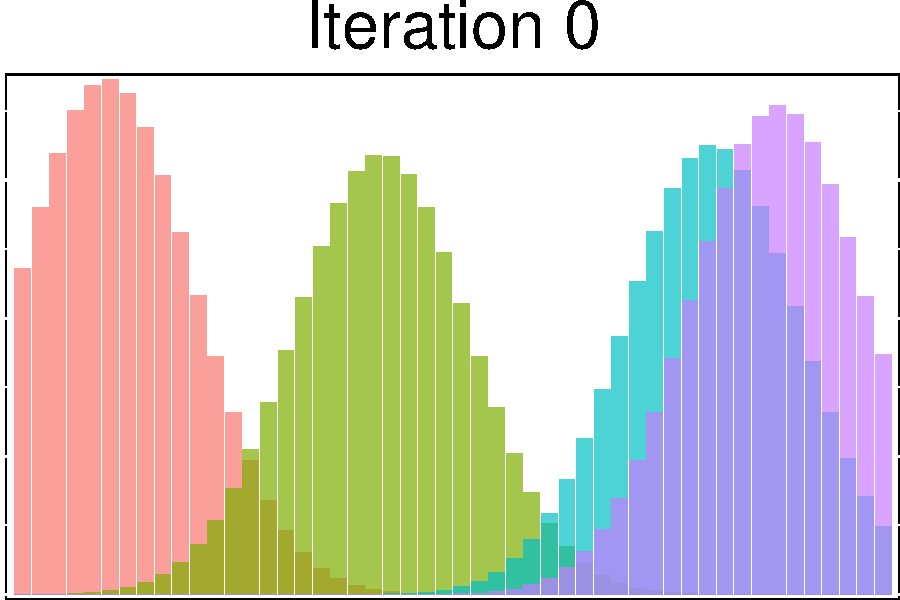
\includegraphics[width=0.19\textwidth]{6_demd/figs/hists/hists_iter_0.pdf}
    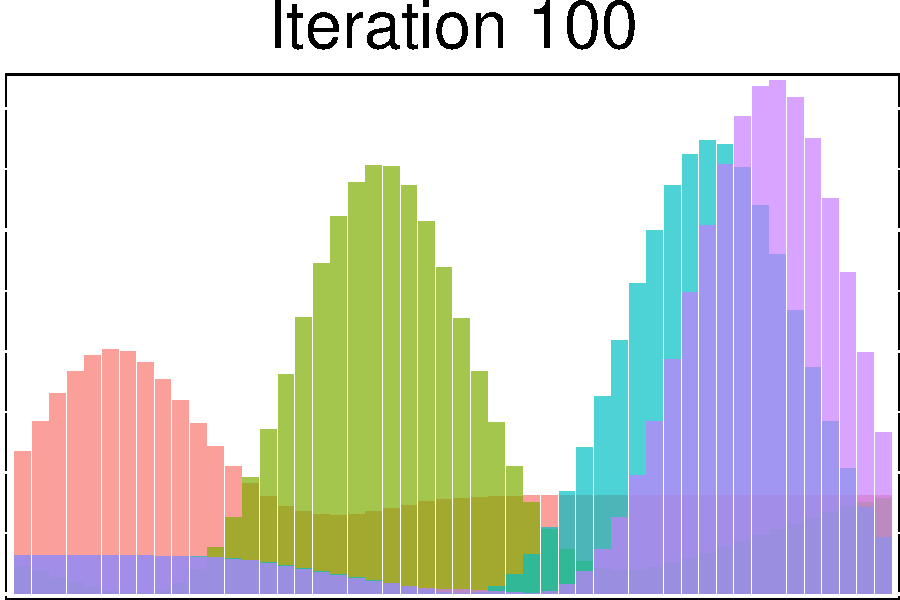
\includegraphics[width=0.19\textwidth]{6_demd/figs/hists/hists_iter_100.pdf}
    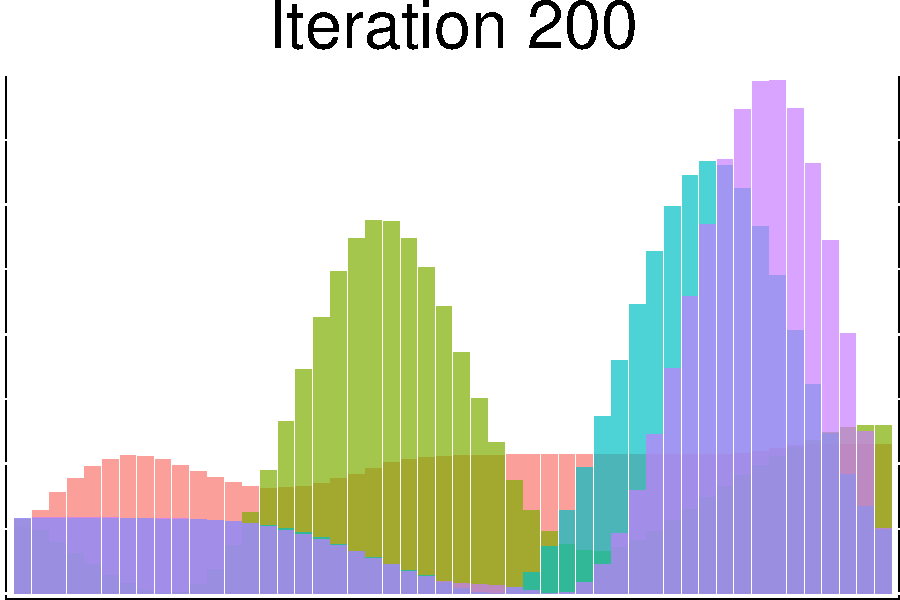
\includegraphics[width=0.19\textwidth]{6_demd/figs/hists/hists_iter_200.pdf}
    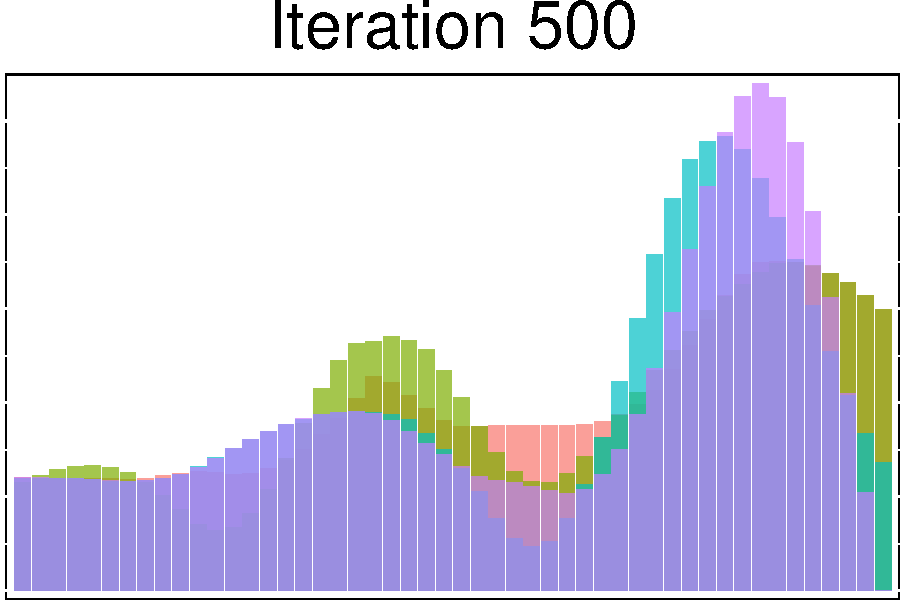
\includegraphics[width=0.19\textwidth]{6_demd/figs/hists/hists_iter_500.pdf}
    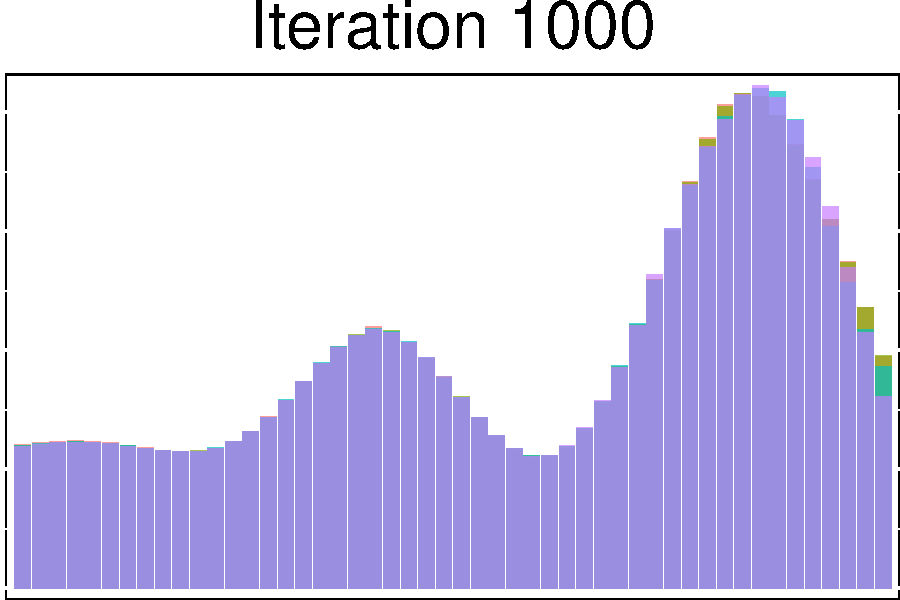
\includegraphics[width=0.19\textwidth]{6_demd/figs/hists/hists_iter_1000.pdf}
    \caption{\footnotesize Starting and ending state of minimizing a multi-marginal OT distance. Each iteration minimizes the generalized Earth Mover's objective, and then updates each histogram in the direction provided by the gradient.}
    \label{fig:hists}
    \vspace{-10pt}
\end{figure}

%%%% OLD
% In this work, we identify a simple {\em global} distributional measure with scaffolding that allows for fast computation over any continuous model output. A new multi-dimensional generalization of the classical Earth Mover's distance has recently been shown to be efficiently computable, and further developments show  that its minimization is extremely fast compared to existing barycenter-style methods.
% Functionally, it
% possesses several useful ingredients: (a) it requires no distributional assumptions, (b) it is efficient to compute, (c) its gradient is also efficiently computable. As a result, the functional can be 
% directly used in regimes where gradients are required for optimization (e.g., backpropogation and other gradient descent methods). 
% Finally, the functional is  numerically stable, and has an intuitive interpretation which facilitates interpretative reasoning.  
% In this work, we identify a simple {\em global} distributional measure with scaffolding that allows for fast computation over any continuous model output. A new multi-dimensional generalization of the classical Earth Mover's distance has recently been shown to be efficiently computable, and further developments show  that its minimization is extremely fast compared to existing barycenter-style methods. Functionally, it
% %distributions are computed over the invariant sets, a barycenter is computed as for the measure of invariance, and heuristic methods are employed to reducing the measured invariance in the loop. 
% Although these approaches aim to directly address the heterogeneity in the model output, they require (1) particular algorithms and solvers for relaxing discrete outputs to enable backpropogation and (2) that operating points and thresholds determining the final prediction are fixed. 
% If a method to operate directly on the activations prior to thresholding was feasible...
% Operating directly on the activations has its own hurdles.
% The activations are continuous, and so distributional assumptions must be made if any computation in the learning pipeline is to remain tractable. However a priori these assumptions are explicitly unknown. 
% \vikas{this appears to be tailored to the above paragraph. Ideally, we should start by highlighting a feature that allows moving away from the pairwise iterative scheme of barycenters.}
% In this work, we observe that a \textit{discretization} of continuous layer outputs allows for the computation of a new multi-distributional generalization of the classical Earth Mover's Distance (EMD) that allows for drop-in computation of disparity at the activation-level. 
% A common application of optimal transport incorporates the concept into a machine learning model by appending a suitable regularization term to the model's objective function.  Typically, this regularization term has the effect of making the statistical distribution of subsets of solutions either more uniform or else invariant in some prescribed way.  An illustration of a prototypical process appears in Figure~\ref{fig:hists}.
% In this paper, we apply a multi-distributional generalization of the classical Earth Mover's distance to the task of regularizing network models.
% The generalization that we employ is based on the classical Earth Mover's Distance (EMD), and
% We demonstrate that this functionally 
% possesses several useful ingredients: (a) it requires no distributional assumptions, (b) it is efficient to compute, (c) its gradient is also efficiently computable. As a result, the functional can be 
% directly used in regimes where gradients are required for optimization (e.g., backpropogation and other gradient descent methods). 
% Finally, the functional is  numerically stable, 
% and has an intuitive interpretation which facilitates interpretative reasoning.  
% Empirical demonstrations of the speed and viability of our approach are presented in Section~\ref{sec:results}.
% We take direct advantage of linear programming formulations of the EMD in its generalized form, and show that in fact the gradient can be directly identified as the solution to the dual program. Recent algorithmic developments allow for the primal and dual to be solved concurrently, allowing for a no-cost gradient computation if the forward computation is chosen accordingly.
% Whereas the classical Earth Mover's distance defines a distance metric between pairs of distributions, the generalized Earth Mover's objective defines a natural way to  measure  dissimilarity amongst $d\geq 2$ distributions. 
% Both the classical distance and the generalized objective can be expressed as linear programs.
% One advantage of the linear program formulation is the fact that every linear program has an equivalent {dual} linear program.
% We demonstrate, using standard sensitivity analysis, that solutions to the dual linear program equal the primal objective functional's gradient. If the functional is regularizing a neural network model, this gradient can be used for backpropagation of derivatives during model training.
% Additionally, it was recently shown that solving both the primal and dual linear programs of the generalized Earth Mover's objective can be accomplished in linear time and constant space by applying a straightforward  greedy algorithm. In experiments, we compare the speed to compute the gradients of the generalized Earth Mover's objective of the greedy algorithm against native auto-gradient procedures, and we demonstrate over $1000$-fold speed improvement. The method we describe is numerically stable, as no division operations or unusually large quantities are invoked in the process of solving the linear programs.  
% In many settings, however, a strict set of assumptions is required to apply and compute these existing methods. Particularly, optimal transport measures over continuous spaces are only practical when strong distributional assumptions can be made, and while discrete assumptions allow for more broad computation, they tend to poorly capture and generalize the actual measures of interest.
% An important feature of our approach is that it acts on model outputs prior to thresholding, so invariances to be maintained across varying thresholds.
% Our procedure addresses both of these limitations directly, by first promoting invariance at all discretizations of model outputs \textit{prior to thresholding}, and by making use of a differentiable histogramming procedure to directly apply precomputed gradients through backpropagation.
% A challenge in practical implementations that use this architecture  define invariance can be based on business or regulatory constraints, but these constraints can change over time.  Industry deployments of ML pipelines are not compatible with such a setting is an important way: thresholds considered for discretization or classification are often adjusted or changed due to changing business or regulatory directives.   After training with procedures similar to the above, no guarantee regarding invariance can be made if the threshold is changed. It is often not sufficient or even feasible to retrain when operating points may or must change.
% {\color{red} redundant, merge with above para}
% \noindent\textbf{Contributions.} In this work, we present an application of a recent extension of the classical Earth Movers distance to a higher-dimensional Earth Mover's objective.
% We show that minimization of the objective leads to the harmonizing (lang) of input distributions similar to the minimization of distributions to barycenters.
% We prove theoretical properties of the objective and the procedure that
% reveals the gradient can be read directly off from a primal/dual algorithm,
% alleviating the need for computing intensive pairwise couplings.
% % This objective provides an alternative to barycenter approaches as a way to regularize network models in a way that reduces statistical dissimilarity of the optimal solutions. % The functional we use acts on a \textit{discretized version} of model outputs prior to thresholding, and allows for invariances to be maintained across varying thresholds. 
% With a particular instantiation of differentiable histograms, we can apply and smoothly operate directly on network activations to compute the EMD measure. 
% We establish through experiment that the speed of computing gradients used in backpropogation can be computed in substantially shorter times than one can achieve using standard tools, due to rapid access to solutions of the the dual linear program formulation.
% We compare and contrast the performance and speed of our construction against Barycenter-like measures in a number of settings and demonstrate applications in a common fairness setting.
% Our final construction integrates seamlessly with existing neural network pipelines.
% Machine learning has become ubiquitous, but has suffered some setbacks in public and regulatory visions due to issues typically considered orthogonal to traditional measures of success within the literature.
% Most modern advancements in machine learning follow from learning a model that optimizes for some measure of \textit{accuracy}, measured by misclassification errors over all samples or global measures of true and false positive and negative rates.
% Unfortunately, when statistical assumptions of homogeneous data fail, these measures can be skewed heavily towards subsets of the data that follow a majority or the primary mode of the underlying distribution. These biases can take many forms, and in applications in which data and outcomes may be represent people and decisions for those people, can lead directly towards unfairness and disparity among groups.
% The last few years of machine learning deployment has revealed a myriad of situations in which strong bias and fairness concerns have led to strong social backlash. Examples: COMPAS, twitter, etc. \cite{?}
% With these concerns has also come interest in technical solutions to fairness and bias. Several conferences and workshops have been created \cite{fat, facct, etc}, devoted to grounding and understanding these ideas within a mathematical and statistical context. From these communities concrete definitions have been formed, along with a number of algorithmic solutions to both avoid and account for bias and unfairness within both data and models.
% Existing methods for accounting for fairness typically define measures over discrete output spaces, and attempt to minimize some measure of disparity between these discrete probabilities. Varying definitions of fairness have been constructed under this umbrella, and a number of nice solutions have been proposed that allow for fair regularization in traditional machine learning training pipelines.
% A drawback to these approaches is that they rely on the discrete/binary outputs of models to be fixed: once a model is trained, the threshold used for those outputs cannot be changed else all fairness guarantees provided by the regularization fail, because the output distributions have all been constructed with that specific threshold. Practical deployments of machine learning models in industry rely on being able to select different points of operation, to match secondary requirements or measures provided by business or regulatory requirements. In these cases it is not sufficient or feasible, especially for large models, to create and retrain methods when these operating points must change. Their is a clear need for methods which are fair across potentially many points of operation.
% While moving to fairness over the continuous measure prior to thresholding may be infeasible, new results suggest that discretization at points of operation can lead to practical solutions for constructing models fair over many thresholds.
% \noindent\textbf{Contributions.} In this work, we analyze fairness from a new perspective. By looking at the distances between distributions over discretized spaces prior to thresholding for downstream discrete tasks, we apply a recently developed tool for computing EMD distance to quickly measure the disparity between groups over discretized continuous measures. Using a key observation that the gradients are readily available, we directly incorporate this EMD distance into standard machine learning pipelines. 
\section{Related Work}
%While machine unlearning has been studied by many in the field, to the best of our knowledge we are the first to propose 
To contextualize our contributions, 
we briefly review existing proposals for machine unlearning. 

\noindent\textbf{Na\"ive, Exact Unlearning.}
A number of authors have proposed methods for exact unlearning, in the case where $(\epsilon=0, \delta=0)$. SVMs by \cite{romero2007incremental,karasuyama2009multiple}, Na\"ive Bayes Classifiers by \cite{cao2015towards}, and $k$-means methods by \cite{ginart2019making} have all been studied. 
%More recently, \cite{} develop methods for Random Forests.
But these algorithms do not translate to stochastic models with millions of parameters.

\noindent\textbf{Approximate Unlearning.} 
With links to fields such as robustness and privacy, we see more developments in approximate unlearning under Definition~\ref{def:forget}. 
The so-called $\epsilon$-certified removal by \cite{guo2019certified} puts forth similar procedures when $\delta=0$, and the model has been trained in a specific manner.
\cite{guo2019certified,izzo2020approximate} provide updates to linear models and the last layers of networks, and 
\cite{golatkar2020forgetting,golatkar2020eternal} provide updates based on linearizations that work over the full network, and follow-up work by \cite{Golatkar_2021_CVPR} presents a scheme to unlearn under an assumption that some samples will not need to be removed.

Other recent work has taken alternative views of unlearning, which do not require/operate under probabilistic frameworks, see \cite{bourtoule2021machine,neel2021descent}. These schemes present good guarantees in the absolute privacy setting, but they require more changes to  pipelines (sharding/aggregating weaker models) and scale unsatisfactorily in large deep learning settings.
\section{Background}
% Before stating the generalized Earth Mover's problem, it is helpful to have a complete description of the classical program.  No new concepts are required to understand the general program once the classical program has been grasped. 
% \noindent\textbf{Notations.}

Denote by $[n]\coloneqq\left\{1,\ldots,n\right\}$, the set of positive integers no larger than $n$. For elements $x\in\RR^{n}$, we denote the $i$th entry of $x$ as $x(i)$, e.g.,  
for any $x\in\RR^{n}$, $x=(x(i):i\in[n])$.    
The positive orthant of $\RR^n$ is denoted $\RR_{+}^{n} \coloneqq \left\{x\in\RR^{n}:x(i)\geq 0, i\in [n]\right\}$. 
We denote by $e\coloneqq (1,\ldots,1)\in\RR^{n}$ the constant vector. 
For $q\geq 1$, we define the $q$-norm  as $\norm{x}_q\coloneqq \left(\sum_{i\in[n]}\left|{x(i)}\right|^{q}\right)^{1/q}$, and if $q$ is suppressed, then $\left\|x\right\|\coloneqq \left\|x\right\|_2$. 
A discrete probability distribution is a point $p\in\RR^{n}_+$ with $e'p=\norm{p}_1=1$.

Given a pair of discrete probability distributions $p_1,p_2\in\RR^{n}_+$, we may want to quantify similarity or dissimilarity. 
%$p_1$ and $p_2$ are. 
Often we do this by selecting from many measures, including the $q$-norm, KL-divergence or the Earth Mover's Distance (EMD).
%
% \vikas{describe that we want to find how similar $p_1$ and $p_2$ are}
%This problem is most well known as discrete optimal transport, or the Earth Mover's problem, and can be described as a linear program.
The EMD for a pair of distributions has several equivalent interpretations. First, let $p_1$ be a source of mass, and $p_2$ be a sink for mass, and  $x(i,j)$, where  $x\in\RR^{n\times n}$, represent the flow of mass from $p_1(i)$ to $p_2(j)$.
Denote by $c(i,j)$ the cost of moving one unit of mass from  $p_1(i)$ to $p_2(j)$.
The EMD between $p_1$ and $p_2$ is the minimal cost to transform $p_1$ into $p_2$, 
%given by the sum of the costs associated with shifting mass, according to $x(i,j)$ such that $p_1$ is transformed into $p_2$.
% Unless otherwise specified, we assume $c(i,j)=|i-j|$, which corresponds to ground distance. 
%This can be 
written as a linear program (LP):
\begin{align}\label{eq:2demd}
\begin{aligned}
\underset{{x\in \RR^{n\times n}_+}}{\textrm{min}} \sum_{i,j} c(i,j) x(i,j) \quad  \textrm{s.t.}\quad \sum_j x(i,j) &= p_1(i); \ 
\sum_i x(i,j) = p_2(j),\ (\forall i,j\in[n]).
\end{aligned}
\end{align}
The source-sink interpretation is asymmetric in $p_1$ and $p_2$, but the LP is symmetric in $p_1$ and $p_2$.  It can be shown that the objective value of this LP defines a {\em metric} \citep{kantorovich1960mathematical}, and the optimal value of the objective function can be interpreted as a distance between $p_1$ and $p_2$,  %For this reason, the Earth Mover's Distance is 
and useful to quantify dissimilarity between pairs of distributions. In particular,  $p_1=p_2$ if and only if the optimal objective value of the Earth Mover's problem vanishes.
%
%Since the Earth Mover's program is a linear program, it has 
The LP in (\ref{eq:2demd}) has an equivalent dual LP, 
%which has the form
\begin{align}\label{eq:2dualemd}\begin{aligned}
    &\underset{z_1,z_2\in\RR^{n}}{\textrm{max}} z_1'p_1 + z_2'p_2 \quad 
    \textrm{s.t.}\quad  z_1(i) + z_2(j)\leq c(i,j),\  (\forall i,j\in [n]).
    \end{aligned}
\end{align}
By strong duality, the optimal value of the primal program~(\ref{eq:2demd}) equals the optimal value of the dual program (\ref{eq:2dualemd}). 
% We show below that a solution to dual program is useful for computing gradients.
Many practical relaxations have been proposed for (\ref{eq:2demd}), including entropic regularization \citep{cuturi2013sinkhorn}.
%, which is notable for being both practical and scalable.
%as it has led to practical approximations over large histograms.
Computation of the EMD is readily available as in the Python Optimal Transport (POT) library \citep{flamary2021pot}.

%Minimization of the EMD is feasible via backend-supported implementations such as POT \citep{flamary2021pot}.


% This can equivalently been seen as identification of a joint distribution $x$ with both $p_1$ and $p_2$ as marginals, where the total energy of the joint $x$ is minimized under some cost $c$. 
% Other interpretations include the flow of mass between a source and a sink.




% Outcome variable $Y$, discrete random. $y \in \{0,1\}$.
% Sensitive Attribute $A$, random discrete variable. $a \in A$.

% A sample may be a tuple of $\{x_i, a_i, y_i\}$, and a model may take in the subset $\{x_i, a_i\}$ and generate a prediction $\hat{y}_i = f_\theta(x_i, a_i)$. Dataset $S:= \{x_i,a_i,y_i\}_{i=1}^n$. A fairness measure $G(a,y,\hat{y})$.

% Demographic Parity
% \begin{align}
%     G(a,y,\hat{y}) &= p(\hat{Y} = \hat{y} | A = a) \\
%     g(S, a, y, \hat{y}) &= \frac{1}{n} \sum_{i=1}^n \II[a_i = a, \hat{y}_i = y] \\
%     &= p_a
% \end{align}
% $Y$ binary, so we don't need to distinguish $p_a$ for different $y$.

% Fairness across all groups $\forall a \in A$ requires finding a point (model, parameters, $\theta$) where these probabilities are close.
% \begin{align}
%     \theta^* = \min_{\theta} \sum_{i,j} d(p_{a_i},p_{a_j})
% \end{align}
% For each group, there may be an optimal $\theta_a$. Then we can rewrite the problem as
% \begin{align}
%     \theta^* = \min_{\theta} \sum_a d(\theta,\theta_a)
% \end{align}
% General formulation \cite{jiang2020wasserstein} requires computing the wasserstein-1 barycenter, computationally intensive, many approximations, complicated algorithm, requires entropic regularization, sinkhorn iterations.

% Many calls to 1-d wasserstein problem.
% \begin{align}
%     d(\theta_1, \theta_2) = &\min \langle P, C \rangle \\
%     &s.t. \sum_j P = \theta_1,\ \sum_i P = \theta_2
% \end{align}
% For fairness with two groups, the distributions can be the conditional fairness definitions (DP, EO, etc.).

% How about with d groups? d-dimensional tensor.
% \begin{align}
%     \min \langle P, C \rangle_{\otimes}
% \end{align}
% How do we solve this efficiently? \cite{kline2019properties}
% Kline 2019: d-dimensional Earth Movers.

% Main technical piece: Using new solutions to the d-dimensional EMD for barycenter computation.

% d-dimensional earthmover's problem.
% \begin{align}\label{eq:dEMD}
%     &\min \sum_{I \in \cI} C_I P_I \\
%     &s.t. \sum_{I\setminus j} P_{I\setminus j} = x_j \quad \forall j \in \{1,\ldots, d\}
% \end{align}

% \subsection{Subgroup Fairness}

% We may not only have one sensitive attribute $A$. Let $\cA$ be a collection of binary attributes. In this case, if we would like to be fair for all groups, simply enforcing the above definitions for each groups would work, but may not necessarily lead to fairness for various \textit{intersections} of subgroups. In this case, what we may be interested in is subgroup fairness. 

% Following traditional definitions, let $G \in \cG$ be a specific subgroup for which we wish to be fair to, identified by a binary variable defined as the intersection over the $A$'s for each larger group. For example, we may have $A_1$ as race and $A_2$ as gender, and we may wish to be fair towards an intersection $G := A_1 \cap A_2$.

% This definition also allows for one-hot encodings of categorical variables, and intersections of different categorical variables.

% It is easy to see that with many different groups and subgroups we may wish to be fair to, the total set size of $\cG$ grows exponentially with the number of sensitive attributes. 

% Following a traditional approach of optimizing each group towards a globally fair model is not feasible for existing Wasserstein-style approaches.

% Entropic regularization approaches with Sinkhorn iterations grow with the number of distributions, and computing Wasserstein barycenters for many groups via the above formulations requires computing barycenters over all subgroups and estimation of these centers become worse with more samples. (See below for speed comparisons)

\subsection{Discrete Multi-Marginal Optimal Transport}

%The natural next step from above is an extension when we have an arbitrary number of $d>2$ distributions. 
%A limitation of t
The foregoing approach 
%is that it 
applies only to $d=2$ distributions, namely $p_1$ and $p_2$. We briefly review the extension 
%of the above idea 
to $d>2$ distributions; 
%. The optimal transport 
the literature calls this \textit{multi-marginal optimal transport (MMOT)}.%, with similar subproblems following problem and cost-specific assumptions a la Kantorovich and Monge. Here we focus on the discrete setting.
% \vikas{give the reader a sense of whether this is still background material and/or where this is going.}

\begin{definition}[Discrete Multi-Marginal Optimal Transport (d-MMOT)]\label{def:dmmot}
Let $p_1, \ldots, p_d\in\RR^n_{+}$ be discrete probability distributions. %Then, $e'p_i=1$ for all $i\in[d]$. % with each $p_i \in \Delta^n$, where $\Delta^n$ is the $n$-dimensional simplex. 
%Let $c_d : \cX^d \rightarrow \RR_{\ge 0}$. 
Let $C_d : \RR^{n^{d}}\rightarrow \RR_{+}$. 
The discrete multi-marginal optimal transport problem (d-MMOT) can be written as
\begin{align*}%\label{eq:dmmot}
    %&\underset{{X \in \cX^d}}{\textrm{minimize}}\quad C_d(X) \\
    &\underset{{X \in \RR^{n\times \cdots \times n}}}{\textrm{min}}\quad C_d(X) \quad \textrm{s.t.}\quad X_i = p_i,\ (\forall i\in [d]),
\end{align*}
where $X_i \in \RR^n$ is the $i$-th marginal of  $X \in \RR^{n\times \cdots \times n}=\RR^{n^{d}}$.
\end{definition}
Following the original formulation \citep{kantorovich1942}, we will restrict the cost function $C_d(\cdot)$ to the linear map, $C_d(X) \coloneqq \langle c, X \rangle_{\otimes}$, where $c \in \RR_{+}^{n\times \cdots \times n}$ is nonnegative.
%The sequel will focus on the following form of the d-MMOT problem.
Here, the d-MMOT is the LP,
\begin{align}\label{eq:gemd}\begin{aligned}
    \underset{x\in\RR^{n^{d}}_{+}} {\textrm{min}}
    \sum_{i_1,\ldots,i_d} c(i_1,\ldots, i_d)\, x(i_1,\ldots,i_d) \quad \textrm{s.t.}
    \sum_{i_2,\ldots,i_d} x(i_1,\ldots,i_d) &= p_1(i_i), (\forall i_1\in[n])\\
    % &\sum_{i_1,i_3\ldots,i_d} c(i_1,\ldots, i_d)x(i_1,\ldots,i_d) = p_2(i_2),\ (\forall i_2\in[n])\\
    \qquad\vdots\\
    \sum_{i_1,\ldots,i_{d-1}} x(i_1,\ldots,i_d) &= p_{d}(i_{d}), (\forall i_d\in[n]).
    \end{aligned}
\end{align}
This linear program (LP) is central to the regularization schemes that are discussed below.
\section{Efficient d-MMOT Computation}
The linear d-MMOT problem (\ref{eq:gemd}) suffers from the curse of dimensionality: the LP has $n^d$ variables, and even modest choices of $n$ and $d$ can result in a LP with billions of variables, making standard LP solvers inapplicable.
%Traditional linear programming solvers such as interior point methods have been studied in the two-dimensional context, but the MMOT setting does not allow a direct extension given the exponential dependence on $d$. 
Alternatively, specific algorithms have been proposed  \citep{benamou2015iterative}, and 
relaxations via entropic regularization have become more widespread, with very recent extensions to the d-MMOT setting \citep{tupitsa,mmotcuturi}. 

% Putting aside the computation of the dMMOT objective,
% in practical applications its often the case that moving input distributions closer or further from each other requires minimizing or maximizing the objective. Define an arbitrary distance among distributions as $\phi(p_1, \ldots, p_d)$. If this distance is defined as the objective in \eqref{eq:gemd},
% then minimizing the distance among distributions in this form requires bilevel optimization.
% Of course we can set all distributions to be the same for the problem to minimized,


In practice, the cost $c$ in (\ref{eq:gemd}) typically takes one of two forms. In the case where the distributions $p_1, \ldots, p_d$ are over categorical variables, the cost is typically defined as $c(i_1, \ldots, i_d) = 0$ when $i_1 = \cdots = i_d$ and $1$ otherwise.
However, and importantly, if the distributions $p_i$ are histograms over some ordinal or discretized space, 
the cost typically has a structure 
closer to that of a ``tensorized'' distance, characterized by the {\em Monge} property.
%\ronak{emphasize this, it is key to distinguish our construction, maybe add motivation in intro re this}
\begin{definition}[Monge Property]
A tensor $c$ is Monge if for all valid $i_1, \ldots i_d$ and $j_1, \ldots, j_d$, 
%$1 \leq i_1 \leq j_1 \leq n$, $1 \leq i_2 \leq j_2 \leq n$, $1 \leq i_d \leq j_d \leq n$,
\begin{align}
c(s_1, \ldots, s_d) + c(t_1, \ldots t_d) \leq c(i_1, \ldots i_d) + c(j_1, \ldots, j_d)
\end{align}
where $s_k = \min(i_k, j_k)$ and $t_k = \max(i_k, j_k)$.
\end{definition}
Our focus is on a specific cost, which is known to be Monge: $c(i_1,i_2,\ldots,i_d)\coloneqq \max{\{i_k:k\in[d]\}} - \min{\{i_k:k\in[d]\}}$. When $d=2$, this cost reduces to $c(i_1,i_2)=|i_1-i_2|$, which agrees with the classical EMD cost. This choice of $c$ is called the {\em generalized EMD cost}.


%\ronak{this is not explained below, a sentence here in place suggesting how its used in histograms/etc would  be better}

% While the Monge restriction may seem ``nicer" compared to arbitrary nonnegative costs, it is not yet clear how this can be leveraged for efficient computation. 
% The Monge cost does not in itself provide nicer properties to existing methods for multi-marginal optimal transport,
% the program suffers from the curse of dimensionality.
% If $d$ histograms with $n$ bins are being compared, the decision variable of the program still lies in $\RR^{n^{d}}$, which can be very large even if both $d$ and $n$ are modest (say $n=d=10$). 
% To progress in any direction, it is necessary for us to identify a method for taking advantage of this structure in an efficient manner.

%\vikas{the following needs attention. We should think of how to provide some daylight -- because as written, it seems what a reader may call a ``direct application''.}
\begin{remark}Limiting our attention to this cost is not as restrictive as it may appear. 
Indeed, \cite{BEIN199597} shows that the optimal solution to the LP (\ref{eq:gemd}) is independent of the cost, as long as it is Monge.
Additionally, when $c$ is the generalized EMD cost, \cite{kline2019properties} describes a greedy algorithm that solves both (\ref{eq:gemd}) and its dual (\ref{eq:dualgeneralemd}) in linear time. 
% They present an algorithm (presented in Algorithm~\ref{alg:primaldual})
% and constructs a theoretical and algorithmic framework for solving the discrete MMOT.
% Particularly,
% \ronak{key results from kline19, complexity, short description of results}
%\begin{remark}
It is also shown that the optimal objective value is a continuous nonnegative function of each probability distribution $p_j$ (i.e., small changes in one distribution cause small changes in the objective value). Continuity is critical for numerical stability.  Next, when $c$ is the generalized Earth Mover's array, the optimal objective value vanishes if and only if $p_i=p_j$ for all $i,j\in[n]$. 
%\end{remark}
This {\em separability} property is useful in applications where we wish to iteratively ``step towards'' the barycenter of a set of distributions, {\color{blue}see Fig. \ref{fig:min_demd}}.
%{\color{blue} This typically would happen in an {\em outer} loop when training a deep neural network. }
In order to step towards {\color{blue}(red arrows)} a barycenter, we  require a descent direction.  %This is the next result.
%While we can directly push them all towards an arbitrary point in the simplex (e.g., uniform, barycenter), it would be better if we could naturally move towards a point that is close, in some sense, to the initial distributions.
% is relevant since our goal is to regularize the model in a way that favors equi-distribution of mass across multiple probability densities.
We observe that the following  result gives us  this functionality.
\end{remark}

% We can also write the dual linear program.
% \begin{alignat}{2}\label{eq:dualgeneralemd}\begin{split}
% &\underset{z_j\in\RR^n, j\in[d]}{\textrm{maximize}}\qquad\sum_{j} x_j'z_j\\
% &\textrm{subject to}\qquad z_{1}(i_1)+\cdots+z_{d}(i_{d})\leq c(i_1,\ldots,i_{d}),\end{split}
% \end{alignat}
% where the indices in the constraints include all $i_j\in[n]$, $j\in[d]$.

% The following result will make use of the dual linear program.  Before stating the theorem, we introduce some notations. Given distributions $p_1,p_2,\ldots,p_d\in\RR^{n}$ with $e'p_j=1$ for all $j\in[d]$, denote by $\phi(p_1,\ldots,p_d)$, the optimal objective value of the LP in (\ref{eqn:gemd}). Denote by
% \begin{align*}z^*=(z_1^{*}, z^*_2,\cdots,z^*_{d}),
% \end{align*}
% an optimal solution to the dual program~(\ref{eq:dualgeneralemd}).
\begin{theorem}
The dual linear program of the d-MMOT problem (\ref{eq:gemd}) is
\begin{alignat}{2}\label{eq:dualgeneralemd}
\begin{split}
\underset{z_j\in\RR^n, j\in[d]}{\textrm{maximize}}\qquad\sum_{j} p_j'z_j 
\qquad \textrm{subject to}\qquad z_{1}(i_1)+\cdots+z_{d}(i_{d})\leq c(i_1,\ldots,i_{d}),
\end{split}
\end{alignat}
where the indices in the constraints include all $i_j\in[n]$, $j\in[d]$.
Denote by $\phi(p_1,\ldots,p_d)$, the optimal objective value of the LP in (\ref{eq:gemd}). Let $z^*$ be an optimal solution to the dual program~(\ref{eq:dualgeneralemd}).
Then,
% In the established notation, the following two claims hold. First,
\begin{align*}
\nabla \phi(p_1,\ldots,p_{d}) = z^*, 
%\end{align*}
~~\text{and for any $t\in \RR$,}~~
%\begin{align*}
\phi(p_1,p_2,\ldots,p_{d}) = \sum_{j}p_j'
(z_j^* + t\, \eta),
\end{align*}
where $\eta\coloneqq (z_1^{*}(n)\,e, z^*_1(n)\,e, \cdots, z^*_{d}(n)\,e)$.
\label{thm:dualgrad}
\end{theorem}
\begin{proof}
The main observation invokes perturbation analysis \citep{mangasarian1979nonlinear,ferris1991finite} of LPs to assert that, under mild uniqueness conditions, small changes to a LP's input data does not change its optimal solution. The full proof is in Appendix~\ref{sec:app-proof}.
\end{proof}
\begin{remark} The first part of this result provides what we require: a direction of descent. 
Thus, if we can solve the d-MMOT problem and also find the optimal solution to its dual, 
then we can step (or move) our distributions in the opposite direction of the dual variables
to push them together, see Figure~\ref{fig:min_demd}.
The second claim is somewhat technical, and reconciles particular affine shifts that result in equivalent objective values.
\end{remark}

% The second claim, which is rather technical, requires some motivation/explanation for why it was included. 
% We observed empirically that solutions yielded by either autograd or by numerical approximations differed from the solutions yielded by the greedy algorithm that we employ. 
% But the difference was, in all cases, inconsquential: the dual objective functional, evaluated on both vectors agreed, and in all examples tested, the difference equaled a constant factor times the vector $\eta$ that is stated in the theorem.
{\color{blue} 
\subsection{Optimization of d-MMOT}\label{sec:dual}

{\bf Setup.} 
We can now instantiate d-MMOT as an add-on term in a standard machine learning formulation. Concretely, it can be positioned alongside typical learning losses $L(f(x),y;\theta)$ to encourage minimizing distances among $d$ different distributions $g_i\in G, i \in [d]$, $\text{d-MMOT}(f(x),g;\theta)$, i.e., 
$\min_{\theta} L(f(x),y;\theta) + \text{d-MMOT}(f(x),g;\theta)$. 
Within a deep neural network (DNN) architecture, as in some of our experiments,  
several properties of the d-MMOT module are useful:
our results above naturally provide clean operations for computing both the required objective in the ``forward'' pass and gradients in the ``backward'' pass.
}


\begin{figure*}
    \centering
    %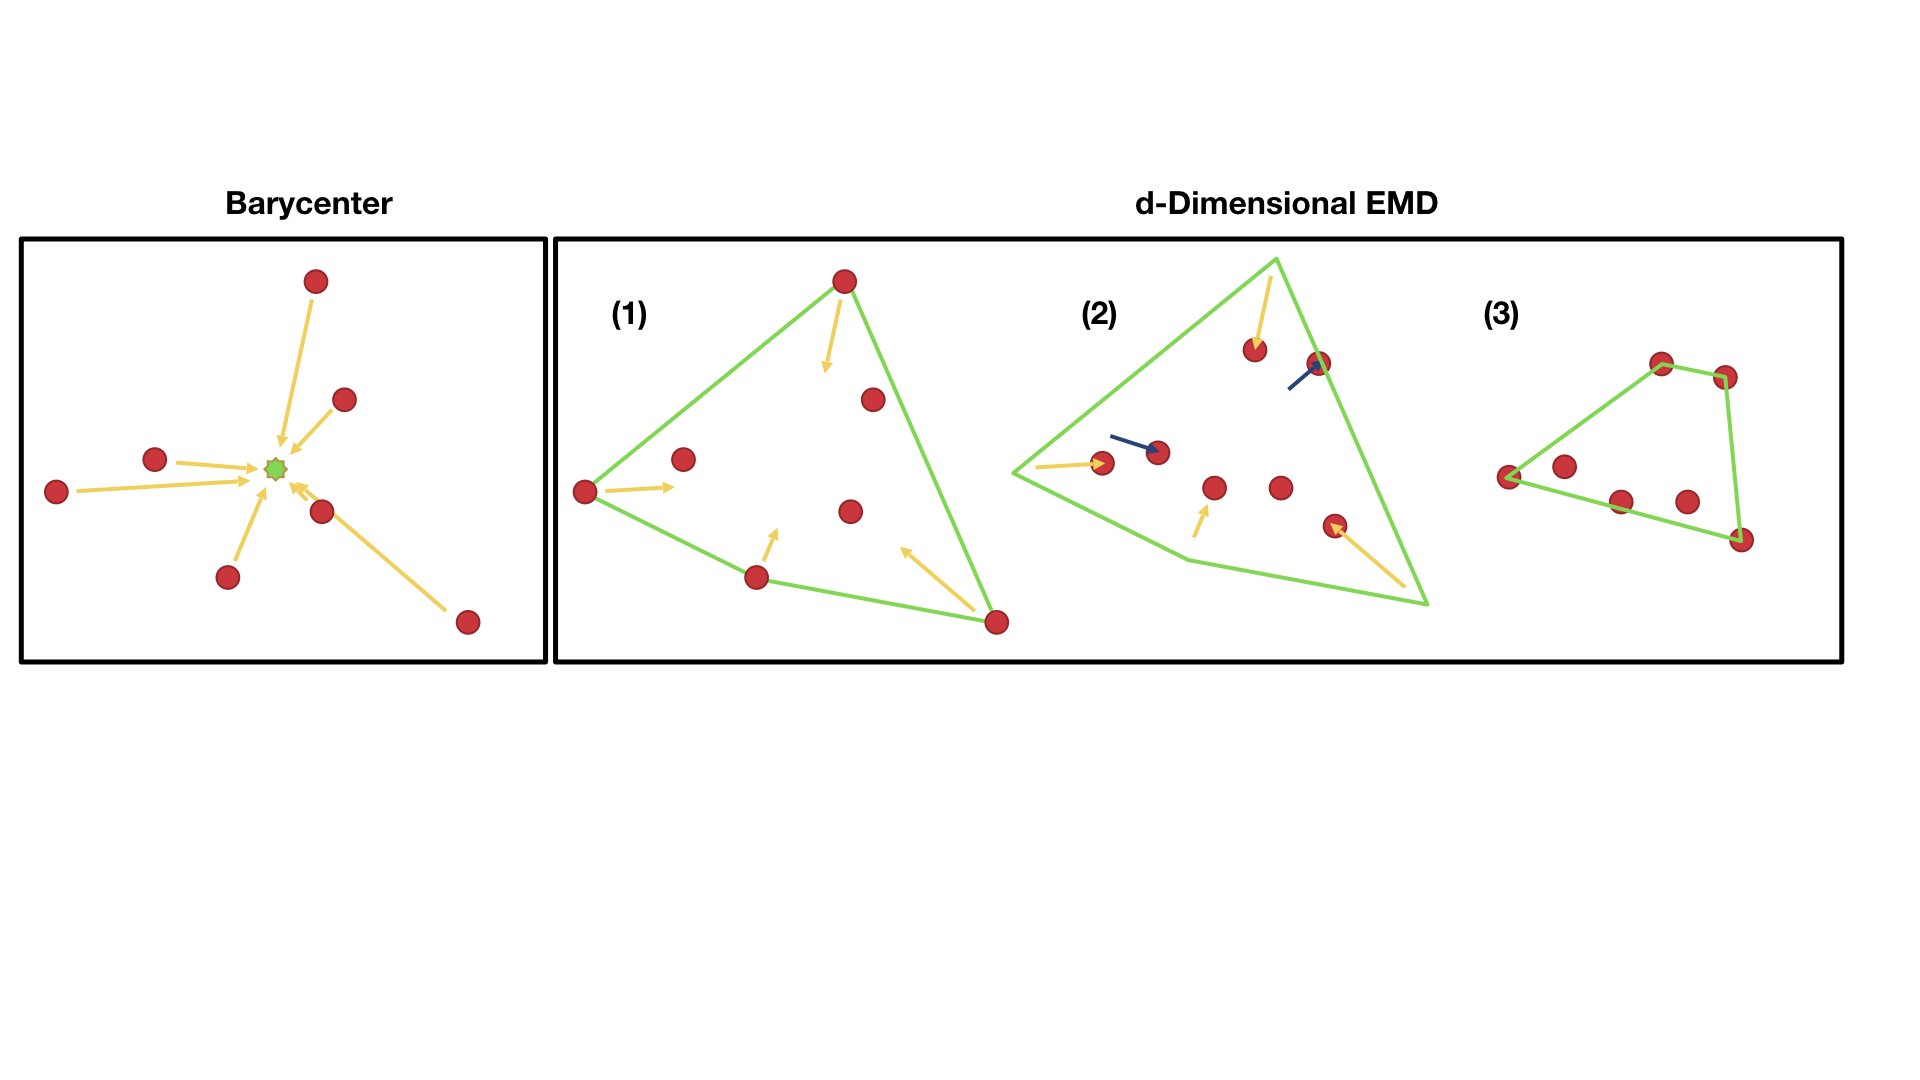
\includegraphics[trim={0 14.5cm 2cm 5cm},clip,width=\textwidth]{6_demd/figs/demd_abstract.png}
    % 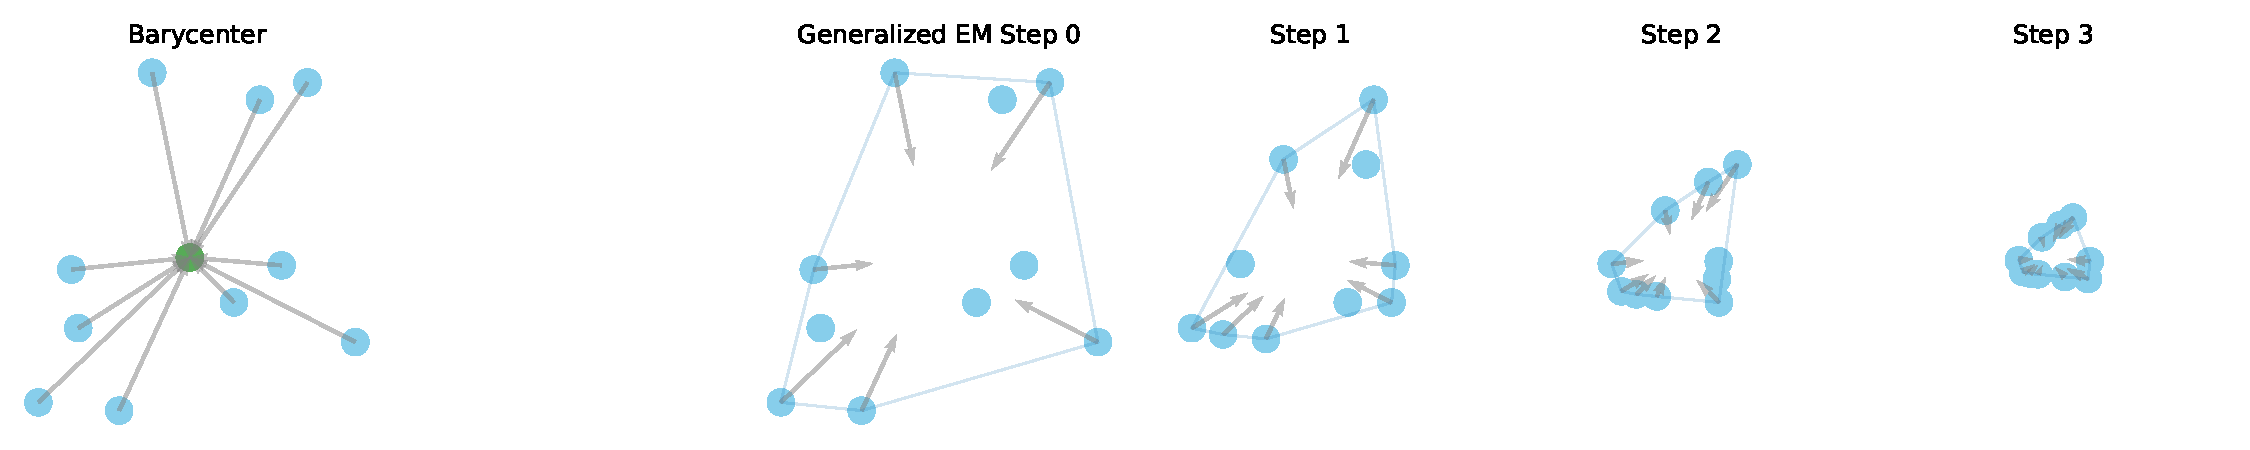
\includegraphics[width=0.95\textwidth]{6_demd/figs/bary-gem-step.pdf}
    %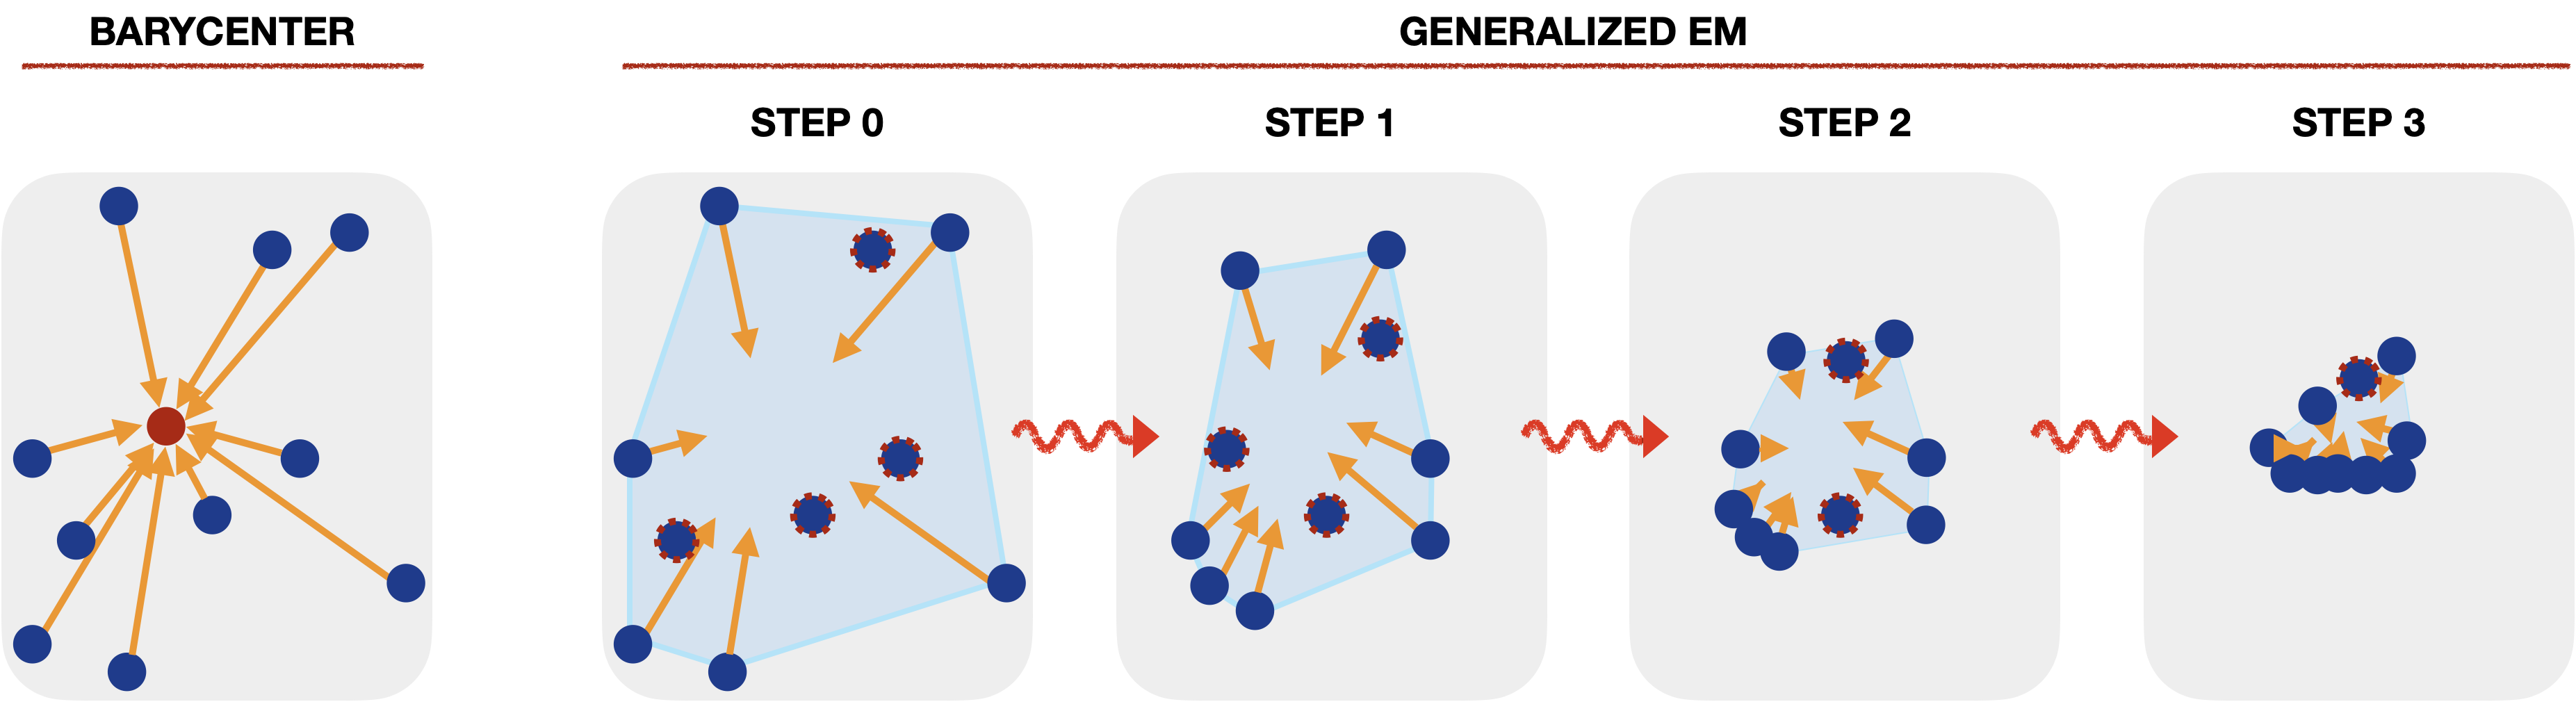
\includegraphics[width=0.9\textwidth]{6_demd/figs/demd_hull_new.png}
    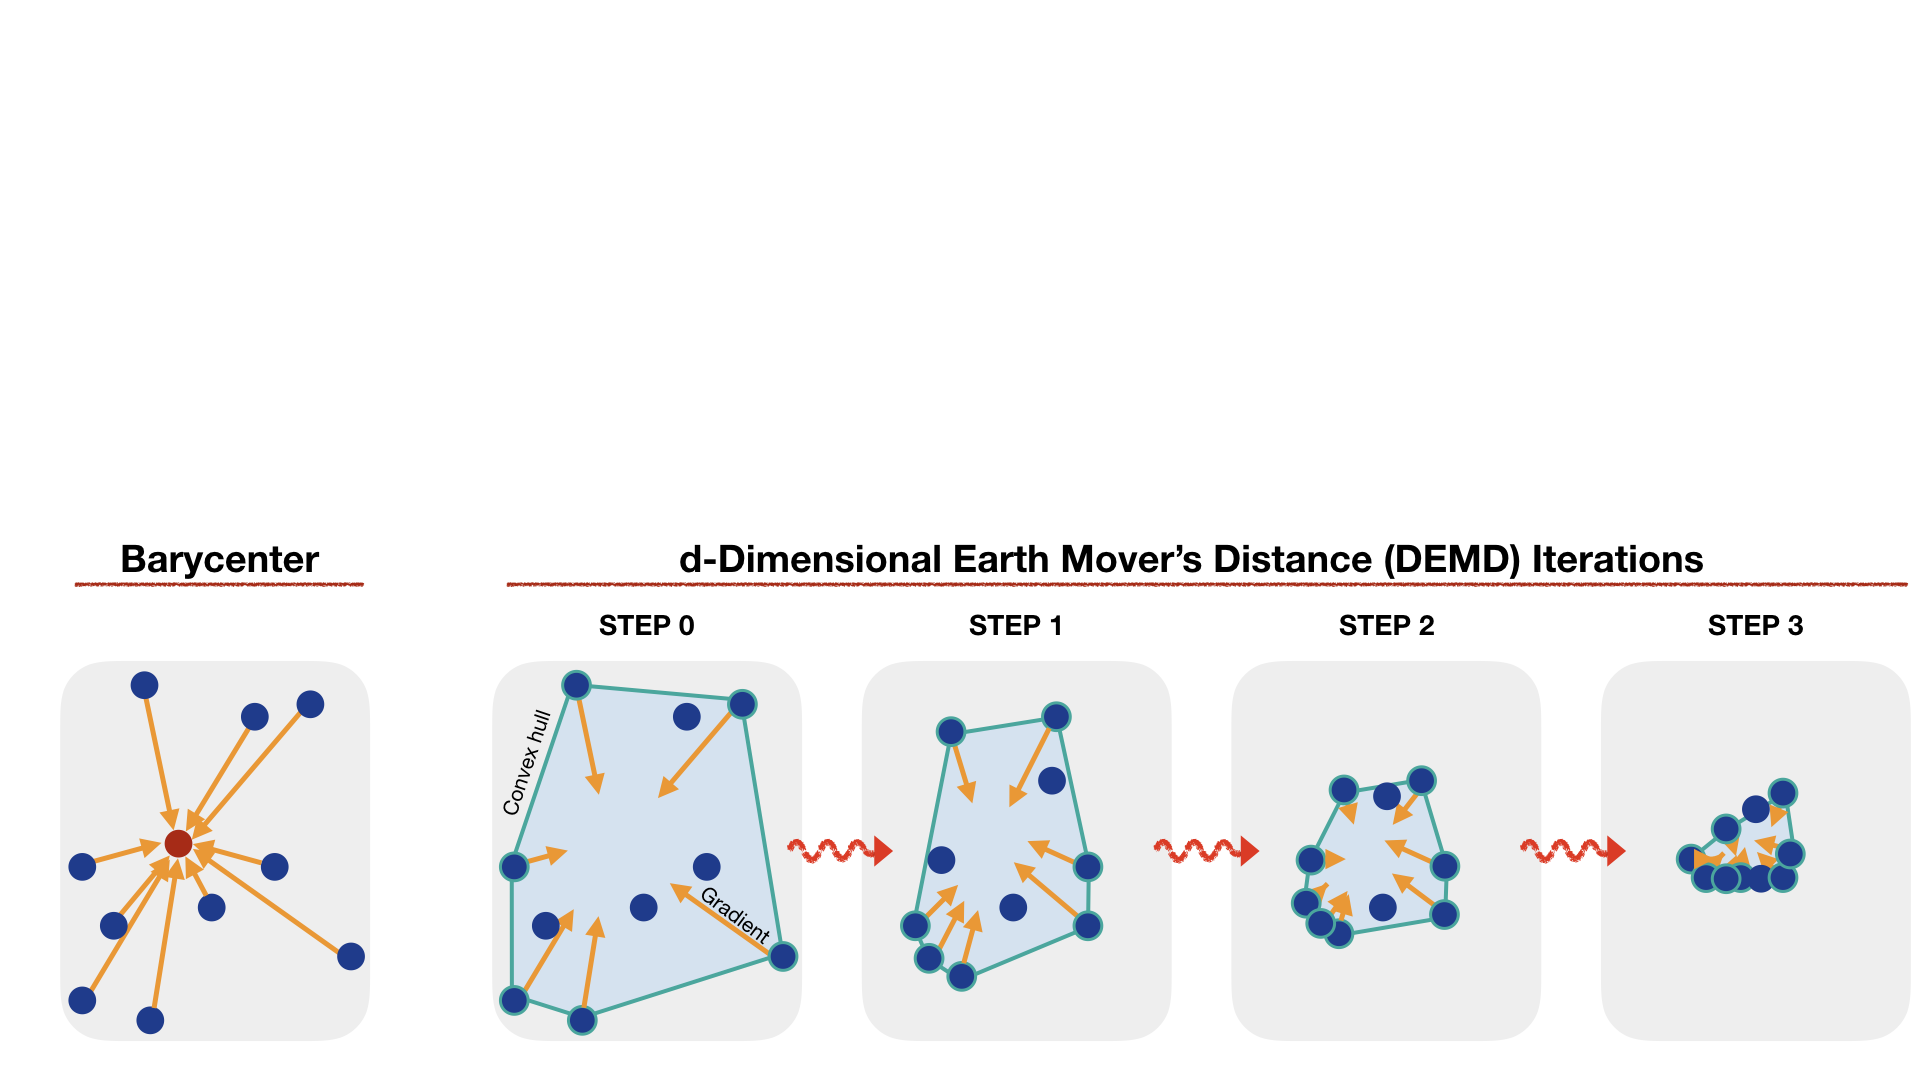
\includegraphics[trim={2cm, 0, 0, 18cm},clip,width=0.9\textwidth]{6_demd/figs/demd_hull_v3.png}
    \caption{\footnotesize ({\em Left}) Barycenter methods identify a center (red circle) and transport \textit{all} distributions (blue circles) toward that center along the coupling path (yellow). ({\em Right}) Our DEMD approach identifies ``support" distributions that lie on the convex hull (outlined circles),  and only those distributions are moved in a direction that decreases the Generalized EMD objective.}
    \label{fig:min_demd}
    \vspace{-5pt}
\end{figure*}

% \subsection{Solving the dMMOT program and its dual}\label{sec:dual}
% JK: this paragraph interrupts the flow
%Using either the iterative Bregman or Sinkhorn-style methods within an outer optimization is  impractical: invoking an interior point solver at each outer iterate explodes an already exponentially large problem, and methods extending two-dimensional entropic relaxations such as unrolling add significant complexity and require approximate solutions.

% Linear program solvers are now a  mature technology,  with polynomial-time guarantees for solution accuracy.
% Despite this, they are unsuitable as the engine that solves the programs of our intended use-case, namely regularizing a network model. 
% Our intent is to have the ability to embed a process that solves an instance of (\ref{eqn:gemd}) and its dual repeatedly during network training.  One reason standard methods are too slow for this is that the programs themselves can be quite large: recall that the cost functional is a dense, rank-$d$ tensor. We note 
% however that there is recent progress towards differentiable LP modules  \cite{meng2020differentiable,NEURIPS2020_6bb56208}. 


% \begin{remark}
% % While recent progress has been made towards differentiable LP modules \citep{meng2020differentiable,NEURIPS2020_6bb56208},
% % here we instead observe that 
% Indeed, these approaches are a necessary path forward given the problem as written,
% where infeasibility is proven for the unregularized formulation (Theorem 3.3 in \cite{mmotcuturi}).
% Notably, their proof follows directly by identifying a form of the cost tensor $C$ such that a reduction to a matching problem leads to a contradiction in theoretical hardness.
% % \vikas{some form of the following sentence needs to be positioned a bit earlier and perhaps repeated here. We need to contrast it with the literature. Is this novel/new etc.}
% In what follows we identify a specific form of the cost tensor $C$ that not only allow for a tractable algorithm, but also has key properties that can be exploited in downstream applications.
% \end{remark}


% In practice, the form of the cost $C$ typically takes two forms. In the case where the distributions $p_1, \ldots, p_d$ are over categorical variables, the cost is typically defined as $c(i_1, \ldots, i_d) = 0$ when $i_1 = \cdots = i_d$ and $1$ otherwise.
% On the other hand, if the distributions $p_i$ are histograms over some ordinal or discretized space, 
% the cost typically follows a structure 
% closer to that of a metric.
% Cost tensors that form these sorts of metrics can be characterized by a tensor form of a distance. \ronak{emphasize this, it is key to distinguish our construction, maybe add motivation in intro re this}
% \begin{definition}[Monge Array]
% A tensor $C$ is Monge if for all valid $i_1, \ldots i_d$ and $j_1, \ldots, j_d$, 
% %$1 \leq i_1 \leq j_1 \leq n$, $1 \leq i_2 \leq j_2 \leq n$, $1 \leq i_d \leq j_d \leq n$,
% \begin{align}
% c(s_1, \ldots, s_d) + c(t_1, \ldots t_d) \leq c(i_1, \ldots i_d) + c(j_1, \ldots, j_d)
% \end{align}
% where $s_k = \min(i_k, j_k)$ and $t_k = \max(i_k, j_k)$.
% \end{definition}

% While the Monge restriction may seem ``nicer" compared to arbitrary nonnegative costs, it is not yet clear how this can be leveraged for efficient computation. 
% The Monge cost does not in itself provide nicer properties to existing methods for multi-marginal optimal transport,
% the program suffers from the curse of dimensionality.
% If $d$ histograms with $n$ bins are being compared, the decision variable of the program still lies in $\RR^{n^{d}}$, which can be very large even if both $d$ and $n$ are modest (say $n=d=10$). 
% To progress in any direction, it is necessary for us to identify a method for taking advantage of this structure in an efficient manner.

% \vikas{the following needs attention. We should think of how to provide some daylight -- because as written, it seems what a reader may call a ``direct application''.}
% Recent work by
% \cite{kline2019properties} leverages the properties of the dMMOT problem with this cost, albeit with a focus on the specific $d$-dimensional earth mover's construction. Interestingly, the algorithm and analysis therein can be leveraged to solve the d-MMOT problem.
% They present an algorithm (presented in Algorithm~\ref{alg:primaldual})
% and constructs a theoretical and algorithmic framework for solving the discrete MMOT.
% Particularly,
% \ronak{key results from kline19, complexity, short description of results}

{\bf Using the primal and dual variables.}  If the optimal objective value of (\ref{eq:gemd}) serves in regularizing a deep neural network, then we can train the network as follows. %this means can compute the objective value during a the forward pass
%The first issue is trivial to implement within standard neural network frameworks. 
% During the forward pass, one can compute the EMD term using the primal/dual greedy algorithm of \cite{kline2019properties}, with one simple modification:  prior to returning, the dual solution variables are stored for use during the backward pass. 
During the forward pass, i.e., computing the d-MMOT objective, we can employ a version of the aforementioned primal/dual algorithm that solely computes the function $\phi$ and stores the dual variables $z$.
As backpropagation proceeds, when the EMD module encounters an incoming gradient, it is simply multiplied by the stored dual variables (see Theorem~\ref{thm:dualgrad} and Algorithm~\ref{alg:demdFunc}). We call our procedure the $d-$dimensional Earth Mover's Distance, or in short,\textit{ the DEMD algorithm}. 

\iffalse
\begin{algorithm}
\caption{Our proposed method: $d-$Dimensional Earch Mover's Distance (DEMD)}\label{alg:demdFunc}
\begin{algorithmic}
 \Function {Forward}{$p_1, \ldots, p_j$}
    \State Compute $\sum s_k t_k$ and $(z_1,\ldots,z_d)$ via the primal/dual algorithm in \cite{kline2019properties}.% \ref{alg:primaldual}.
    \State save $(z_1,\ldots, z_d)$.
    \State \Return $\sum_k s_k t_k$
 \EndFunction
 \Function {Backward}{$\text{gradOutput}$}
 	\State load $(z_1,\ldots, z_d)$
 	\State \Return $(z_1,\ldots, z_d)\cdot \text{gradOutput}$
 \EndFunction
\end{algorithmic}
\end{algorithm}
\fi
\begin{algorithm}
	\caption{ \label{alg:demdFunc} $d-$Dimensional Earch Mover's Distance (DEMD)}
	\SetAlgoLined
	\DontPrintSemicolon
	\SetKwFunction{FVar}{Forward}
	\SetKwProg{Fn}{Function}{:}{}
	\Fn{\FVar{$p_1, \ldots, p_j$}}{
		Compute $\sum s_k t_k$ and $(z_1,\ldots,z_d)$ via \cite{kline2019properties}. \\
		Save $(z_1,\ldots, z_d)$. \\
		\KwRet{$\sum_k s_k t_k$}
	}
	\SetKwFunction{FCore}{Backward}
	\SetKwProg{Gn}{Function}{:}{}
	\Gn{\FCore{$\text{gradOutput}$}}{
		Load $(z_1,\ldots, z_d)$ \\
		\KwRet{$(z_1,\ldots, z_d)\cdot \text{gradOutput}$}
	}
\end{algorithm}


{\bf Complexity.} Computing the DEMD distance in the forward pass is exactly $O(nd)$: linear in the number of distributions and number of bins. This property follows directly from the algorithm, needing only a single pass through all of the data. \cite{BEIN199597} provides this result for greedy algorithms that solve OT programs as in Def.~\ref{def:dmmot}. {\color{blue}  In contrast to methods that derive gradients via entropic regularization schemes, i.e., relaxations of the optimal transport problem \citep{diffpropsinkwass,difftopkOT,quantnorm}, this approach solves the distance computation exactly in linear time.}
This linear time analysis is not only provided by the theory in prior work, but is also explicit in the number of iterations defining our algorithm (see Appendix~\ref{sec:suppdemd} for more details).
For minimizing the DEMD {\color{blue}(computing the updates, i.e., red arrows in Fig.~\ref{fig:min_demd})}, a convergence analysis would follow from the properties of the optimization scheme chosen. Our tool can be dropped in exactly as any other module in modern learning applications (using the observation that gradients are easily computed, i.e., $O(1)$ time to read stored dual variables). %Convergence analysis would follow from the optimization method chosen (SGD, ADAM, etc.).
%}

% It is this construction that we take advantage of and expand upon. 
% \vikas{pose the issue/question first. Then say that we will start from Kline, which we observe can be part of a solution.}

% In this section, we make precise the generalization of the classical Earth Mover's distance. We also state Theorem~\ref{thm:dualgrad}, which establishes that a solution to the generalized linear program's dual equals the gradient of the optimal objective value of the primal linear program.

% \subsection{Multi Marginal Optimal Transport}

% Given a collection of probability distributions $P_1, \ldots, P_m$ over $\cX$, and the cost function $c_m : \cX^m \rightarrow \RR_{\ge 0}$, the multi-marginal optimal transport problem is to minimize $\EE[c_m(X_1,\ldots, X_m)]$ over all couplings of $P_1, \ldots, P_m$, or $X_i \sim P_i$.

% \begin{definition}
% Let $p_1, \ldots, p_m$ be discrete distributions, with each $p_i \in \Delta^n$, where $\Delta^n$ is the $n$-dimensional simplex. Let $c_m : \cX^m \rightarrow \RR_{\ge 0}$. Then the \textbf{discrete multi-marginal optimal transport problem} is
% \begin{align}
%     &\min_{X \in \cX^m}\quad c_m(X) \\
%     &s.t.\quad X_i = p_i \ \forall i
% \end{align}
% \end{definition}

% \begin{proposition}
% Restrict the cost $c_m$ above to be Monge. Then the \textbf{\textit{discretized} multi-marginal optimal transport} is equivalent to the $m$-dimensional earthmover's distance.
% \end{proposition}

% \begin{proposition}
% The d-MMOT or DEMD problem is efficiently solvable.
% \end{proposition}

% \begin{proposition}
% The algorithm results in gradients readily available...
% \end{proposition}


% Before stating the generalized formulation, several points are worthwhile to note. First, the generalized description contains the classical Earth Mover's distance when pairs of distributions are being compared. Second, the generalized program suffers from the curse of dimensionality. If $d$ histograms with $n$ bins are being compared, the decision variable of the program lies in $\RR^{n^{d}}$, and $n^d$ can be very large even if both $d$ and $n$ are modest (say $n=d=10$). 
% However,  this is not an issue in practice: both primal and dual linear programs can be solved using an extremely efficient greedy algorithm, and the decision variable is extremely sparse.

% The classical EMD in (\ref{eq:2demd}) is limited to quantifying dissimilarity between pairs of probability distributions.   But it is useful for applications to be able to break free from this constraint. We describe a framework that matches the classical EMD when pairs of distributions are  being compared, and the framework extends naturally to quantify dissimilarity amongst many probability distributions. To this end, we generalize the Earth Mover's problem stated in the linear program (\ref{eq:2demd}) as follows.  

% {\color{red}:JK motivation, and slow ramp intro}
% Practically, the barycenter is often not even an object of direct interest and instead a means to identifying some direction in which other distributions may be pushed to become closer. Taking advantage of a new algorithm for $d$-dimensional transport problems, we can address a number of the above limitations directly.

% Consider that instead of identifying the barycenter and the sum of pairwise distances, we extend the 2-dimensional problem directly. 

% Let us look closely at the expanded $d$-dimensional earth mover's problem.
% Let $p_1,\ldots, p_d\in\RR^{n}_+$ satisfy $e'p_j=1$ for all $j\in[d]$. 
% Define a cost over the multi-index $(i_1,\ldots, i_d)\in\ZZ^d$ as
% \begin{align*}%\label{eq:cost}
%     c(i_1,\ldots,i_d) = \max\{i_k\}_{k\in[d]} - \min\{i_k\}_{k\in[d]}.
% \end{align*}
% Then, the cost $c\in\RR^{n\times n\times \cdots\times n}$ is a rank $d$-tensor, and when $d=2$, the cost reduces to $c(i,j)=|i-j|$. 
% The generalized Earth Mover's Distance can be written out as 

% The solution to this program effectively identifies a joint distribution $x$ such that the marginals satisfy all $p_j$, and which minimizes the cost. 
% Although the optimal value of the objective function of this program no longer defines a metric when $d>2$, it still possesses several desirable properties.
%, which we use. 
% When used for regularization of machine 
% learning models, a few properties are 
% important to highlight. 

% \subsection{Minimizing dMMOT}
% \ronak{distinction/importance of minimizing the mmot should be made clear above, (shorten/combine sec 3 and 4, shorten intro/related), a central goal of ours is to push dists together, which is hard with other measures.}


% \begin{remark}
% {\bf (1)} The optimal objective value is a continuous function of each probability distribution $p_j$ (i.e., small changes in one distribution cause small changes in the objective value), and 
% {\bf (2)} The optimal objective value vanishes if and only if $p_i=p_j$ for all $i,j\in[n]$.
% \end{remark}
% The first point is critical for numerical stability in applications. The second point is relevant since our goal is to regularize the model in a way that favors equi-distribution of mass across multiple probability densities.

% We can also write the dual linear program.
% \begin{alignat}{2}\label{eq:dualgeneralemd}\begin{split}
% &\underset{z_j\in\RR^n, j\in[d]}{\textrm{maximize}}\qquad\sum_{j} x_j'z_j\\
% &\textrm{subject to}\qquad z_{1}(i_1)+\cdots+z_{d}(i_{d})\leq c(i_1,\ldots,i_{d}),\end{split}
% \end{alignat}
% where the indices in the constraints include all $i_j\in[n]$, $j\in[d]$.

% The following result will make use of the dual linear program.  Before stating the theorem, we introduce some notations. Given distributions $p_1,p_2,\ldots,p_d\in\RR^{n}$ with $e'p_j=1$ for all $j\in[d]$, denote by $\phi(p_1,\ldots,p_d)$, the optimal objective value of the LP in (\ref{eqn:gemd}). Denote by
% \begin{align*}z^*=(z_1^{*}, z^*_2,\cdots,z^*_{d}),
% \end{align*}
% an optimal solution to the dual program~(\ref{eq:dualgeneralemd}).
% \begin{theorem}
% In the established notation, the following two claims hold. First,
% \begin{align*}
% \nabla \phi(p_1,\ldots,p_{d}) = z^*
% \end{align*}
% and second, for any $t\in \RR$,
% \begin{align*}
% \phi(p_1,p_2,\ldots,p_{d}) = \sum_{j}p_j'
% (z_j^* + t\, \eta),
% \end{align*}
% where $\eta\coloneqq (z_1^{*}(n)\,e, z^*_1(n)\,e, \cdots, z^*_{d}(n)\,e)$.
% \label{thm:dualgrad}
% \end{theorem}
% The proof is presented in Section~\ref{sec:proofthm}.

% The second claim, which is rather technical, requires some motivation/explanation for why it was included. We observed empirically that solutions yielded by either autograd or by numerical approximations differed from the solutions yielded by the greedy algorithm that we employ. But the difference was, in all cases, inconsquential: the dual objective functional, evaluated on both vectors agreed, and in all examples tested, the difference equaled a constant factor times the vector $\eta$ that is stated in the theorem.

{\bf A few practical adjustments.}
% In~\cite{kline2019properties}, several properties of the objective functional~$\phi$ are shown. 
% We utilize several of these properties.
% We already observed that $\phi$ is a continuous functional (also stated in Theorem 2.1 of that work). 
% It is also shown there that $\phi$ is homogeneous of degree 1, in the sense that $\alpha\phi(p_1,\ldots,p_d)=\phi(\alpha p_1,\ldots,\alpha p_d)$ for all $\alpha>0$.
It often happens during training that the optimal solutions may, through updates by stepping in the direction of the gradient, acquire entries that are negative. 
This violates an assumption that entries must be nonnegative. However, Thm.~2.2 in~\cite{kline2019properties} shows that the optimal objective value, $\phi$, possesses a type of translation invariance.  We can leverage this result to ensure that, in the event that a point escapes the nonnegative orthant of $\RR^{n}$,
an appropriately constructed constant vector may be added to the current iterate so that it again lies in the nonnegative orthant, \textit{without changing the objective value}. 
Further, with a
% Further, since we wish to compare probability distributions normalized so that $e'p_j=1$ for all $j$, if at some point during training a step modifies $p_j$ so that $e'p_j\not=1$, we can normalize by the positive scalar, $e'p_j>0$. In practice, since each step is a function of a
relatively small learning rate, by the continuity of $\phi$, normalization is a small perturbation of the original point and can be applied as necessary to enforce that updates result in valid distributions. 

\begin{remark}
Another useful property is that if the convex hull of $(p_1,\ldots,p_d)$ is contained in the convex hull of $(\hat{p}_1,\ldots,\hat{p}_{\hat{d}})$, then $\phi(p_1,\ldots,p_d)\leq \phi(\hat{p}_1,\ldots,\hat{p}_{\hat{d}})$, with strict inequality if containment is strict.
A direct consequence of this property is that points within the interior of the convex hull of the data fed to the optimization model have vanishing gradients.
Practically, this leads to \textbf{sparse} gradients w.r.t. the distributions, and nonzero gradients correspond to points on the hull, i.e., distributions which are maximally different from the rest.
Minimization proceeds by iteratively moving mass such that these maximally different distributions are pushed toward each other.
Fig.~\ref{fig:min_demd} shows the convex hull during minimization of the generalized EMD objective via our DEMD algorithm.
\end{remark}

\iffalse % begin removal of histogram wrapfig
\begin{wrapfigure}[15]{R}{0.45\textwidth}
    \vspace{-60pt}
    \begin{minipage}{0.45\textwidth}\vspace{2.5\baselineskip}
    \begin{algorithm}[H]
        \small
        \caption{Differentiable Histograms}\label{alg:diffhist}
        \begin{algorithmic}
        \Function {Init}{$n$} %{\em \hspace*{\fill} // discretization level}
            \State $r := 1/n$;\  %{\em \hspace*{\fill} // bin size};
             $bounds := [0, r, 2r, \ldots, 1]$ %{\em \hspace*{\fill} // bin boundaries}
        \EndFunction
        \Function {Forward}{$acts$}
            \State $counts = []$; $\mathit{cdfs} = \sigma(acts)$ %{\em \hspace*{\fill} // compute CDFs via Sigmoid}
            
            \For{$b \in bounds$}
                \State $cnt = 0$; $dist = \lvert \mathit{cdfs} - b \rvert$ %{\em \hspace*{\fill} // dist. to boundary}
                \For{$i \in [1,\ldots,n]$}
                    \State $cnt = cnt + \operatorname{ReLU}(r - dist[i])$ %{\em \hspace*{\fill} // soft bucket count}
                \EndFor
                \State $counts[b] = cnt$
            \EndFor
            \State $out = counts/sum(counts)$
            \State \Return $out$
        \EndFunction
        \end{algorithmic}
    \end{algorithm}
    \end{minipage}
    %\vspace{-30pt}
\end{wrapfigure} 
% % DO NOT DELETE THE following BLANK LINE 
% % IT IS REQUIRED TO SOLVE A 2-column issue
% % connected to wrapfigure

% \phantom{.} % DO NOT DELETE -- it is required to solve wrapfigure 2-column bug


\fi % end removal of histogram wrapfig

% \subsection{Solving the generalized EMD program and its dual}
% Linear program solvers are now a  mature technology,  with polynomial-time guarantees for solution accuracy.
% Despite this, they are unsuitable as the engine that solves the programs of our intended use-case, namely regularizing a network model. 
% Our intent is to have the ability to embed a process that solves an instance of (\ref{eqn:gemd}) and its dual repeatedly during network training.  One reason standard methods are too slow for this is that the programs themselves can be quite large: recall that the cost functional is a dense, rank-$d$ tensor. We note 
% however that there is recent progress towards differentiable LP modules  \cite{meng2020differentiable,NEURIPS2020_6bb56208}. 

% With a single pass over all input histograms, both the primal and dual decision variables are computed in a sparse manner. The absence of division or scaling also provides numerical stability.
% This simply means the number of bins in histogram $p_i$ need not match the number of bins in $p_j$.



% \begin{algorithm}[ht!]
% \caption{EMD Primal/Dual Algorithm\jeff{do not need to show greedy algorithm here}}\label{alg:primaldual}
% \begin{algorithmic}
% \State {\bf input} $p_j\in\RR^{n}_+$ with $e'p_j=1$ , $(\forall j\in[d])$
% % \State {\bf initialize}
% \State {\em //iteration index, active indices, Eq.~\eqref{eq:gemd} variable, Eq.~\eqref{eq:dualgeneralemd} variable}
% \State  $k \coloneqq 0\in\ZZ$, $I \coloneqq 0\in\ZZ^{d}$, $x \coloneqq 0\in\RR^{n^{d}}$, $z_j\coloneqq 0\in\RR^{n}$, $(\forall j\in [d])$
% % \State  $I \coloneqq 0\in\ZZ^{d}${\em \hspace*{\fill} // track the active indices}
% % \State  $x \coloneqq 0\in\RR^{n^{d}}${\em \hspace*{\fill}  // variable of (\ref{eq:gemd})}
% % \State  $z_j\coloneqq 0\in\RR^{n}$, $(\forall j\in [d])$ {\em \hspace*{\fill}  // variable of (\ref{eq:dualgeneralemd})}
% \While{$I(j) \leq n$, $(\forall j\in[d])$}
%     \State $s_k\coloneqq \min_{j\in[d]} p_j(I(j))$ {\em\hspace*{\fill}  // the mass to move}
%     \State $x(I)\gets s_k$  {\em \hspace*{\fill} // update the EMD solution}
%     \State $p_j(I(j))\gets p_j(I(j))-s_k$, $(\forall j\in d)${\em\hspace*{\fill} // shrink the data}
%     \State $j^*\gets\arg\min_{j\in[d]} p_j(I(j))$
%     \State  $I(j^*)\gets I(j^*)+1$
%     \State $k\gets k+1$
%     \State $t_k\gets c(I)${\em\hspace*{\fill} // cost of this step}
%     \If{ $I(j^*)\leq n$}
%         \State  $z_{j^*}(I(j^*))\gets t_k-t_{k-1} + z_{j^*}(I(j^*)-1)$ {\em\hspace*{\fill} // update the dual solution}
%     \EndIf
% \EndWhile
% \State \Return $x$, $(z_1,\ldots,z_d)$, and the objective value $\sum_k s_k t_k$.
% \end{algorithmic}
% \end{algorithm}

% Algorithm~\ref{alg:primaldual} describes the greedy algorithm that solves both primal and dual generalized Earth mover's programs. The algorithm accepts $d$ distributions (i.e., histograms) $p_1,\ldots,p_d\in\RR^{n}_+$ with $e'p_j=1$ for all $j\in[d]$. 
% Although the algorithm states that all histograms have the same number of bins, the algorithm can be 
% easily adapted to accept as inputs $p_i\in\RR^{n_i}_+$ with $n_i\not=n_j$. 

% \subsection{Minimizing d-MMOT within a loop}
% With a computable generalized EMD objective in hand,
% we now move towards
% %minimizing the d-MMOT problem
% %in modern neural network pipelines.
% %The objective is a concurrent
% the minimization of the appropriate learning loss $L(f(x),y;\theta)$ alongside distances among different distributions $g_i\in G, i \in [d]$, $\text{d-MMOT}(f(x),g;\theta)$, i.e., 
% $\min_{\theta} L(f(x),y;\theta) + \text{d-MMOT}(f(x),g;\theta) $.
% However, note 
% that outputs $f(x)$ and intermediate activations are \textit{continuous} values (layer shape, batch size).
% So, we must transform activations into normalized histograms (i.e., discrete distributions).
% Only once histograms have been generated for different groups of interest can we apply our algorithm and minimize the distances between groups.}

% want to reg. solution found by NNs to a common distribution over all groups.
% common distribution is found with DEMD
% requires computing it
% 
%
% {\bf Precomputed dual variables.} The first issue is trivial to implement within standard neural network frameworks. The ``forward" pass of the EMD module can be defined using Alg.~\ref{alg:primaldual}, with one minor modification.  Prior to returning, the dual solution variables are stored for use during the backward pass. As backpropagation proceeds, when the EMD module encounters an incoming gradient, it is simply multiplied by the stored dual variables (see Algorithm~\ref{alg:demdFunc}).
% \begin{algorithm}
% \caption{Pseudocode of the generalized EMD objective module.}\label{alg:demdFunc}
% % \begin{algorithmic}
% \SetKwFunction{FF}{forward}
% \SetKwProg{FF}{forward}{:}{}
% \FF{($p_1, \ldots, p_j$)}{
%         Get $\sum s_k t_k$ and $(z_1,\ldots,z_d)$ from Algorithm \ref{alg:primaldual}. \\
%         \text{save} $(z_1,\ldots, z_d)$ \\
%         \KwRet $\sum_k s_k t_k$
%   }
% \SetKwFunction{FB}{backward}
% \SetKwProg{FB}{backward}{:}{}
% \FB{(gradOutput)}{
%     \text{load} $(z_1,\ldots, z_d)$ \\
%         \KwRet $(z_1,\ldots, z_d)*gradOutput$
%   }
% \end{algorithm}
% \begin{wrapfigure}[18]{r}{0pt}%{0.45\textwidth}
%     \begin{minipage}{0.45\textwidth}\vspace{2.5\baselineskip}
%     \begin{algorithm}[H]
%         \small
%         \caption{Differentiable Histograms}\label{alg:diffhist}
%         \begin{algorithmic}
%         \Function {Init}{$n$} %{\em \hspace*{\fill} // discretization level}
%             \State $r := 1/n$ %{\em \hspace*{\fill} // bin size}
%             \State $bounds := [0, r, 2r, \ldots, 1]$ %{\em \hspace*{\fill} // bin boundaries}
%         \EndFunction
%         \Function {Forward}{$acts$}
%             \State $cdfs = \sigma(acts)$ %{\em \hspace*{\fill} // compute CDFs via Sigmoid}
%             \State $counts = []$
%             \For{$b \in bounds$}
%                 \State $dist = \lvert cdfs - b \rvert$ %{\em \hspace*{\fill} // dist. to boundary}
%                 \State $cnt = 0$
%                 \For{$i \in [1,\ldots,n]$}
%                     \State $cnt = cnt + \operatorname{ReLU}(r - dist[i])$ %{\em \hspace*{\fill} // soft bucket count}
%                 \EndFor
%                 \State $counts[b] = cnt$
%             \EndFor
%             \State $out = counts/sum(counts)$
%             \State \Return $out$
%         \EndFunction
%         \end{algorithmic}
%     \end{algorithm}
%     \end{minipage}
%     %\vspace{-30pt}
% \end{wrapfigure} 
% % DO NOT DELETE THE following BLANK LINE 
% % IT IS REQUIRED TO SOLVE A 2-column issue
% % connected to wrapfigure

% \phantom{.} % DO NOT DELETE -- it is required to solve wrapfigure 2-column bug

{\bf Need for Histogramming.} 
{\color{blue} Note that outputs $f(x)$ and intermediate activations are \textit{continuous} values (layer shape by batch size).}
So, we must transform activations into normalized histograms (i.e., discrete distributions).
While libraries such as PyTorch and Tensorflow typically provide histogram functions, they are not differentiable. The discontinuous operation of bin assignment does not allow for an end-to-end pipeline where we can push upstream parameters in the direction of minimizing the EMD objective over histograms.
To address this, we 
use a simple relaxed/differentiable histogramming operation. 
First, all outputs are mapped to $[0,1]$ using a Sigmoid activation. Then, for each bin location, the ``count'' in that bin is determined by a ReLU function applied to the difference between the gap between the activation and the distance to the bin boundary. In other words, if an activation falls in a bin, the count of that bin increases based on the distance to the bin boundary, otherwise the count remains the same.
The full procedure is detailed in Appendix~\ref{sec:supphist}.
The ReLU activations defining bin boundaries allow for gradients to move samples towards neighboring bins as needed.

% \noindent\begin{minipage}{.49\textwidth}
% \begin{algorithm}
% % \caption{Differentiable Histograms}\label{alg:diffhist}
% \begin{algorithmic}[1] \footnotesize
% \Function {Init}{$n$} {\em \hspace*{\fill} // #bins, (discretization)}
%     \State $r := 1/n$ {\em \hspace*{\fill} // bin size}
%     \State $locs := arange(0, 1, r)$ {\em \hspace*{\fill} // bin boundaries}
% \EndFunction
% \Function {Forward}{$acts$}
%     \State $cdfs = \sigma(acts)$ {\em \hspace*{\fill} // compute CDFs}
%     \State $counts = []$
%     \For{loc in locs}
%         \State $dist = \lvert cdfs - loc \rvert$ {\em \hspace*{\fill} // dist. to boundary}
%         \State {\em // soft bucket count}
%         \State $ct = \underset{i\in[nbins]}{\sum} \operatorname{ReLU}(r - dist[i])$ {\em \hspace*{\fill} // soft bucket count}
%         \State $counts.append(ct)$
%     \EndFor
%     \State $out = stack(counts)$
%     \State $out = out/sum(out)$
%     \State \Return $out$
% \EndFunction
% \end{algorithmic}
% \end{algorithm}
% \captionof{algorithm}{test}
% \end{minipage}%
% \begin{minipage}[t]{.49\textwidth}
%   \centering
%   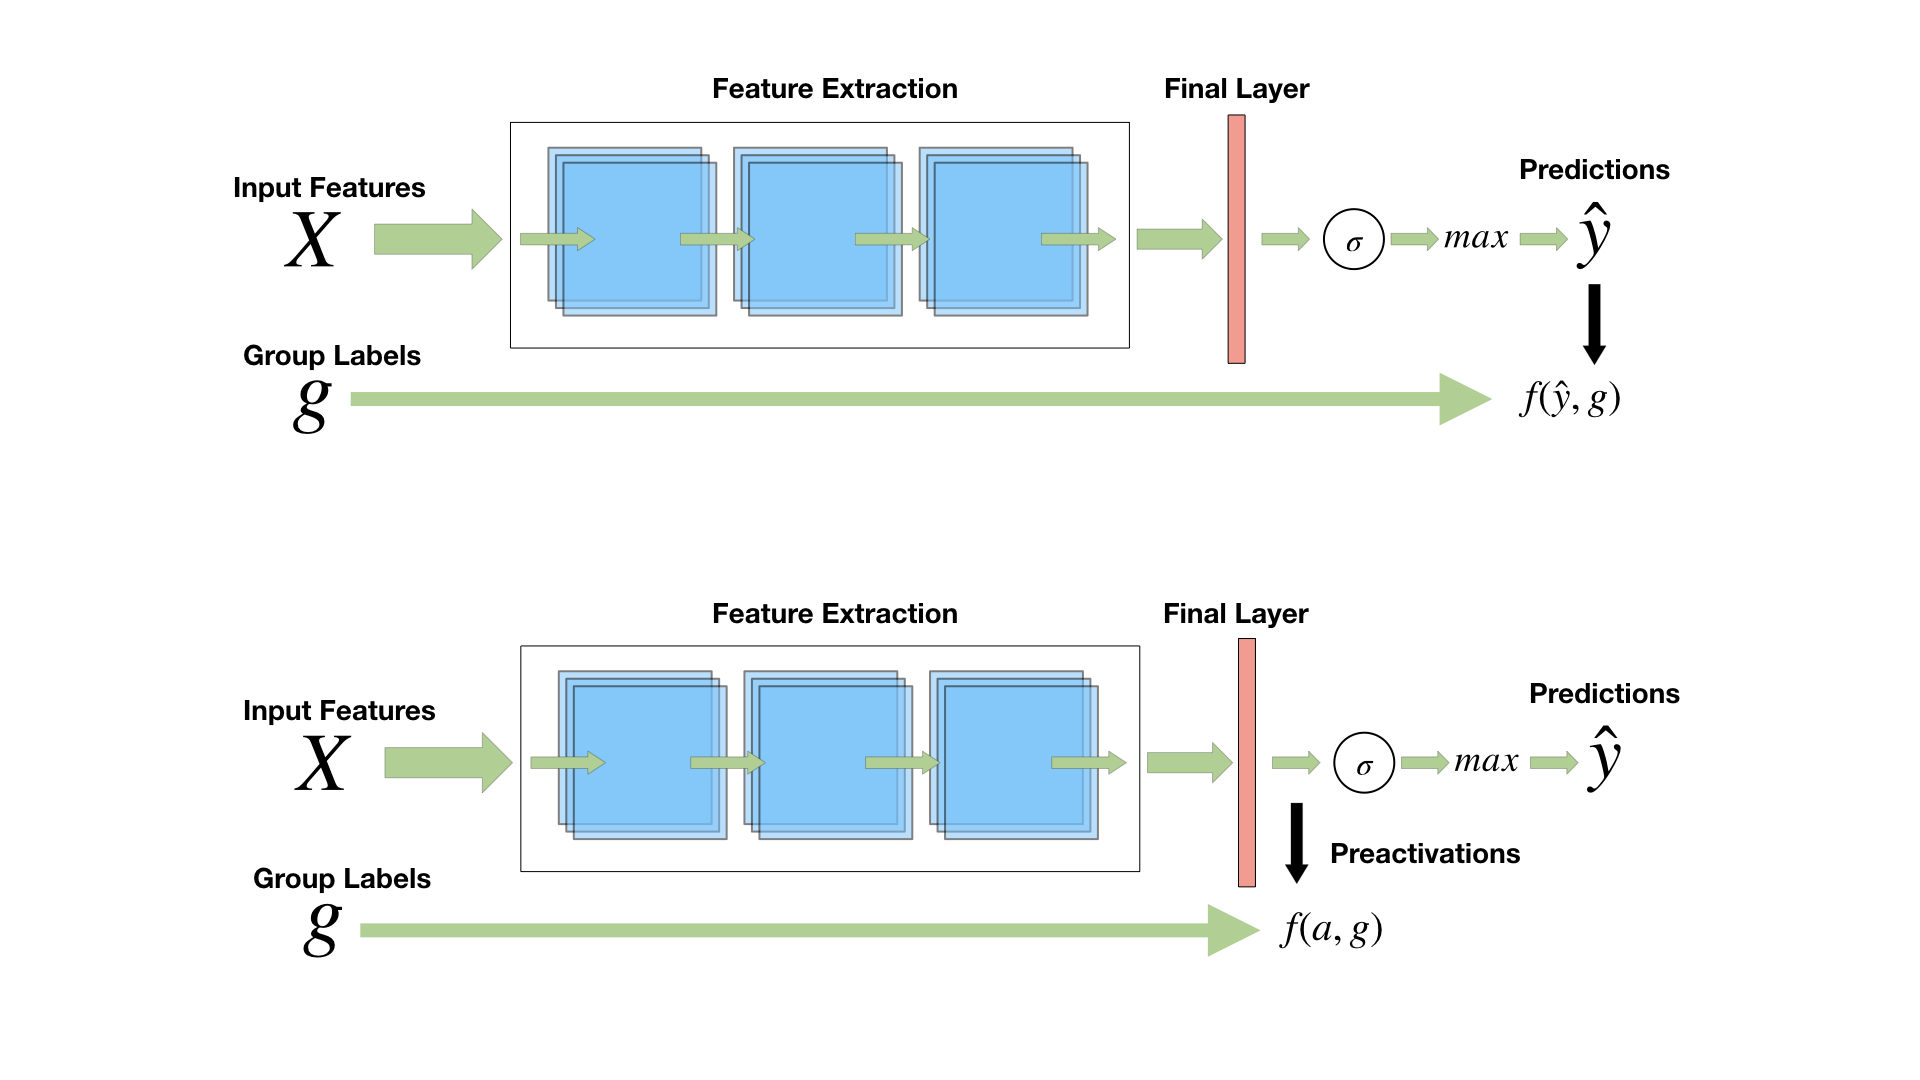
\includegraphics[trim={8cm 0 8cm 0},clip,width=\textwidth]{figs/net_diff.png}
%   \captionof{figure}{This is another figure.} \label{myfig2}
% \end{minipage}



% While gradients are now readily available, typical machine learning pipelines do not have distributions or histograms predefined at outputs which can be fed directly into our EM Loss. Applying existing binning procedures over the batch to estimate histograms will break the ability to autodifferentiate: soft thresholds are necessary at bin boundaries such that samples within a bin may move smoothly as needed. Algorithm \ref{alg:diffhist} provides a differentiable histogram implementation. Using a rectified linear relaxation allows for samples to have a continuous gradient towards neighboring bins.


% \subsection{Minimizing over Multiple Dimensions}
% {\color{red} @Ronak - shall we delete this section?}
%     -extending past simple computation
%     -minimizing DEMD: forcing distributions to become similar wrt to distance
%     -if possible, would lead to another, fast, way to push distributions together/towards "barycenter"

%     minimizing GEM
%     at first does not seem different from existing wass bary approaches
%     requires differentiating through distance computation, updating many times
%     -however particular algorithm of above leads to direct identification of gradients
%     -no backwards derivations/complex derivatives necessary

% \subsection{The dual linear program and back propigation}
% {\color{red}@Ronak - do you want to place backprop comments here or below?}
% The above allows for a direct plug in to existing frameworks. By manually defining the backward pass using the dual variables, the forward pass can be written explicitly and the dual variables stored for backpropagation. 

% \ronak{Will add algorithmic block detailing forward/backward, example in loss/reg formulation}


% Procedure 1:
% \begin{enumerate}
%     \item Given a trained model $\theta$,
%     \item compute the d-EMD distance for all groups
%     \item identify the groups with maximal ``unfairness" via the hull in \eqref{eq:dEMD}.
%     \item Take a coordinate step in reducing the gap.
%     \item Repeat.
% \end{enumerate}


%% This declares a command \Comment
%% The argument will be surrounded by /* ... */
% \SetKwComment{Comment}{/* }{ */}
% \begin{algorithm}
% \caption{Algorithm Pseudocode}\label{alg:main}
% \KwData{$X, Y, G$, algorithm $f$ that learns $\theta$}
% \KwResult{Fair model $\theta$}

% \KwFor{stopping cond} {
%     $\theta_{next} = f(X,Y, G_{prev}, \theta_{prev})$\;
%     Compute EMD for all $G$.\;
%     $G_{next}$ = Select maximally unfair groups via \eqref{eq:floormin}\;
%     $\theta_{prev} = \theta$\;
%     $G_{prev} = G_{next}$\;
% }
% \end{algorithm}
\begin{figure}[t]
\vspace{-0.1in}
    \centering
    \raisebox{\baselineskip}%
    {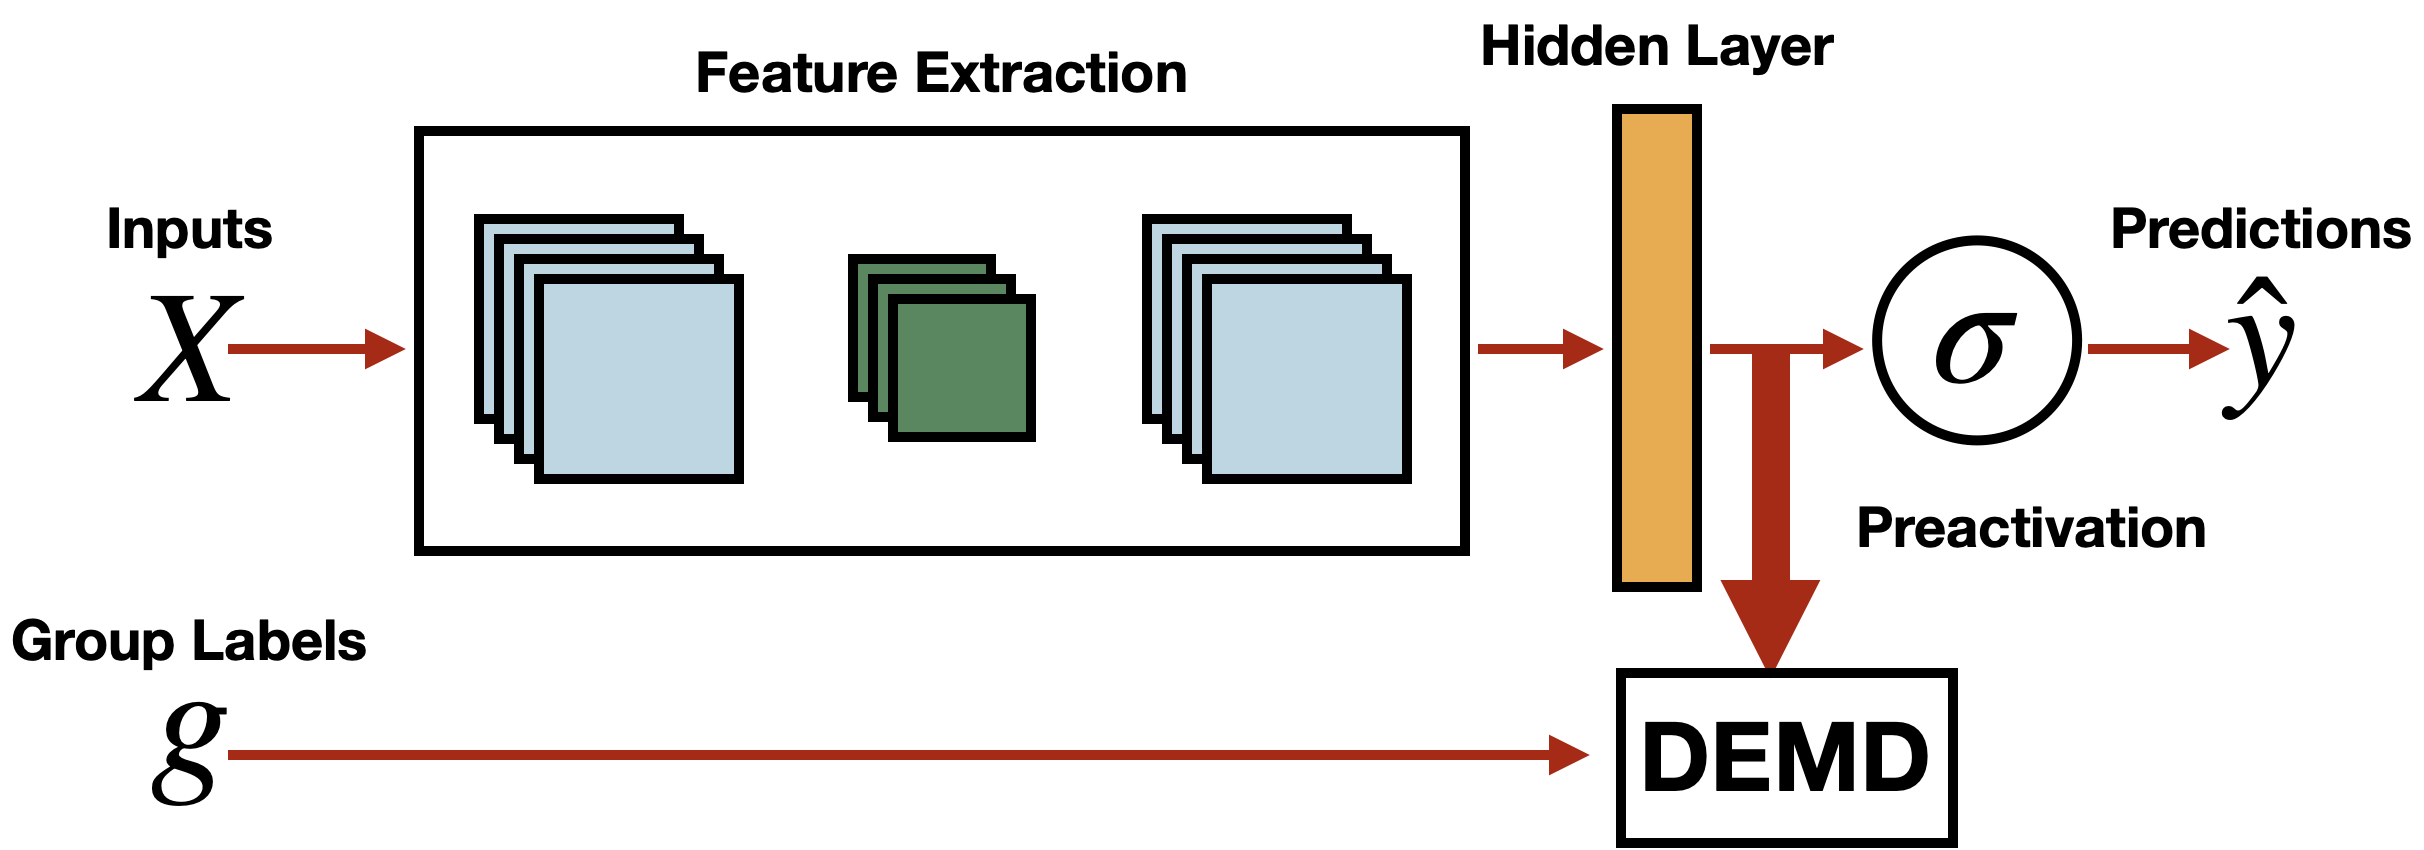
\includegraphics[width=0.55\columnwidth]{6_demd/figs/net_diff_new.png}%
    }% 
    \;
    \includegraphics[width=0.35\columnwidth]{6_demd/figs/Distance_Comparisons.pdf}
    \vspace{-10pt}
    \caption{\footnotesize \label{fig:dists} (Left) DEMD is positioned after the final layer, prior to the activation. Activations are sorted into distributions utilizing group labels provided alongside the input data. Computed distributions are then brought together using our algorithm. (Right) Computation times for direct distance evaluation of EMD-like distances. Existing methods take much more time {\color{blue}(check $y$-axis)} as the number of distributions grow.}
    \vspace{-5pt}
\end{figure}

\section{Experiments}
\label{sec:results}
\vspace{-5pt}
% \subsection{Implementation Details}
% While accounting for dual variables in practice is relatively easy, we may directly take advantage of existing automatically computed gradients from existing software to avoid the bookkeeping and tracking of dual variables entirely. While these gradients may not exactly equal the dual variables, they are directions of descent with respect to our distributions of interest, and are equally sufficient for our purposes.

% Traditional analysis and learning pipelines do not consist of binned distributions, but rather empirical distributions over real-numbered outputs. For this reason it is necessary that we construct a differentiable histogramming operation, that will allow gradients computed with respect to the dEMD measure to flow backwards on a per-sample or per-batch basis. 

% \vishnu{I feel these details are not necessary in the main paper. } Experiments were conducted using NumPy and PyTorch on a Intel(R) Xeon(R) CPU E5-2620 v3 @ 2.40GHz with an Nvidia Titan Xp GPU. 
We evaluate our construction in a number of settings. 
First, we demonstrate the computational speedup associated with evaluating d-MMOT using our algorithm, along with speedups associated with directly computing the gradient.
Next, we compute the construction in a series of neural network tasks associated with ensuring distributional similarity: fairness, invariant representations, and multi-domain matching.
We provide a complete PyTorch Network Module that packages the above differentiable DEMD objective and histogram functions,
and serves as a plug-and-play regularization module. Code is available in the supplement. %\vishnu{One major criticism in the experiments is we don't evaluate in a setting where there are too many distributions to match. }


\subsection{Performance Benchmarks}

Figure \ref{fig:speeds} presents NumPy and Torch instantiations of both forward and backward passes using automatic differentiation and the gradients computed using the dual as in \S\ref{sec:dual}. As expected, the forward (distance computation) times are comparable, but the backwards computation scales poorly with the number of distributions to be updated using automatic differentiation. Our dual setting allows the gradients to simply be read off (based on the forward pass), leading to \textbf{no} additional computation overhead during backpropagation.
\begin{figure}[ht]
    \centering
    \fbox{
    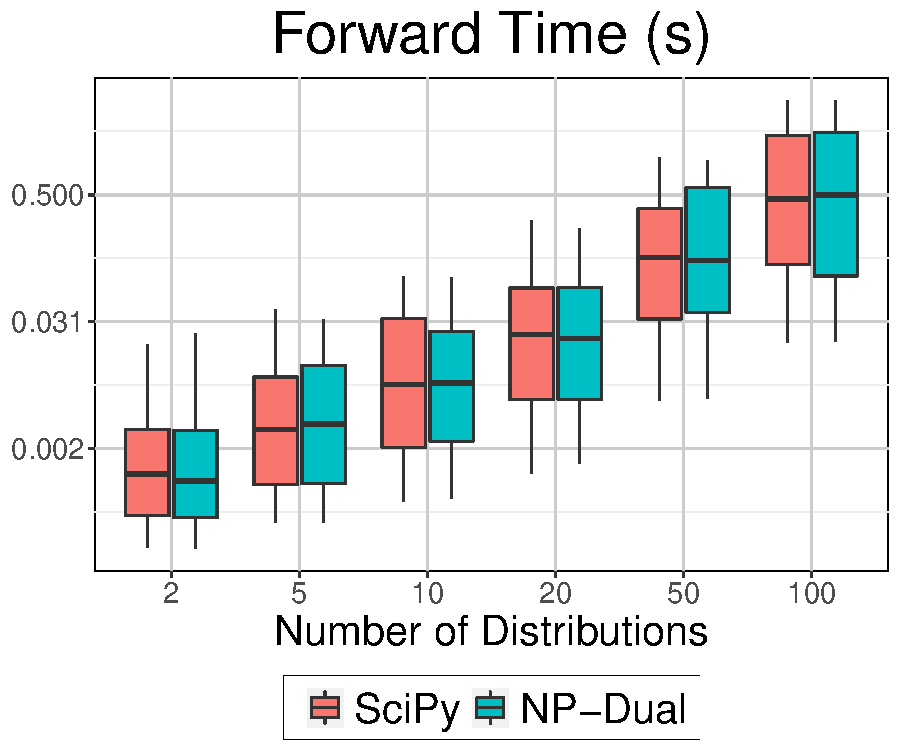
\includegraphics[width=0.22\textwidth]{6_demd/figs/fwbk_new/Numpy_Forwards_10Bins.pdf}
    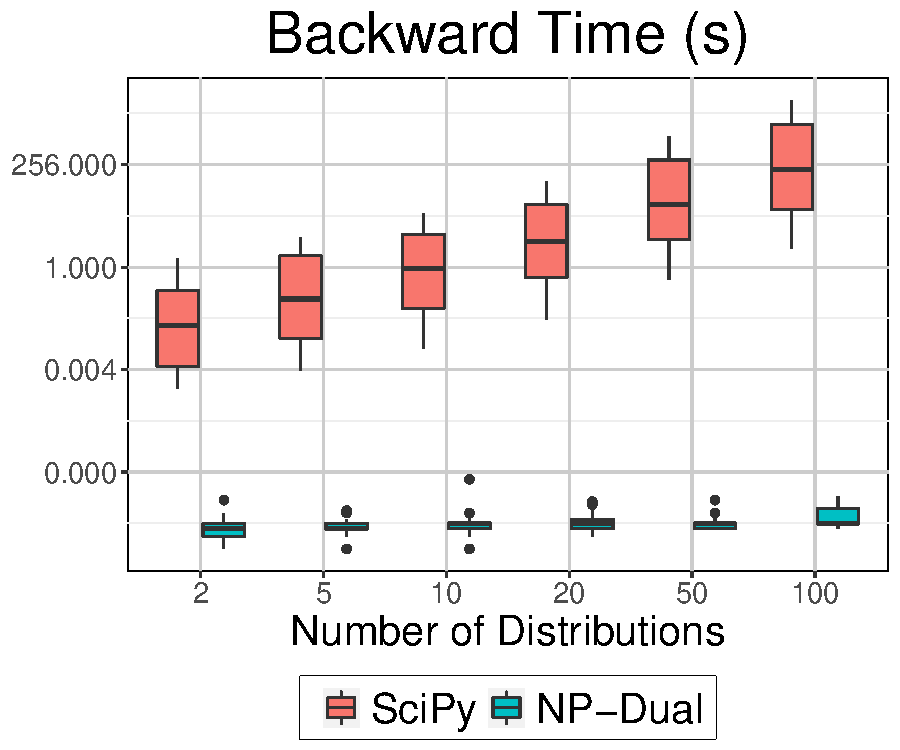
\includegraphics[width=0.22\textwidth]{6_demd/figs/fwbk_new/Numpy_Backward_10Bins.pdf}
    }%
    \;
    \fbox{
    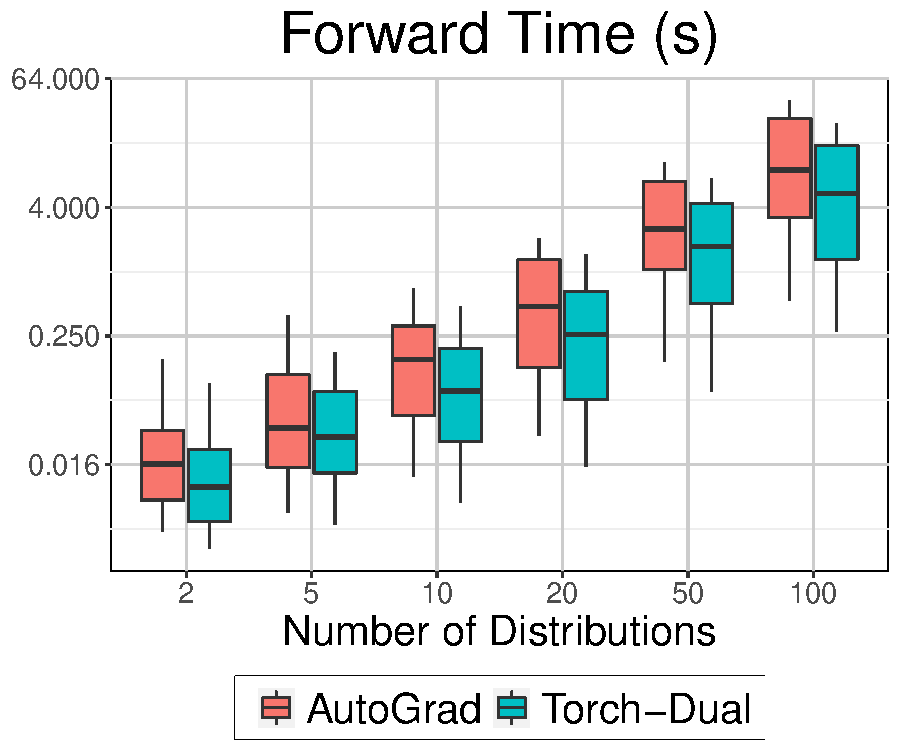
\includegraphics[width=0.22\textwidth]{6_demd/figs/fwbk_new/Torch_Forwards_10Bins.pdf}
    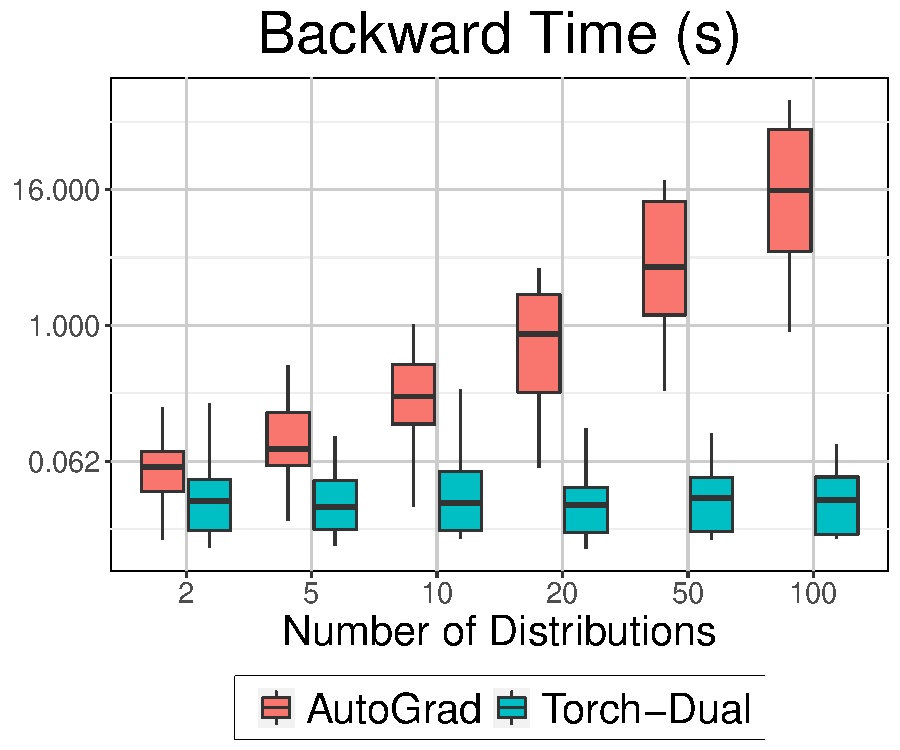
\includegraphics[width=0.22\textwidth]{6_demd/figs/fwbk_new/Torch_Backward_10Bins.pdf}
    }%
    \caption{\footnotesize Forward/Backward Pass Times for 10 Bins with varying number of distributions, averaged over 10 runs. Forward wall-clock times are comparable, regardless of backend ({\em left pair}: NumPy+SciPy; {\em right pair}: PyTorch+AutoGrad). Direct reading of the gradient via the dual leads to significant gains in backward pass times, where automatic differentiation scales poorly with the number of distributions.}
    \label{fig:speeds}
    \vspace{-5pt}
\end{figure}


% \subsection{Comparing Methods for Optimal Transport with Monge Metrics}
We compare our DEMD computation 
%of the Earth Mover's Distance 
to what one may use given existing Optimal Transport methods in Figure \ref{fig:dists} (right). Using standard off-the-shelf methods as a baseline, when the cost is Monge our algorithm provides \textit{significant} speedups in computation time, on the scale of orders of magnitude! Further, if the number of distributions and bins increases, the time-cost for existing methods using more generic LP solvers can become significant, and may become infeasible with generic solutions via CVXPY \citep{diamond2016cvxpy}. 
% Figure \ref{fig:dists} shows the time dependence as the number of distributions grows, with 10 bins. 
We compare our approach to two off-the-shelf implementations of barycenters via the Python Optimal Transport (POT) Library \citep{flamary2021pot}, along with 
directly solving the Earth Mover's problem via CVXPY. 
Even for 10 distributions over 10 bins, CVXPY is unable to allocate the necessary memory using a direct instantiation.

% \begin{figure}
%     \centering
%     \includegraphics[width=0.45\columnwidth]{figs/Distance_Comparisons.pdf}
%     \caption{Times for direct distance computation of EMD-like distances. See text for details.}
%     \label{fig:dists}
% \end{figure}

%% Barycenters doesnt work right now
% \subsection{Common Barycenter Computations and Comparisons}
% -comparing with Cuturi and janati here, working on setup with janati code

% \begin{figure}
%     \centering
%     \includegraphics[width=0.8\columnwidth]{example-image-a}
%     \caption{Comparison of approaches against DEMD over ellipse barycenters.}
%     \label{fig:}
% \end{figure}


%\section{Traditional methods for optimizing fairness: How do we compare?}
% \subsection{Example Applications}
% Here we instantiate the full setting as described in Section \ref{sec:fair}, and compare to existing drop-in regularizers meant to account for fairness. Because our approach operates on the activations prior to classification, we first compare our method using only two bins defined as above or below 0.5, so as to directly mimic the classification metric used in existing setups.

% \subsection{MNIST}
% Using the MNIST handwritten digit dataset, we construct a new classification problem. The distribution of digit size within the frame is typically the same; we augment the dataset with ``small" and ``large" versions of the digits within a single frame, and define a classification problem over determining the size of the digit within the frame. An ideal size classifier in this case should be agnostic to the digit being classified as large or small.

% \begin{figure}
%     \centering
%     \includegraphics[width=0.8\columnwidth]{example-image-b}
%     \caption{Effect of varying DEMD regularization weight, accuracy across groups.}
%     \label{fig:mnist}
% \end{figure}

\subsection{Generalized EM Fairness on Fairness Datasets}
With a viable tool in hand, we move to practical applications in machine learning fairness,
which naturally requires
enforcing closeness in model outputs.
Here, we construct networks with our DEMD regularizer,
where we discretize the final activation output
prior to classification,
and push the distributions of this activation to be similar
among sensitive attributes.

{\bf Data.}
We identify 4 common fairness datasets often used to benchmark
fair machine learning algorithms: (1) the German Credit Dataset \citep{german}, (2) the Adult Income Dataset \citep{uci}, (3) the Communities and Crime Dataset \citep{crime}, and (4) The ACS Income dataset, recently made available as a large, population-level demographic dataset \citep{ding2021retiring} containing as many as nine sensitive attributes. We set up a simple three-layer neural network for classification tasks with the addition of a fairness-type regularizer. We compare our construction with 4 off-the-shelf plug-in regularizers: (1) No regularization, (2) Demographic Parity (DP), (3) Equalized Odds (EO), and (4) a histogrammed barycenter construction. DP and EO regularizers were computed using a PyTorch version of FairLearn \citep{bird2020fairlearn}, and the barycenter version was implemented using POT library (with GPU backend). Because the scale of the regularization term is not directly comparable, we sweep regularization weights and select the best over all measures for a each dataset/regularizer pair. 
We use 10 bins and replicate all experiments over three random seeds.

% The American Census Survey (ACS) has recently made available a large set of demographic data. The original UCI Adult dataset \cite{uci} was curated from this data, however recent work by \cite{ding2021retiring} has identified temporal shifts in demographic data, and recommends using a more recent collection as a baseline when evaluating biases and adjusting for fairness. Part of their contribution includes APIs to directly interface with the data provided by the ACS, and the ability to identify and construct similar problems associated with the original UCI-provided dataset, albeit with updated data. Data for the income prediction task was downloaded from 2018, localized to California. After preprocessing, 195665 samples were split: 75\% training and 25\% validation. Race is the provided group label, which we wish to be agnostic toward over some measure of our output.
{\bf Models.} We set up two model settings with a standard logistic regressor and a 2-layer neural network. We compare three types of plug-in regularizers: (1) Demographic Parity (DP), (2) Equalized Odds (EO), and (3) the Generalized EMD. DP and EO regularizers were computed using a PyTorch implementation of FairLearn \citep{bird2020fairlearn}. 
%Since the scale of the regularization term in our measure is not directly comparable, we sweep over the regularization weights. 

{\bf Results.} In the summary in Table~\ref{tab:fair_results}, models were selected with the largest regularization weight before accuracy dropped significantly. When accuracies are comparable, we see good performance (when minimizing DEMD regularizer) against baseline methods. Notably, when accuracies are similar across methods, minimizing DEMD tends to give better (lower) fairness measures across all datasets.
{\bf Summary:} DEMD on the final network layer helps control multiple fairness measures.


% First we see that sweeps over regularization weights act as expected for our metric, as well as for existing fairness measures. 
% Table~\ref{tab:acsinc2} show results after training with a large range of regularization weights.
% Training models with no regularization leads to significantly different accuracies over race groups within the data, and strong regularization reduces both the EMD distance and traditional fairness measures over the output via demographic parity (DP) and equality of opportunity (EO). Table~\ref{fig:reg_sweep} shows a particular tighter sweep for EMD regularizer with 10 bins used as the discretization level, closer to the region with large swings in the trade-off. Close correspondence with DP and EO measured after thresholding suggests the model may be robust to choices in the selection threshold.
% Validation results for various models and regularization weights on the ACS Income prediction task including demographic parity
% (DP) and equality of opportunity (EO) spreads. In this setting only two bins are used for direct comparison to output-style regularizers.


\begin{table*}[!t] 
	\scriptsize
	\setlength\tabcolsep{3.5pt} % make LaTeX figure out width of inter-column spaces
	\caption{\footnotesize \textbf{Fairness Experiments.} Measures evaluated using standard metrics: maximum Demographic Parity Gap \textbf{(DP)},  maximum Equalized Odds Gap \textbf{(EO)}, and \textbf{(DEMD)}. For all measures, lower values are preferred.  With comparable accuracy, DEMD regularization leads to fairer representations as measured by common metrics. DP and EO measures are scaled by 100 for ease of presentation. Best results shown in bold.}
	\vspace{-10pt}
	\begin{tabular*}{\linewidth}{l *{3}{c}|*{3}{c}|*{3}{c}|*{3}{c}}
		\midrule%\midrule
		& \multicolumn{3}{c}{German} & \multicolumn{3}{c}{Adult} & \multicolumn{3}{c}{Crime}& \multicolumn{3}{c}{ACS-Income} \\
		\cmidrule{2-4} \cmidrule{5-7} \cmidrule{8-10} \cmidrule{11-13}
		& DP & EO & DEMD & DP & EO & DEMD & DP & EO & DEMD & DP & EO & DEMD \\ 
		\midrule
% 		None & 0.180 & 0.134 & 1.694 & 0.382 & 0.446 & 2.858 & 0.351 & 0.306 & 3.556 & 0.365 & 0.251 & 4.778 \\
% DP-Reg. & 0.169 & 0.128 & 1.600 & 0.383 & 0.446 & 2.832 & 0.362 & 0.250 & 3.705 & 0.477 & 0.276 & 5.024 \\
% EO-Reg. & 0.143 & 0.116 & 1.425 & 0.377 & 0.442 & 2.830 & 0.363 & 0.311 & 3.055 & 0.377 & 0.256 & 4.818 \\
% Bary & 0.177 & 0.134 & 1.645 & 0.362 & 0.442 & 2.811 & 0.377 & 0.256 & 2.726 & 0.571 & 0.497 & 4.376 \\
% DEMD & 0.145 & 0.117 & 1.443 & 0.364 & 0.438 & 2.688 & 0.288 & 0.361 & 3.101 & 0.334 & 0.236 & 3.598 \\
None & $17\scriptscriptstyle(5)$ & $11\scriptscriptstyle(2)$ & $1.69\scriptscriptstyle(0.32)$ & $18\scriptscriptstyle(1)$ & $13\scriptscriptstyle(0)$ & $1.69\scriptscriptstyle(0.07)$ & $38\scriptscriptstyle(6)$ & $45\scriptscriptstyle(3)$ & $2.86\scriptscriptstyle(0.38)$ & $37\scriptscriptstyle(1)$ & $25\scriptscriptstyle(0)$ & $4.78\scriptscriptstyle(0.32)$ \\
DP-Reg. & $16\scriptscriptstyle(6)$ & $10\scriptscriptstyle(3)$ & $1.5\scriptscriptstyle(0.26)$ & $17\scriptscriptstyle(1)$ & $13\scriptscriptstyle(1)$ & $1.6\scriptscriptstyle(0.07)$ & $38\scriptscriptstyle(6)$ & $45\scriptscriptstyle(3)$ & $2.83\scriptscriptstyle(0.39)$ & $48\scriptscriptstyle(4)$ & $28\scriptscriptstyle(0)$ & $5.02\scriptscriptstyle(0.31)$ \\
EO-Reg. & $17\scriptscriptstyle(5)$ & $11\scriptscriptstyle(2)$ & $1.69\scriptscriptstyle(0.32)$ & $\textbf{14}\scriptscriptstyle(1)$ & $\textbf{12}\scriptscriptstyle(1)$ & $\textbf{1.43}\scriptscriptstyle(0.07)$ & $38\scriptscriptstyle(5)$ & $\textbf{44}\scriptscriptstyle(3)$ & $2.83\scriptscriptstyle(0.39)$ & $38\scriptscriptstyle(1)$ & $26\scriptscriptstyle(0)$ & $4.82\scriptscriptstyle(0.32)$ \\
Bary-POT & $27\scriptscriptstyle(5)$ & $17\scriptscriptstyle(1)$ & $1.5\scriptscriptstyle(0.21)$ & $18\scriptscriptstyle(1)$ & $13\scriptscriptstyle(0)$ & $1.64\scriptscriptstyle(0.07)$ & $\textbf{36}\scriptscriptstyle(5)$ & $\textbf{44}\scriptscriptstyle(4)$ & $2.81\scriptscriptstyle(0.3)$ & $57\scriptscriptstyle(37)$ & $50\scriptscriptstyle(44)$ & $4.38\scriptscriptstyle(0.16)$ \\
DEMD (ours) & $\textbf{14}\scriptscriptstyle(7)$ & $\textbf{9}\scriptscriptstyle(4)$ & $\textbf{1.41}\scriptscriptstyle(0.35)$ & $15\scriptscriptstyle(1)$ & $\textbf{12}\scriptscriptstyle(1)$ & $1.44\scriptscriptstyle(0.08)$ & $\textbf{36}\scriptscriptstyle(6)$ & $\textbf{44}\scriptscriptstyle(3)$ & $\textbf{2.69}\scriptscriptstyle(0.44)$ & $\textbf{33}\scriptscriptstyle(0)$ & $\textbf{24}\scriptscriptstyle(0)$ & $\textbf{3.6}\scriptscriptstyle(0.29)$ \\
		\midrule%\midrule
	\end{tabular*}
	\label{tab:fair_results}
	%\vspace{-20pt}
\end{table*} 

\subsection{Harmonization for Invariant Representations}
Having evaluated the use of the DEMD layer to constrain the neural network for  fairness measures, we will now move to a more general problem of deriving invariant representations from the datasets. Here, invariance is sought in regard to the sensitive attributes. Recent works \citep{equivar} on invariant representation learning propose leveraging an encoder-decoder architectures to map the dataset features to latent space representations. The latent space representations are penalized to match or harmonize the distributions across several groups in the dataset. In contrast to the previous section, the goal here is to identify a good mapping in the latent space that is devoid of any group-related information in the dataset.  Consequently, our evaluation metrics test if the latent representations have a lower value of (i) ADV, adversarial measure and (ii) MMD, maximum mean discrepancy measure. The measure ADV tests to what extent can a separate neural network predict the group information from the latent features. Alternatively, the MMD scores measure the distance between the probability distributions across groups. Prior works such as \cite{zemel} and \cite{cai} optimize each of these measures separately. Our experiments (Table~\ref{tab:harm_results}) show the DEMD layer performs competitively with the baselines when applied on the latent space. Interestingly, these performance gains come despite not directly optimizing the harmonization measures, in contrast to baselines, which require several practical adjustments (batch variants and secondary neural networks).
\textbf{Summary}: DEMD as an intermediate layer can be used to derive invariant representations efficiently.
% \vishnu{Need to convey a message that the baseline directly optimizes for the ADV and MMD measures. Our although doesn't directly optimizes these measures, still achieves competitive values on them. }
%Due to skewness amongst the groups, ROC-AUC is used to report the ADV measure on German dataset.
\begin{table*}[!t] 
	\scriptsize
	\setlength\tabcolsep{2.25pt} % make LaTeX figure out width of inter-column spaces
	\caption{\footnotesize \textbf{Harmonization Experiments.} Evaluations conducted along three metrics, Accuracy \textbf{(ACC)}, Adversarial measure \textbf{(ADV)} and Maximum Mean Discrepancy \textbf{(MMD)}. A lower value $\downarrow$ of ADV and MMD indicate successful harmonization across the different groups. A higher ACC with a small drop from baseline is preferred. }
	\vspace{-10pt}
	\begin{tabular*}{\linewidth}{l *{3}{c}|*{3}{c}|*{3}{c}|*{3}{c}}
		\midrule%\midrule
		& \multicolumn{3}{c}{German} & \multicolumn{3}{c}{Adult} & \multicolumn{3}{c}{Crime}& \multicolumn{3}{c}{ACS-Income} \\
		\cmidrule{2-4} \cmidrule{5-7} \cmidrule{8-10} \cmidrule{11-13}
		& ACC $\uparrow$ & ADV $\downarrow$ & MMD $\downarrow$ & ACC $\uparrow$ & ADV $\downarrow$ & MMD $\downarrow$ & ACC $\uparrow$ & ADV $\downarrow$ & MMD $\downarrow$ & ACC $\uparrow$ & ADV $\downarrow$  & MMD $\downarrow$ \\ 
		\midrule
		None & $74\scriptscriptstyle(0.9)$ & $93\scriptscriptstyle(1.3)$ & $7.7\scriptscriptstyle(0.8)$ & $84\scriptscriptstyle(0.1)$ & $83\scriptscriptstyle(0.1)$ & $9.8\scriptscriptstyle(0.3)$ & $85\scriptscriptstyle(0.2)$ & $77\scriptscriptstyle(0.5)$ & $14\scriptscriptstyle(0.1)$ & $78\scriptscriptstyle(0.1)$ & $98\scriptscriptstyle(0.7)$ & $160\scriptscriptstyle(2)$ \\
		\cite{zemel} & $73\scriptscriptstyle(1.5)$ & $92\scriptscriptstyle(1.3)$ & $1.5\scriptscriptstyle(0.3)$ & $84\scriptscriptstyle(0.1)$ & $83\scriptscriptstyle(0.1)$ & $3.1\scriptscriptstyle(0.3)$ & $85\scriptscriptstyle(0.5)$ & $76\scriptscriptstyle(1.6)$ & $12\scriptscriptstyle(1.0)$ & $78\scriptscriptstyle(0.1)$ & $97\scriptscriptstyle(0.5)$ & $17\scriptscriptstyle(1.2)$ \\
		\cite{cai} & $76\scriptscriptstyle(1.3)$ & $93\scriptscriptstyle(0.6)$ & $1.2\scriptscriptstyle(0.2)$ & $84\scriptscriptstyle(0.04)$ & $81\scriptscriptstyle(0.7)$ & $4.2\scriptscriptstyle(2.4)$ & $85\scriptscriptstyle(0.2)$ & $76\scriptscriptstyle(0.7)$ & $15\scriptscriptstyle(0.6)$ & $78\scriptscriptstyle(0.1)$ & $94\scriptscriptstyle(5.6)$ & $99\scriptscriptstyle(2.9)$ \\
		DEMD (ours) & $74\scriptscriptstyle(1.1)$ & $93\scriptscriptstyle(0.4)$ & $2.1\scriptscriptstyle(0.4)$ & $84\scriptscriptstyle(0.03)$ & $82\scriptscriptstyle(0.2)$ & $5.3\scriptscriptstyle(1.4)$ & $83\scriptscriptstyle(0.3)$ & $72\scriptscriptstyle(1.0)$ & $7.1\scriptscriptstyle(1.0)$ & $77\scriptscriptstyle(0.4)$ & $96\scriptscriptstyle(0.5)$ & $26\scriptscriptstyle(3.9)$ \\
		\midrule
	\end{tabular*}
	\label{tab:harm_results}
	%\vspace{-5pt}
\end{table*} 

% \scriptscriptstyle(XXX)
%%%% This is a copy of the table from vishnu, needs to be formatted properly
% \begin{table*}[!t] 
% 	\footnotesize
% 	\captionsetup{justification=centering} 
% 	\setlength\tabcolsep{0pt} % make LaTeX figure out width of inter-column spaces
% 	\caption*{$\boldsymbol{{\Delta}_{Eq}}:$  Equivariance Gap, $\boldsymbol{Adv}:$ Adversarial Test Accuracy, $\boldsymbol{\mathcal{M}}:$ Test  $\mathcal{MMD}$ measure, $\boldsymbol{\mathcal{ACC}}:$ Test prediction accuracy\\
% 		$\uparrow$: Higher Value is preferred, $\downarrow$: Lower Value is preferred}
% 	\vspace{-4mm}
% 	\begin{tabular*}{\linewidth}{l @{\extracolsep{\fill}}
% 			*{24}{S[table-format=3.0]}}
% 		\midrule\midrule
% 		& \multicolumn{4}{c}{German} & \multicolumn{4}{c}{Adult} & \multicolumn{4}{c}{ADNI}& \multicolumn{4}{c}{ADCP} \\
% 		\cmidrule{2-5} \cmidrule{6-9} \cmidrule{10-13} \cmidrule{14-17}
% 		& {${\Delta}_{Eq}$ $\uparrow$} & {$Adv$ $\downarrow$} & {$\newsym{M}$ $\downarrow$} & \cellcolor{gray!25}{$\mathcal{ACC}$ $\uparrow$} & {${\Delta}_{Eq}$ $\uparrow$} & {$Adv$ $\downarrow$} & {$\newsym{M}$ $\downarrow$} & \cellcolor{gray!25}{$\mathcal{ACC}$ $\uparrow$} & {${\Delta}_{Eq}$ $\uparrow$} & {$Adv$ $\downarrow$} & {$\newsym{M}$ $\downarrow$} & \cellcolor{gray!25}{$\mathcal{ACC}$ $\uparrow$} & {${\Delta}_{Eq}$ $\uparrow$} & {$Adv$ $\downarrow$} & {$\newsym{M}$ $\downarrow$} & \cellcolor{gray!25}{$\mathcal{ACC}$ $\uparrow$}  \\ 
% 		\midrule\midrule
% 		Na\"ive & {$4.6{\scriptscriptstyle(0.7)}$ } &  {$0.62{\scriptscriptstyle(0.03)}$ }  &  {$7.7{\scriptscriptstyle(0.8)}$}  &  \cellcolor{gray!25}{$74{\scriptscriptstyle(0.9)}$}  &  {$3.4{\scriptscriptstyle(0.7)}$}  &  {$83{\scriptscriptstyle(0.1)}$}  &  {$9.8{\scriptscriptstyle(0.3)}$}  &  \cellcolor{gray!25}{$84{\scriptscriptstyle(0.1)}$}  &  {$3.1{\scriptscriptstyle(1.0)}$}  &  {$59{\scriptscriptstyle(2.9)}$}  &  {$27{\scriptscriptstyle(1.6)}$}  &  \cellcolor{gray!25}{$80{\scriptscriptstyle(2.6)}$} &  {$4.1{\scriptscriptstyle(0.9)}$} &  {$49{\scriptscriptstyle(8.4)}$} &  {$90{\scriptscriptstyle(8.7)}$} &  \cellcolor{gray!25}{$83{\scriptscriptstyle(4.4)}$}    \\
% 		MMD \cite{li2014learning}  & {$4.5{\scriptscriptstyle(1.0)}$ }&  {$0.66{\scriptscriptstyle(0.04)}$}  &  {$1.5{\scriptscriptstyle(0.3)}$}  &  \cellcolor{gray!25}{$73{\scriptscriptstyle(1.5)}$}  &  {$3.4{\scriptscriptstyle(0.9)}$}  &  {$83{\scriptscriptstyle(0.1)}$}  &  {$3.1{\scriptscriptstyle(0.3)}$}  &  \cellcolor{gray!25}{$84{\scriptscriptstyle(0.1)}$} &  {$3.1{\scriptscriptstyle(1.0)}$}  &  {$59{\scriptscriptstyle(3.3)}$}  &  {$27{\scriptscriptstyle(1.7)}$}  &  \cellcolor{gray!25}{$80{\scriptscriptstyle(2.6)}$}   &  {$3.6{\scriptscriptstyle(1.0)}$} &  {$49{\scriptscriptstyle(11.9)}$} &  {$86{\scriptscriptstyle(11.0)}$} &  \cellcolor{gray!25}{$84{\scriptscriptstyle(6.5)}$}  \\ 
% 		CAI \cite{NIPS2017_8cb22bdd} & {$1.9{\scriptscriptstyle(0.6)}$ }&  {$0.65{\scriptscriptstyle(0.01)}$}  &  {$1.2{\scriptscriptstyle(0.2)}$}  &  \cellcolor{gray!25}{$76{\scriptscriptstyle(1.3)}$}  &  {$0.1{\scriptscriptstyle(0.0)}$}  &  {$81{\scriptscriptstyle(0.7)}$}  &  {$4.2{\scriptscriptstyle(2.4)}$}  &  \cellcolor{gray!25}{$84{\scriptscriptstyle(0.04)}$}  &  {$2.4{\scriptscriptstyle(0.7)}$}  &  {$61{\scriptscriptstyle(2.1)}$}  &  {$27{\scriptscriptstyle(1.5)}$}  &  \cellcolor{gray!25}{$74{\scriptscriptstyle(3.6)}$}   &  {$2.8{\scriptscriptstyle(1.6)}$} &  {$56{\scriptscriptstyle(6.9)}$} &  {$85{\scriptscriptstyle(12.3)}$} &  \cellcolor{gray!25}{$82{\scriptscriptstyle(5.1)}$} \\ 
% 		SS \cite{zhou2018statistical} & {$3.8{\scriptscriptstyle(0.5)}$ }&  {$0.70{\scriptscriptstyle(0.07)}$}  &  {$1.5{\scriptscriptstyle(0.6)}$}  &  \cellcolor{gray!25}{$76{\scriptscriptstyle(0.9)}$}  &  {$2.8{\scriptscriptstyle(0.5)}$}  &  {$83{\scriptscriptstyle(0.2)}$}  &  {$1.5{\scriptscriptstyle(0.2)}$}  &  \cellcolor{gray!25}{$84{\scriptscriptstyle(0.1)}$}  &  {$3.7{\scriptscriptstyle(0.5)}$}  &  {$57{\scriptscriptstyle(2.1)}$}  &  {$26{\scriptscriptstyle(1.6)}$}  &  \cellcolor{gray!25}{$81{\scriptscriptstyle(3.7)}$}   &  {$3.4{\scriptscriptstyle(1.3)}$} &  {$51{\scriptscriptstyle(6.7)}$} &  {$88{\scriptscriptstyle(14.6)}$} &  \cellcolor{gray!25}{$82{\scriptscriptstyle(3.5)}$} \\ 	
% 		RM \cite{motiian2017unified} & {$3.4{\scriptscriptstyle(0.4)}$ }&  {$0.66{\scriptscriptstyle(0.04)}$}  &  {$7.5{\scriptscriptstyle(0.9)}$}  &  \cellcolor{gray!25}{$74{\scriptscriptstyle(2.1)}$}  &  {$0.8{\scriptscriptstyle(0.1)}$}  &  {$82{\scriptscriptstyle(0.4)}$}  &  {$4.8{\scriptscriptstyle(0.7)}$}  &  \cellcolor{gray!25}{$84{\scriptscriptstyle(0.3)}$}  &  {$0.8{\scriptscriptstyle(0.9)}$}  &  {$52{\scriptscriptstyle(5.4)}$}  &  {$22{\scriptscriptstyle(0.6)}$}  &  \cellcolor{gray!25}{$78{\scriptscriptstyle(3.8)}$}   &  {$0.4{\scriptscriptstyle(0.5)}$} &  {$40{\scriptscriptstyle(4.7)}$} &  {$77{\scriptscriptstyle(13.8)}$} &  \cellcolor{gray!25}{$84{\scriptscriptstyle(5.3)}$} \\ 	
% 		Ours & {$\boldsymbol{6.4{\scriptscriptstyle(0.6)}}$ } &  {$\boldsymbol{0.54{\scriptscriptstyle(0.01)}}$}  &  {$2.7{\scriptscriptstyle(0.6)}$}  &  \cellcolor{gray!25}{$75{\scriptscriptstyle(3.3)}$}  &  {$\boldsymbol{5.3{\scriptscriptstyle(0.9)}}$}  &  {$\boldsymbol{75{\scriptscriptstyle(1.4)}}$}  &  {$7.1{\scriptscriptstyle(0.6)}$}  &  \cellcolor{gray!25}{$83{\scriptscriptstyle(0.1)}$} &  {$\boldsymbol{5.1{\scriptscriptstyle(1.2)}}$}  &  {$\boldsymbol{50{\scriptscriptstyle(4.2)}}$}  &  {$\boldsymbol{16{\scriptscriptstyle(7.2)}}$}  &  \cellcolor{gray!25}{$77{\scriptscriptstyle(4.8)}$} &  {$\boldsymbol{7.5{\scriptscriptstyle(1.2)}}$} &  {$49{\scriptscriptstyle(7.3)}$} &  {$\boldsymbol{70{\scriptscriptstyle(22.3)}}$} &  \cellcolor{gray!25}{$81{\scriptscriptstyle(1.8)}$}  \\ 
% 		\midrule\midrule
% 	\end{tabular*} 
% 	\captionsetup{justification=justified} 
% 	\caption{ \footnotesize  \textbf{Quantitative Results.} We show Mean(Std) results over multiple run. For our baselines, we consider a \textbf{Na\"ive} encoder-decoder model, learning  representations via minimizing the \textbf{MMD} criterion \cite{li2014learning} and Adversarial training \cite{NIPS2017_8cb22bdd}, termed as \textbf{CAI}. We also compare against Sub-sampling (\textbf{SS}) \cite{zhou2018statistical} that minimizes the MMD criterion separately for every age group, and  the RandMatch (\textbf{RM}) \cite{motiian2017unified} baseline that generates matching input pairs based on the Age and target label values. The SS and RM baselines discard subset of samples if a match across sites is not available. The measure $Adv$ represents the adversarial test accuracy except for the German dataset where ROC-AUC is used due to high degree of skew in the data.  } 
% 	\label{tab:results}
% 	\vspace{-0.3in}
% \end{table*} 
\subsection{Multi-domain Image Translation}
%\glenn{Its not totally clear how we are suing DEMD here. Is it that we are regularizing the feature distribution in a new domain to be close to a new domain, right?, we need to clarify this with a sentence or two}  
We apply our construction to a recent multi-marginal GAN framing of multi-domain image translation.
With the goal of learning a mapping for a source image to multiple target domains, a focal point of recent literature has been to reduce the computational requirements of training individual models for each target, and learn a concurrent matching problem over a number of shared parameters or networks. MWGAN \citep{cao2019multi} set up a Multiple Marginal Matching problem in this context.
Extending upon their key observation that inter-domain constraints can be measured via the gradients for each domain,
we instantiate our DEMD layer over the gradient norms computed for each sample in a batch per group.
Specifically, DEMD minimizes the differences between the distributions over the gradient norms across all target domains.
% \jeff{at this spot it works to put a word on why DEMD going to be useful.  also emphasize that DEMD is used as a drop-in replacement module}
% Results are in agreement with results using MWGAN.
Using a weight of 100 for both regularizers,
we observe similar performance when compared 
to the original MWGAN construction.
In Figure~\ref{fig:mwgan} we show a few samples generated over an image translation task on the CelebA dataset.
Here, we aim to translate original dataset images to ones with specific target attributes.
\textbf{Summary:} Multi-domain image translation can be conducted by adding a DEMD layer in the native GAN construction. 

% \begin{figure}
%     \centering
%     % 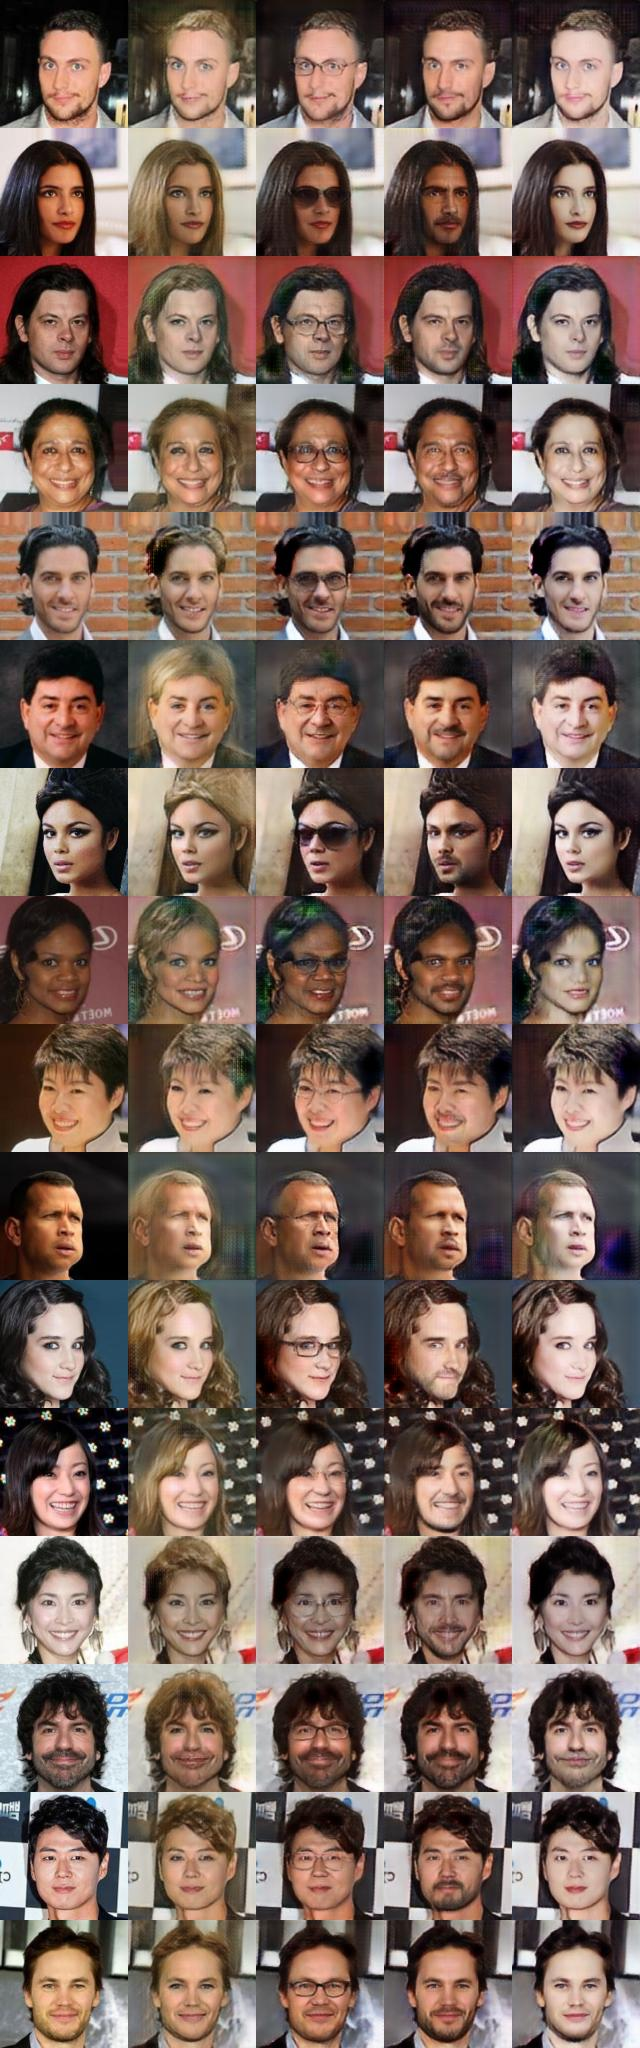
\includegraphics[width=0.49\linewidth,trim={0 59cm 0 0},clip]{figs/mwgan/baseline_050000-images.jpg}
%     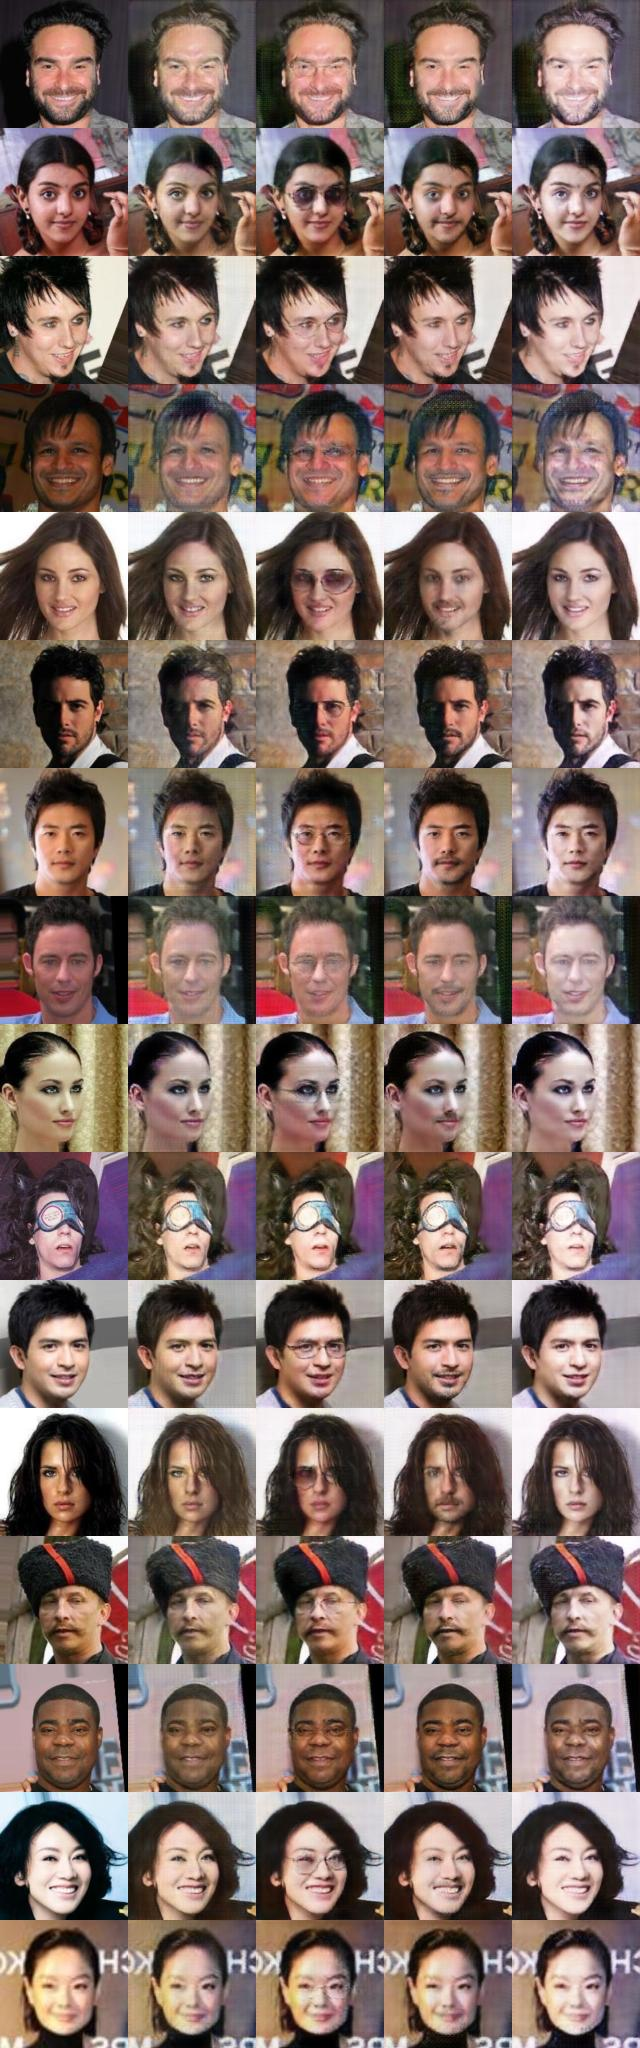
\includegraphics[width=0.49\linewidth,trim={0 58.7cm 0 0},clip]{figs/mwgan/046500-images.jpg}
%     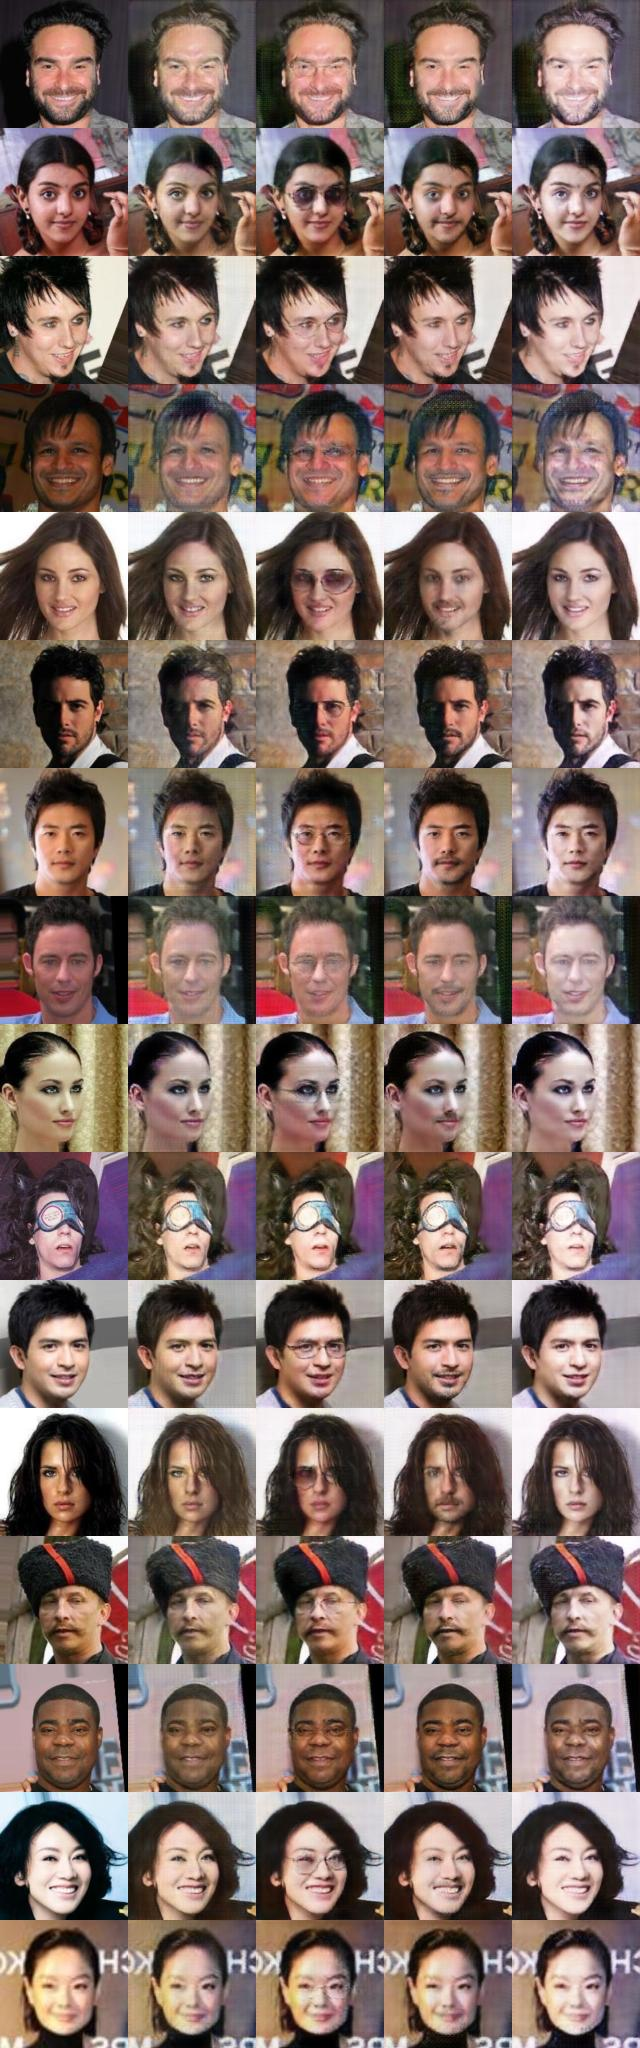
\includegraphics[width=0.49\linewidth,trim={0 0 0 58.7cm},clip]{figs/mwgan/046500-images.jpg}
%     % 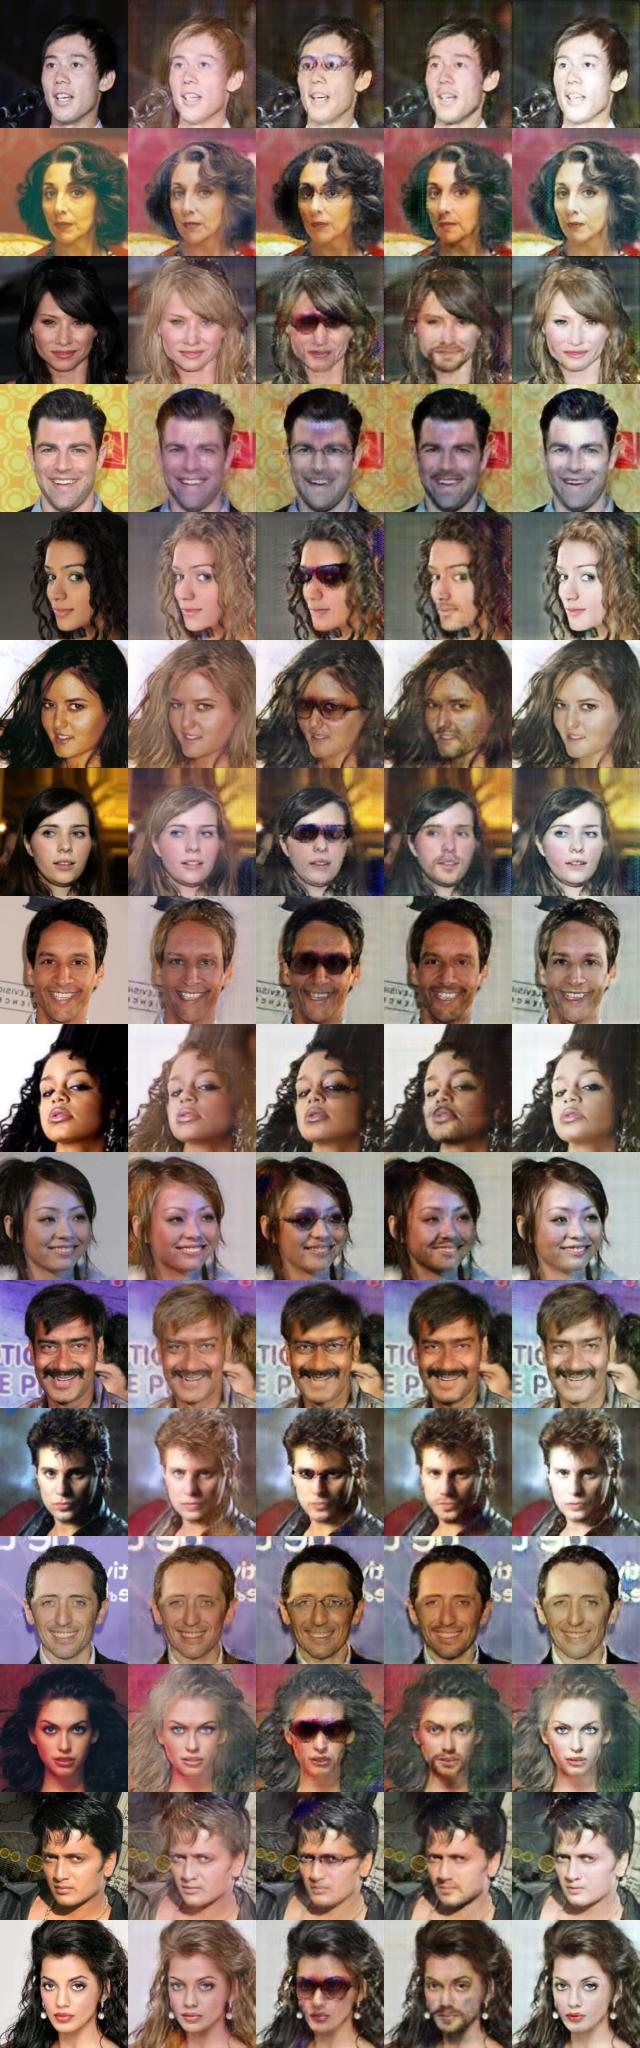
\includegraphics[width=0.49\linewidth,trim={0 63.5cm 0 0},clip]{figs/mwgan/demd_050000-images.jpg}
%     % 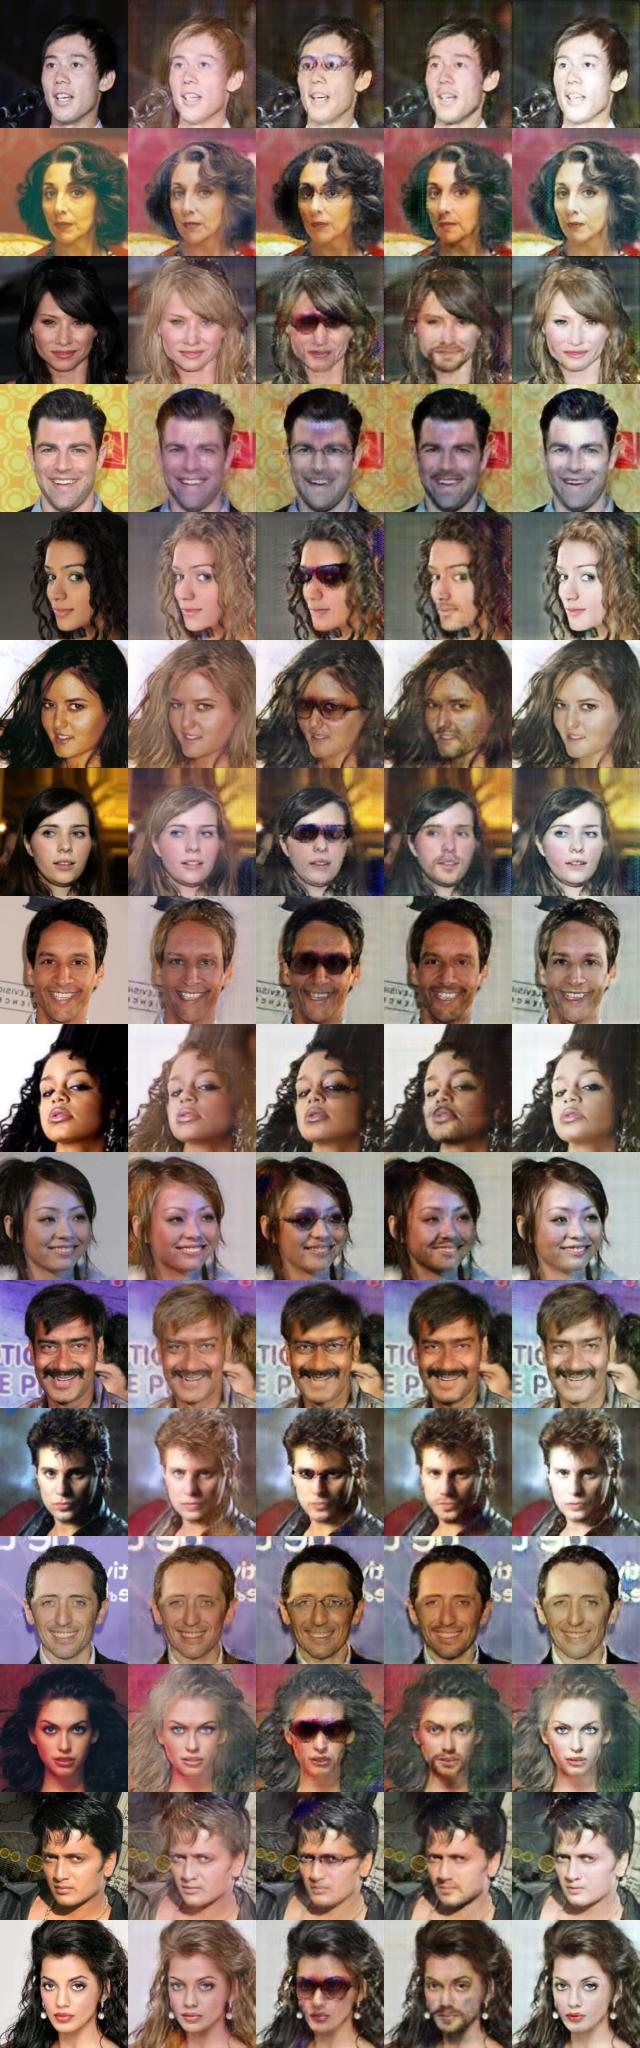
\includegraphics[width=0.49\linewidth,trim={0 63.5cm 0 0},clip]{figs/mwgan/demd_050000-images.jpg}
%     \caption{\footnotesize Six MWGAN+DEMD CelebA image translation results. Each row corresponds to a random sample in the validation set. The leftmost image is the original source image, and sequential columns represent translations to (1) Blonde Hair, (2) Glasses, (3) Mustache, and (4) Pale Skin.\ronak{put labels on top of images? add bar separating original and targets?}}
%     \label{fig:mwgan}
% \end{figure}

\begin{figure*}[t]
    \centering
    \scriptsize
    	Original \quad\; Blond Hair \quad\; Glasses \quad\; Moustache \quad\; Pale Skin \quad\quad Original \quad\; Blond Hair \quad\; Glasses \quad\; Moustache \quad\; Pale Skin \\
    	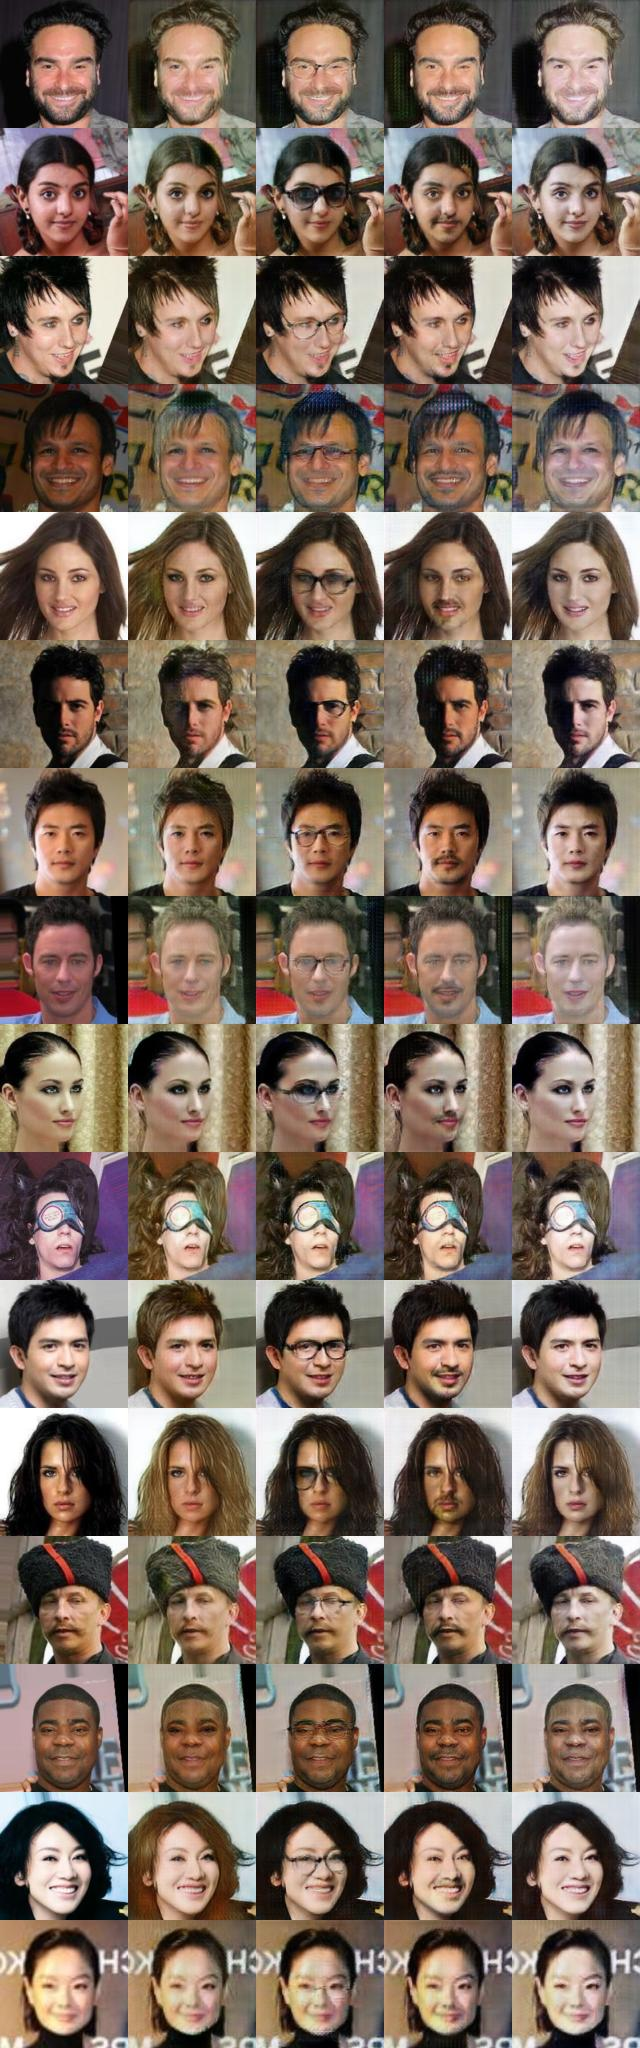
\includegraphics[width=0.49\linewidth,trim={0 58.7cm 0 0},clip]{6_demd/figs/mwgan/069500-images.jpg} 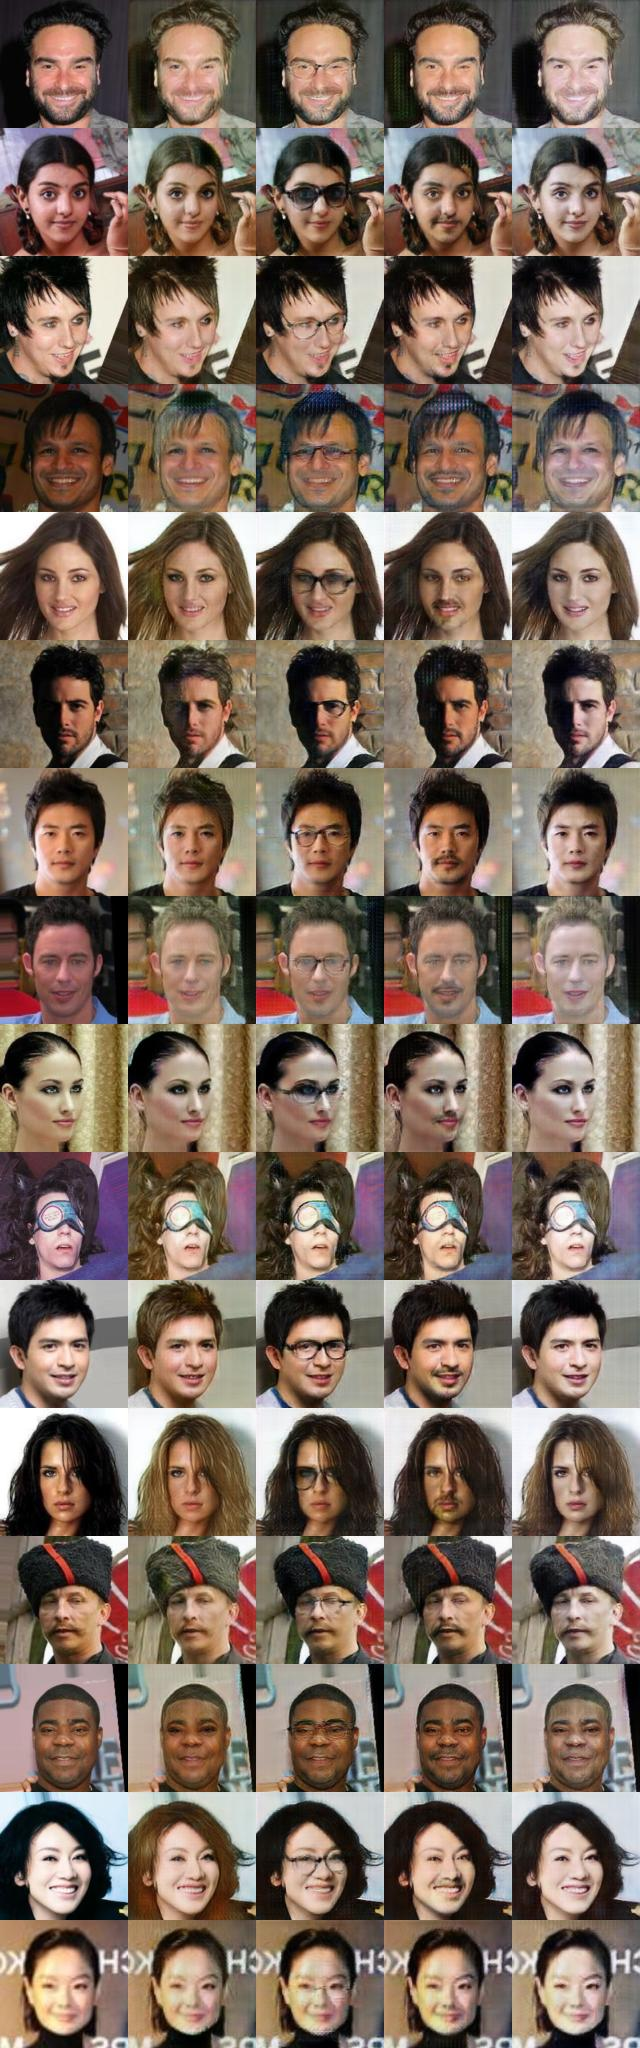
\includegraphics[width=0.49\linewidth,trim={0 0 0 58.7cm},clip]{6_demd/figs/mwgan/069500-images.jpg}
    \caption{Six MWGAN+DEMD CelebA image translation results. Each row corresponds to a random sample in the validation set. The leftmost image is the original source image, and sequential columns represent translations to (1) Blonde Hair, (2) Glasses, (3) Moustache, and (4) Pale Skin. Using DEMD as a relaxation to the Multiple Marginal Matching problem facilitates high quality images translation. For more results see Appendix~\ref{sec:app-mwgan}. }
    \label{fig:mwgan}
\end{figure*}


%%%%%%%%%%%%%%%%%%%%%%% OLD stuff
%%%%%%%%%%%%%%%%%%%%%%% OLD stuff
%%%%%%%%%%%%%%%%%%%%%%% OLD stuff
%%%%%%%%%%%%%%%%%%%%%%% OLD stuff



% \begin{table*}[!t] 
% 	\scriptsize
% 	\setlength\tabcolsep{4pt} % make LaTeX figure out width of inter-column spaces
% 	\caption{\footnotesize Fairness validation results, higher accuracy is better, Lower Fairness measures are better. Higher accuracies \textbf{(ACC)} with lower measures of max Demographic Parity Gap \textbf{(|DP|)},  Equalized Odds Gap \textbf{(|EO|)}, and \textbf{(DEMD)}. \vishnu{Other methods minimize DEMD better than DEMD algorithm itself? Kinda mixed message} \vishnu{Accuracy values should not be in bold. Infact, separate color needs to be used for accuracy column. The idea is that upto 2-4\% drop in accuracy is permissible as long as the fairness measures improve.} \vishnu{Accuracy values are different from this table to the next one! accuracy is kinda redundant information. Best if avoided or moved to the supplement}}
% 	\begin{tabular*}{\linewidth}{l *{3}{c}|*{3}{c}|*{3}{c}|*{3}{c}}
% 		\midrule%\midrule
% 		& \multicolumn{3}{c}{German} & \multicolumn{3}{c}{Adult} & \multicolumn{3}{c}{Crime}& \multicolumn{3}{c}{ACS-Employ} \\
% 		\cmidrule{2-4} \cmidrule{5-7} \cmidrule{8-10} \cmidrule{11-13}
% 		& ACC & |DP| & |EO| & DEMD & ACC  & |DP| & |EO| & DEMD & ACC & |DP| & |EO| & DEMD & ACC & |DP| & |EO| & DEMD \\ 
% 		\midrule
% 		None & 0.180 & 0.134 & 1.694 & 0.382 & 0.446 & 2.858 & 0.351 & 0.306 & 3.556 & 0.365 & 0.251 & 4.778 \\
% DP-Reg. & 0.169 & 0.128 & 1.600 & 0.383 & 0.446 & 2.832 & 0.362 & 0.250 & 3.705 & 0.477 & 0.276 & 5.024 \\
% EO-Reg. & 0.143 & 0.116 & 1.425 & 0.377 & 0.442 & 2.830 & 0.363 & 0.311 & 3.055 & 0.377 & 0.256 & 4.818 \\
% Bary & 0.177 & 0.134 & 1.645 & 0.362 & 0.442 & 2.811 & 0.377 & 0.256 & 2.726 & 0.571 & 0.497 & 4.376 \\
% DEMD & 0.145 & 0.117 & 1.443 & 0.364 & 0.438 & 2.688 & 0.288 & 0.361 & 3.101 & 0.334 & 0.236 & 3.598 \\
% % 		None & 0.77 & 0.17 & 0.11 & 1.69 & \textbf{0.84} & 0.18 & 0.13 & 1.69 & \textbf{0.84} & 0.38 & 0.45 & 2.86 & \textbf{0.80} & 0.35 & 0.31 & 3.56 \\
% % DP-Reg. & 0.77 & 0.16 & 0.10 & 1.50 & \textbf{0.84} & 0.17 & 0.13 & 1.60 & 0.83 & 0.37 & 0.44 & 2.65 & 0.79 & 0.36 & \textbf{0.25} & 3.71 \\
% % EO-Reg. & 0.75 & 0.20 & 0.11 & 1.59 & \textbf{0.84} & 0.14 & \textbf{0.12} & 1.43 & 0.83 & \textbf{0.35} & \textbf{0.43} & 2.54 & 0.79 & 0.53 & 0.36 & 3.06 \\
% % Bary & \textbf{0.79} & 0.27 & 0.17 & 1.50 & 0.81 & \textbf{0.13} & 0.14 & \textbf{0.99} & 0.81 & \textbf{0.35} & 0.44 & \textbf{2.61} & 0.79 & 0.38 & 0.26 & \textbf{2.73} \\
% % DEMD & 0.77 & \textbf{0.14} & \textbf{0.09} & \textbf{1.41} & \textbf{0.84} & 0.15 & \textbf{0.12} & 1.44 & 0.83 & 0.36 & 0.44 & 2.69 & \textbf{0.80} & \textbf{0.29} & 0.36 & 3.10 \\
% % 		None & XXYY & XXYY & XXYY & XXYY  & XXYY & XXYY & XXYY & XXYY & XXYY & XXYY & XXYY & XXYY & XXYY & XXYY & XXYY & XXYY \\
% % 		DP & XXYY & XXYY & XXYY & XXYY & XXYY & XXYY & XXYY & XXYY & XXYY & XXYY & XXYY & XXYY & XXYY & XXYY & XXYY & XXYY \\
% % 		EO & XXYY & XXYY & XXYY & XXYY & XXYY & XXYY & XXYY & XXYY & XXYY & XXYY & XXYY & XXYY & XXYY & XXYY & XXYY & XXYY \\
% % 		Bary & XXYY & XXYY & XXYY & XXYY & XXYY & XXYY & XXYY & XXYY & XXYY & XXYY & XXYY & XXYY & XXYY & XXYY & XXYY & XXYY \\
% % 		DEMD & XXYY & XXYY & XXYY & XXYY & XXYY & XXYY & XXYY & XXYY & XXYY & XXYY & XXYY & XXYY & XXYY & XXYY & XXYY & XXYY \\
% 		\midrule%\midrule
% 	\end{tabular*}
% 	\label{tab:fair_results}
% \end{table*} 

% \begin{table}[]
%     \centering
%     \begin{tabular}{c|cccc}
%         \toprule
%         $\lambda_{reg}$ & Acc & DP Gap & EO Gap & EMD \\
%         \midrule
%         0.00 & 0.776 & 0.665 & 0.723 & 3.352 \\
%         0.01 & 0.776 & 0.670 & 0.726 & 3.050 \\
%         0.02 & 0.776 & 0.474 & 0.527 & 2.317 \\
%         0.03 & 0.773 & 0.485 & 0.531 & 1.965 \\
%         0.04 & 0.763 & 0.506 & 0.540 & 1.575 \\
%         0.05 & 0.738 & 0.339 & 0.356 & 1.149 \\
%         0.06 & 0.670 & 0.178 & 0.200 & 0.662 \\
%         0.07 & 0.594 & 0.006 & 0.005 & 0.372 \\
%         0.08 & 0.590 & 0.000 & 0.000 & 0.031 \\
%         0.09 & 0.590 & 0.000 & 0.000 & 0.000 \\
%         0.10 & 0.590 & 0.000 & 0.000 & 0.000 \\\bottomrule
%     \end{tabular}
%     \caption{Outcome measures as a function of regularization parameter when our EMD regularizer is used.}
%     \label{tab:reg_sweep}
% \end{table}

% \begin{figure}
%     \centering
%     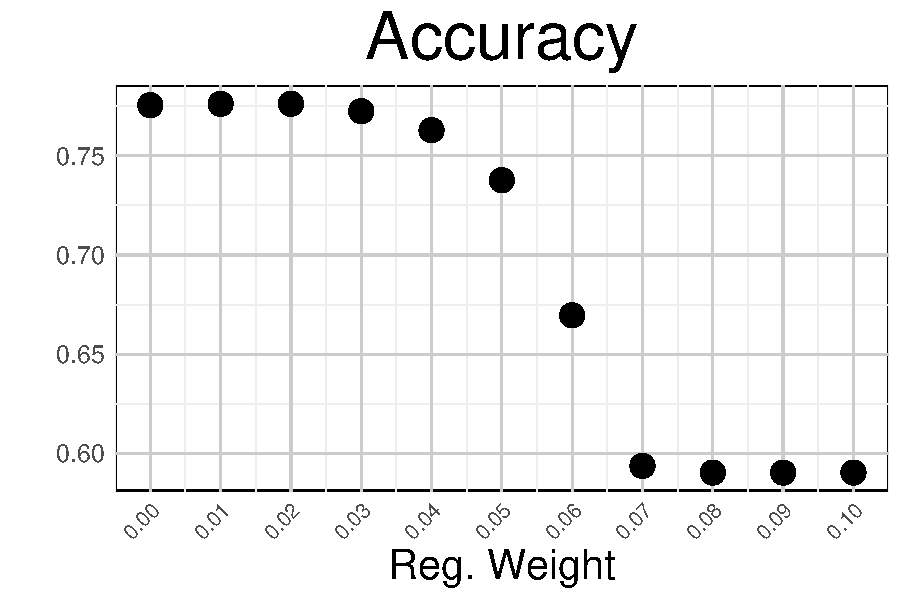
\includegraphics[width=0.24\columnwidth]{figs/regweights/lambdas_Acc.pdf}
%     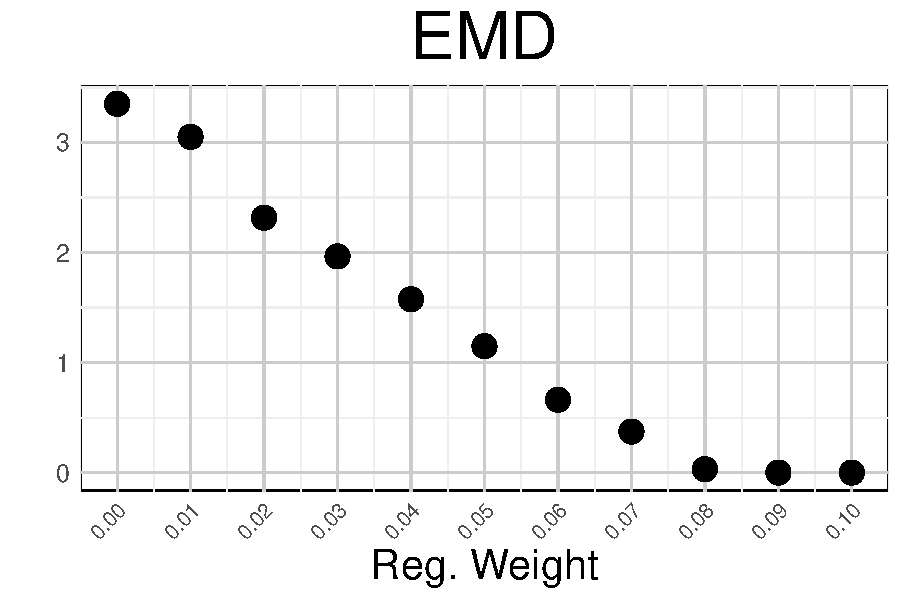
\includegraphics[width=0.24\columnwidth]{figs/regweights/lambdas_DEMD.pdf}
%     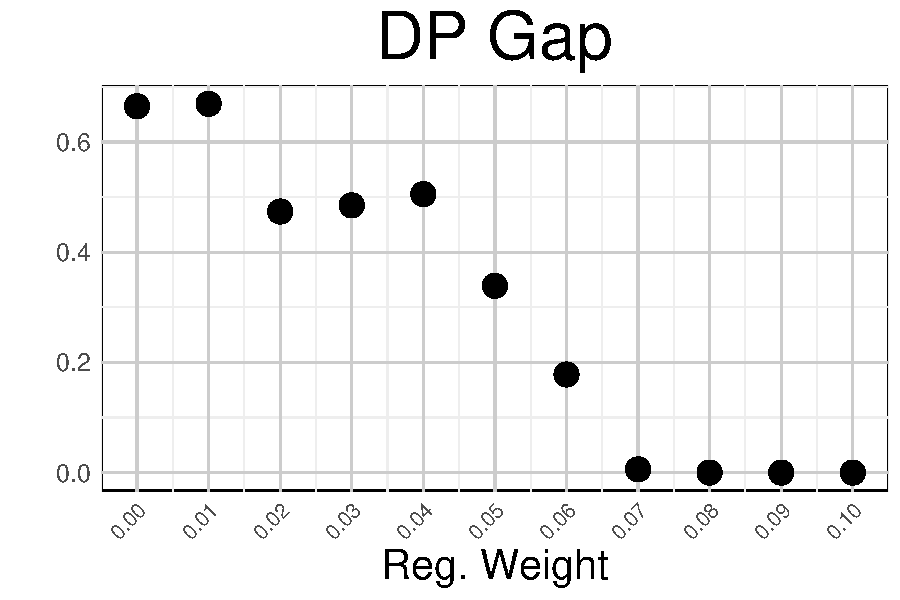
\includegraphics[width=0.24\columnwidth]{figs/regweights/lambdas_DPgap.pdf}
%     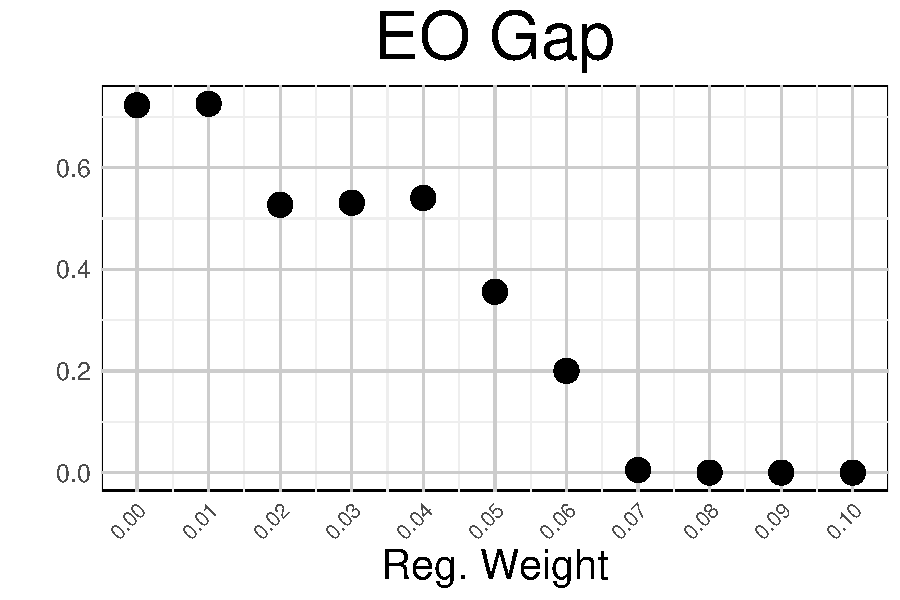
\includegraphics[width=0.24\columnwidth]{figs/regweights/lambdas_EOgap.pdf}
%     \caption{Outcome measures as a function of regularization parameter when our EMD regularizer is used. Output measures of fairness track the upstream EMD constraint, and follow the same accuracy-fairness tradeoff.}
%     \label{fig:reg_sweep}
% \end{figure}

% \begin{table*}[ht]
%     \centering\small
%     \begin{tabular}{llcccccc}
%     \toprule
%         RegType & $\lambda_{reg}$ & Total Acc & MinAcc & MaxAcc & $|DP_{max} - DP_{min}|$ & $|EO_{max} - EO_{min}|$ & D-EMD \\
%         \midrule
%         Log. Reg. & 0.0   & 0.786 & 0.699 & 0.867 & 0.474 & 0.522 & 3.331 \\
%                   & 0.001 & 0.786 & 0.708 & 0.878 & 0.481 & 0.526 & 3.332 \\
%                   & 0.01  & 0.590 & 0.200 & 0.878 & 0.000 & 0.000 & 0.044 \vspace{0.1in}\\
                  
%         2NN       & 0.0   & 0.795 & 0.600 & 0.856 & 0.371 & 0.327 & 3.265 \\
%                   & 0.001 & 0.794 & 0.600 & 0.878 & 0.354 & 0.335 & 2.976 \\
%                   & 0.01  & 0.648 & 0.200 & 0.878 & 0.108 & 0.100 & 0.062 \\
% \bottomrule\\
%     \end{tabular}
%     \caption{Validation results for various models and regularization weights on the ACS Income prediction task including demographic parity
% (DP) and equality of opportunity (EO) spreads. }
%     \label{tab:acsinc}
% \end{table*}


% \begin{table*}[ht]
%     \centering\small
%     \begin{tabular}{llcccccc}
%     \toprule
%         Model & $\lambda_{reg}$ & Total Acc & MinAcc & MaxAcc & $|DP_{max} - DP_{min}|$ & $|EO_{max} - EO_{min}|$ & D-EMD \\
%         \midrule
%         Log. Reg. & 0.0   & 0.786 & 0.699 & 0.867 & 0.474 & 0.522 & 3.331 \\
%                   & 0.001 & 0.786 & 0.708 & 0.878 & 0.481 & 0.526 & 3.332 \\
%                   & 0.01  & 0.590 & 0.200 & 0.878 & 0.000 & 0.000 & 0.044 \vspace{0.1in}\\
                  
%         2NN       & 0.0   & 0.795 & 0.600 & 0.856 & 0.371 & 0.327 & 3.265 \\
%                   & 0.001 & 0.794 & 0.600 & 0.878 & 0.354 & 0.335 & 2.976 \\
%                   & 0.01  & 0.648 & 0.200 & 0.878 & 0.108 & 0.100 & 0.062 \\
% \bottomrule\\
%     \end{tabular}
%     \caption{Validation results for various models and regularization weights on the ACS Income prediction task including demographic parity
% (DP) and equality of opportunity (EO) spreads. }
%     \label{tab:acsinc}
% \end{table*}

% \begin{table*}[ht]
%     \centering\small
%     \begin{tabular}{llcccccc}
%     \toprule
%         Model & $\lambda_{reg}$ & Total Acc & MinAcc & MaxAcc & $|DP_{max} - DP_{min}|$ & $|EO_{max} - EO_{min}|$ & D-EMD \\
%         \midrule
%         Log. Reg.  & 0.0  & 0.769 & 0.500 & 0.824 & 0.194 & 0.194 & 2.200  \\
%                   & 0.01 & 0.769 & 0.500 & 0.824 & 0.194 & 0.185 & 2.124  \\
%                   & 0.1  & 0.546 & 0.500 & 0.632 & 0.000 & 0.000 & 0.093  \vspace{0.1in}\\
%         2NN        & 0.0 & 0.806 & 0.744 & 1.000 & 0.167 & 0.176 & 2.844  \\
%                   & 0.01 & 0.806 & 0.774 & 1.000 & 0.165 & 0.180 & 2.644  \\
%                   & 0.1 & 0.645 & 0.500 & 0.708 & 0.244 & 0.203 & 0.059  \\
% \bottomrule\\
%     \end{tabular}
%     \caption{Validation results for various models and regularization weights on the ACS Employment prediction task including demographic parity
% (DP) and equality of opportunity (EO) spreads.}
%     \label{tab:acsemp}
% \end{table*}
\vspace{-10pt}
\section{Discussion}
\vspace{-10pt}
We presented an efficient solution for solving common practical multi-marginal optimal transport problems.
Our construction is significantly cheaper to compute compared to similar methods,
and allows for large numbers of distributions to be matched in common DNN pipelines. 
Our implementation allows imposing fairness constraints for a variety of applications, including those with many groups, without the need for pairwise measures.
As such, subgroup fairness \citep{kearns2018preventing} is an interesting problem setting that we believe can benefit.
% generalized Earth Mover's objective in the context of a setting where we are interested in bringing a set of distributions closer together. 
% Our construction provides significant computational gains over barycentric approaches for estimating higher dimensional distances. Taking advantage of a direct linear programming formulation, we identify readily available gradients that allow for simple incorporation of the generalized EM measure in existing optimization pipelines. We present empirical evidence that our formulation is faster and valuable in some applications.
%Future work may include exploring the practical application and value of the key theoretical result from \cite{kline2019properties} regarding 
Other properties such as 
Minkowski additivity that have not been 
explicitly leveraged in our experiments may also be a worthwhile direction to explore.
\begin{figure}
    \centering
    % 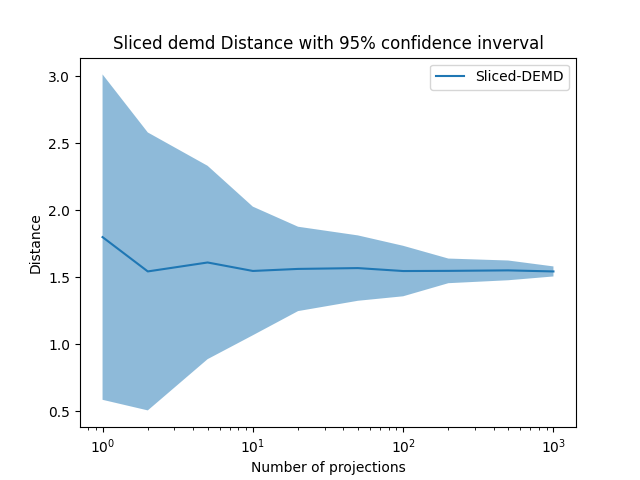
\includegraphics[width=0.32\textwidth]{figs/sliced/demd_mulidim_proj_convergence.png}
    % 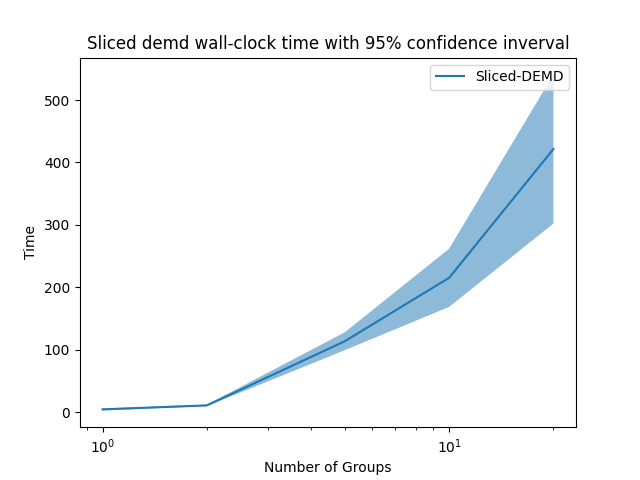
\includegraphics[width=0.32\textwidth]{figs/sliced/groups_vs_distance.png}
    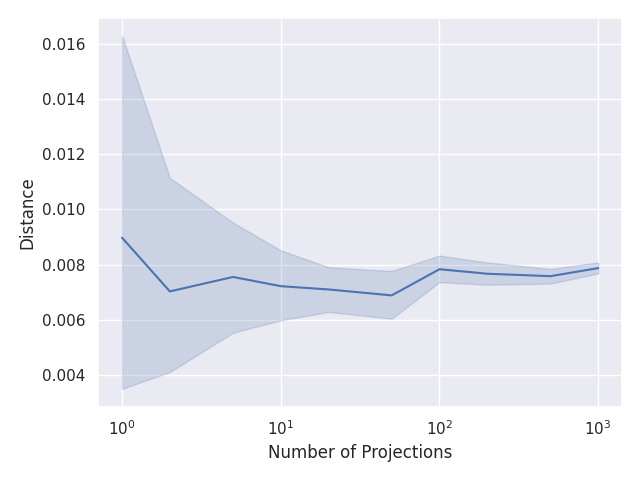
\includegraphics[width=0.4\textwidth]{6_demd/figs/sliced/demd_multidim_proj_convergence_CelebA.png}
    \caption{Sliced DEMD Distance as a function of number of projections.}
    \label{fig:sliced}
\end{figure}
%based on specific use cases.

One limitation of DEMD
is its inability to be directly applied to distributions over multi-dimensional discrete spaces, such as latent spaces common in generative models. 
% The nature of the cost and algorithm suggest this might be a nontrivial, but potentially interesting problem to study.
% In evaluating what might enable these extensions (over images, higher-order tensors, etc.), one important piece is generalizing the Monge cost in some reasonable form, given by an ordering over the multi-dimensional space. Importantly, \textit{a Euclidean embedding of our discrete space does not result in a Monge cost. \ronak{this is true for euc dist, but squared euc dist does satisfy monge}} A sufficient ordering could be defined by a space-filling curve in continuous settings (Hilbert/Peano curves may suffice), but this would not handle arbitrary dimensional spaces unless reduced to the 1-D setting as described above (and adds incremental utility for much more complexity). 
Slicing is a heuristic that has been shown to work well. To evaluate feasibility, we embed distributions over multi-dimensional continuous spaces, take random projections over 1-D spaces, and recompute our DEMD measure. Our gains in the many-distribution setting extend here as well: over a 64-dimensional latent space embedding of CelebA, we can efficiently compute our DEMD measure over all 40 attribute subgroups, and observe convergent behavior w.r.t. the number of projections.% (Fig.~\ref{fig:sliced}).
%Our scaling above enables distance computations in this setting as well, See Appendix~\ref{sec:app-multi} for additional details.

%{\bf Ethical Considerations.} Machine learning (ML) models that have skewed performance on subsets of individuals are increasingly of concern within the community. Our proposed DEMD can be used to address general fairness problems in ML, particularly where group disparities are to be mitigated. 
%We aim to add another tool in the fairness toolbox available to ML practitioners, alongside important cultural procedures promoting equitable use, from data sources to model outputs and human audits.

% While the goal of our tool is to mitigate group disparities in practice, it is not a catch-all solution to fairness problems in machine learning. Although the results presented are promising, any application of DEMD in practice should, as always, be done with care, including both algorithmic procedures such as full hyperparameter optimization and cross validation, as well as independent, human audits of all models and results.

% An intriguing direction for future work could exploit an unexplored feature of the generalized EM functional. In~\cite{kline2019properties}, it is shown that the optimal objective value of the generalized EM program is {\em Minkowski additive} in the program data. This is a highly unusual property. It may be possible to exploit this property to other use cases in machine learning models, as well as other theoretical investigations.


% \textbf{Minkowski Additivity}
% Means we can also separate and combine functionals on different sets, and optimizing one set until it is a subset of another allows us to take advantage of the additivity.

% \textbf{Fairness Intrinsic Dimensionality}
% The support outlined above is a measure of fairness dimensionality.
% A completely fair algorithm would have a dimensionality of 0.

